\subsection{Obtaining conformal confidence sets with increasing combination functions}\label{A:CF}
As discussed in Remark \ref{rmk:max} the results of Sections \ref{SS:MCS} and \ref{SS:joint} can be generalized to a wider class of combination functions. 
\begin{definition}
	We define a suitable combination function to be a function $C: \mathcal{P}(\mathcal{V}) \times \mathcal{X} \rightarrow \mathbb{R}$  which is increasing in the sense that for all sets $\mathcal{A} \subseteq \mathcal{V}$ and each $v \in \mathcal{A} $, $C(v, X) \leq C(\mathcal{A}, X)$ for all $X \in \mathcal{X}$. 
\end{definition}
The maximum is a suitable combination function since $X(v) = \max_{v \in \lbrace v \rbrace } X(v) \leq \max_{v \in \mathcal{A}} X(v)$. As such this framework directly generalizes the results of the main text. 
%Moreover for each $1\leq i \leq n + 1$, let $$\tau'_i = C(\lbrace v \in \mathcal{V}: Y_i(v) = 0\rbrace, f_O(s(X_i))) $$and $$\gamma'_i= C(\lbrace v \in \mathcal{V}: Y_i(v) = 1\rbrace, f_I(-s(X_i))).$$

We can construct generalized marginal confidence sets as follows.
\begin{theorem}\label{thm:innergen}
	(Marginal inner set)
	Under Assumptions \ref{ass:ex} and \ref{ass:indep}, given $\alpha_1 \in (0,1)$, define 
	\begin{equation*}
		\lambda_I(\alpha_1) = \inf\left\lbrace \lambda: \frac{1}{n} \sum_{i = 1}^n 1\left[ C(\lbrace v \in \mathcal{V}: Y_i(v) = 1\rbrace, f_I(s(X_i))) \leq \lambda \right] \geq \frac{\lceil (1-\alpha_1)(n+1) \rceil}{n} \right\rbrace,
	\end{equation*}
 	for a suitable combination function $C$, and define $I(X) = \lbrace v \in \mathcal{V}: C(v, f_I(s(X))) >\lambda_I(\alpha_1)  \rbrace $. Then,
	\begin{equation}\label{eq:probstat}
		\mathbb{P}\left( I(X_{n+1}) \subseteq\lbrace v\in \mathcal{V}: Y_{n+1}(v) = 1 \rbrace \right) \geq 1 - \alpha_1.
	\end{equation}
\end{theorem}
The proof follows that of Theorem \ref{thm:inner}. The key observation is that for any suitable combination function $C$,  given $\lambda \in \mathbb{R}$, $\mathcal{A} \subseteq \mathcal{V} $ and $X \in \mathcal{X}$, $C(\mathcal{A}, X) \leq \lambda$ implies that $C(v, X) \leq \lambda$. This is the relevant property of the maximum which we used for the results in the main text. For the outer set we similarly have the following.
\begin{theorem}\label{thm:genouter}
	(Marginal outer set)
	Under Assumptions \ref{ass:ex} and \ref{ass:indep}, given $\alpha_2 \in (0,1)$, define 
	\begin{equation*}
		\lambda_O({\alpha_2})= \inf\left\lbrace \lambda: \frac{1}{n} \sum_{i = 1}^n 1\left[ C(\lbrace v \in \mathcal{V}: Y_i(v) = 0\rbrace, -f_O(s(X_i))) \leq \lambda \right] \geq \frac{\lceil (1-\alpha_2)(n+1) \rceil}{n} \right\rbrace.
	\end{equation*}
	for a suitable combination function $C$, and let $O(X) = \lbrace v \in \mathcal{V}: C(v, -f_O(s(X))) \leq \lambda_O(\alpha_2)  \rbrace $. Then,
	\begin{equation}\label{eq:probstat}
		\mathbb{P}\left( \lbrace v\in \mathcal{V}: Y_{n+1}(v) = 1 \rbrace \subseteq O(X_{n+1}) \right) \geq 1 - \alpha_2.
	\end{equation}
\end{theorem}
Joint results can be analogously obtained. 

\subsection{Obtaining confidence sets from risk control}\label{risk2con}
We can alternatively establish Theorems \ref{thm:inner} and \ref{thm:innergen} using an argument from risk control \citep{Angelopoulos2022}. In particular, given an image pair $(X,Y)$ and $\lambda \in \mathbb{R}$, let $$I_\lambda(X) =  \lbrace v \in \mathcal{V}: f_I(s(X), v) > \lambda \rbrace.$$ Define a loss function, $L:\mathcal{P}(\mathcal{V}) \times \mathcal{Y} \rightarrow \mathbb{R}$ which sends $(X,Y)$ to 
\begin{equation*}
	L(I_\lambda(X), Y) = 1\left[ I_\lambda(X) \not \subseteq\lbrace v\in \mathcal{V}: Y(v) = 1 \rbrace \right].
\end{equation*}
For $i = 1, \dots, n + 1$, let 	$L_i(\lambda) = 	L(I_\lambda(X_i), Y_i)$. Arguing as in the proof of Theorem \ref{thm:inner} it follows that $L_i(\lambda) = 1[\tau_i > \lambda]$. Then applying Theorem 1 of \cite{Angelopoulos2022} it follows that 
\begin{equation*}
	\mathbb{E}\left[ L_{n+1}(\hat{\lambda})\right] \leq \alpha_1,
\end{equation*}
where $\hat{\lambda} = \inf\left\lbrace \lambda: \frac{1}{n}\sum_{i = 1}^n L_i(\lambda) \leq \alpha_1 - \frac{1-\alpha_1}{n}\right\rbrace$. Arguing as in Appendix A of \citep{Angelopoulos2022} it follows that 
	\begin{equation*}
	\hat{\lambda} = \inf\left\lbrace \lambda: \frac{1}{n} \sum_{i = 1}^n 1\left[ \tau_i\leq \lambda \right] \geq \frac{\lceil (1-\alpha_1)(n+1) \rceil}{n}\right\rbrace = \lambda_I(\alpha_1),
\end{equation*}
and so $I(X) = I_{\hat{\lambda}}(X)$. As such 	
\begin{equation}\label{eq:probstat2}
	\mathbb{P}\left( I(X_{n+1}) \subseteq\lbrace v\in \mathcal{V}: Y_{n+1}(v) = 1 \rbrace \right) = 1 - \mathbb{E}\left[ L_{n+1}(\hat{\lambda})\right]  \geq 1 - \alpha_1, 
\end{equation}
and we recover the desired result. Arguing similarly it is possible to establish a proof of Theorem \ref{thm:outer}.

\subsection{Deriving confidence sets from bounding boxes}\label{AA:BBtheory}
We can use our results in order to provide valid inference for bounding boxes via an adaption of the approach of \cite{Andeol2023}. In particular given $Z \in \mathcal{Y}$, let $B_{I, \max}(Z)$ be the largest box which can be contained within the set $\lbrace v\in \mathcal{V}: Z(v) = 1 \rbrace$ and let $ B_{O, \min}(Z)$ be the smallest box which contains the set $\lbrace v\in \mathcal{V}: Z(v) = 1 \rbrace$. Given $Y \in \mathcal{Y}, $ let $cc(Y) \subseteq \mathcal{P}(\mathcal{V})$ denote the set of connected components of the set $\lbrace v\in \mathcal{V}: Y(v) = 1 \rbrace$ for a given connectivity criterion (which we take to be $4$ in our examples), and note that these components can themselves be identifed as elements of $\mathcal{Y}$. Define 
$$B_I(Y) = \cup_{c \in cc(Y)} B_{I, \max}(c) \text{ and } B_O(Y) = \cup_{c \in cc(Y)} B_{O, \min}(c)$$
to be the unions of the largest inner and smallest outer boxes of the connected components of the image $Y$, respectively. Then define
$$\hat{B}_I(s(X)) = \cup_{c \in cc(\hat{M}(X)) } B_{I, \max}(c) \text{ and } \hat{B}_O(s(X)) = \cup_{c \in cc(\hat{M}(X))} B_{O, \min}(c)$$
to be the unions of the largest inner and smallest outer boxes of the connected components of the predicted mask $\hat{M}(X)$, respectively. Note that this is well-defined as $\hat{M}(X)$ is a function of $s(X)$.

For the remainder of this section we shall assume that $\mathcal{V} \subset \mathbb{R}^2$, this is not strictly necessary but will help to simplify notation. Given $u,v \in \mathcal{V}$, write $u = (u_1, u_2)$ and $v = (v_1, v_2)$ and let $\rho(u,v) = \max \left( |u_1 - v_1|, |u_2 - v_2| \right)$ be the chessboard metric. 
\begin{definition}\label{dfn:BBS}
	(Bounding box scores) For each $X \in \mathcal{X}$ and $v \in \mathcal{V}$, let
	\begin{equation*}
		b_I(s(X), v) = d_{\rho}(\hat{B}_I(s(X)), v) \text{ and } b_O(s(X), v) = d_{\rho}(\hat{B}_O(s(X)), v) 
	\end{equation*}
be the distance transformed scores based on the chessboard distance to the predicted inner and outer box collections $\hat{B}_I(s(X))$ and $\hat{B}_O(s(X))$, respectively. We also define a combination of these $b_M$, primarily for the purposes of plotting in Figure \ref{fig:learning}, as follows. Let $b_M(s(X), v) = b_O(s(X),v)$ for each $v \not\in \hat{B}_O(s(X))$ and let $b_M(s(X), v) = \max(b_I(s(X),v), 0) $ for $v \in \hat{B}_O(s(X))$. We shall write $b_I(s(X)) \in \mathcal{X}$ to denote the image which has $b_I(s(X))(v) = 	b_I(s(X), v)$ and similarly for $b_O(s(X))$ and $b_M(s(X))$. 
%An illustration of these scores for two example tumors is shown in Figure XXX.
\end{definition}
Now consider the sequences of image pairs $(X_i, B_i^I)_{i = 1}^n$ and $(X_i, B_i^O)_{i = 1}^n$. These both satisfy exchangeability and so, applying Theorems \ref{thm:innergen} and \ref{thm:genouter}, we obtain the following bounding box validity results.
\begin{corollary}\label{thm:boxinnergen}
	(Marginal inner bounding boxes)
	Suppose Assumption \ref{ass:ex} holds and that $(X_i, Y_i)_{i = 1}^{n+1}$ is independent of the functions $s$ and $b_I$.  Given $\alpha_1 \in (0,1)$, define 
	\begin{equation}
		\lambda_I(\alpha_1) = \inf\left\lbrace \lambda: \frac{1}{n} \sum_{i = 1}^n 1\left[ C(B^I_i, b_I(s(X_i))) \leq \lambda \right] \geq  \frac{\lceil (1-\alpha_1)(n+1) \rceil}{n} \right\rbrace,
	\end{equation}
	for a suitable combination function $C$, and define $I(X) = \lbrace v \in \mathcal{V}: C(v, b_I(s(X))) >\lambda_I(\alpha_1)  \rbrace $. Then,
	\begin{equation*}\label{eq:probstat}
		\mathbb{P}\left( I(X_{n+1}) \subseteq B^I_{n+1} \subseteq\lbrace v\in \mathcal{V}: Y_{n+1}(v) = 1 \rbrace \right) \geq 1 - \alpha_1.
	\end{equation*}
\end{corollary}
\begin{corollary}\label{thm:boxgenouter}
	(Marginal outer bounding boxes)
	Suppose Assumption \ref{ass:ex} holds and that $(X_i, Y_i)_{i = 1}^{n+1}$ is independent of the functions $s$ and $b_O$. Given $\alpha_2 \in (0,1)$, define 
	\begin{equation}
		\lambda_O({\alpha_2})= \inf\left\lbrace \lambda: \frac{1}{n} \sum_{i = 1}^n 1\left[ C(B^O_i, -b_O(s(X_i))) \leq \lambda \right] \geq  \frac{\lceil (1-\alpha_2)(n+1) \rceil}{n} \right\rbrace.
	\end{equation}
	for a suitable combination function $C$, and let $O(X) = \lbrace v \in \mathcal{V}: C(v, -b_O(s(X))) \leq \lambda_O(\alpha_2)  \rbrace $. Then,
	\begin{equation*}\label{eq:probstat}
		\mathbb{P}\left( \lbrace v\in \mathcal{V}: Y_{n+1}(v) = 1 \rbrace \subseteq B^O_{n+1} \subseteq O(X_{n+1}) \right) \geq 1 - \alpha_2.
	\end{equation*}
\end{corollary}
Joint results can be obtained in a similar manner to those in Section \ref{SS:joint}.

\newpage
\subsection{Additional settings for polyps segmentation}
\subsubsection{Additional examples from the learning dataset}

\begin{figure}[h!]
	%	\centering
	\begin{center}
		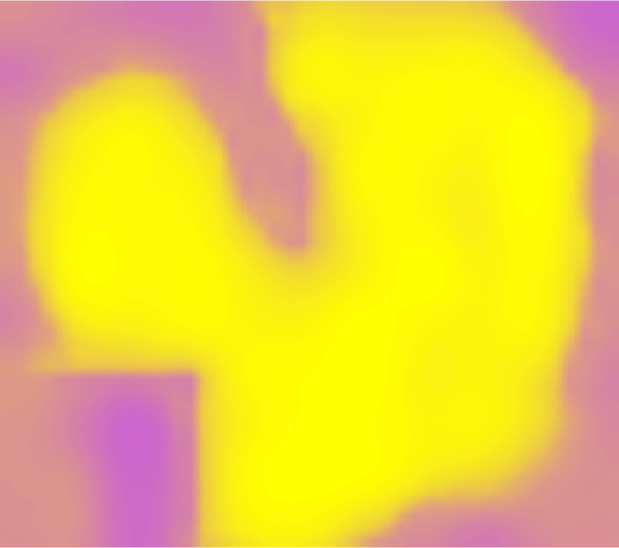
\includegraphics[width=0.24\textwidth]{../figures/learning/scores/772.png}
		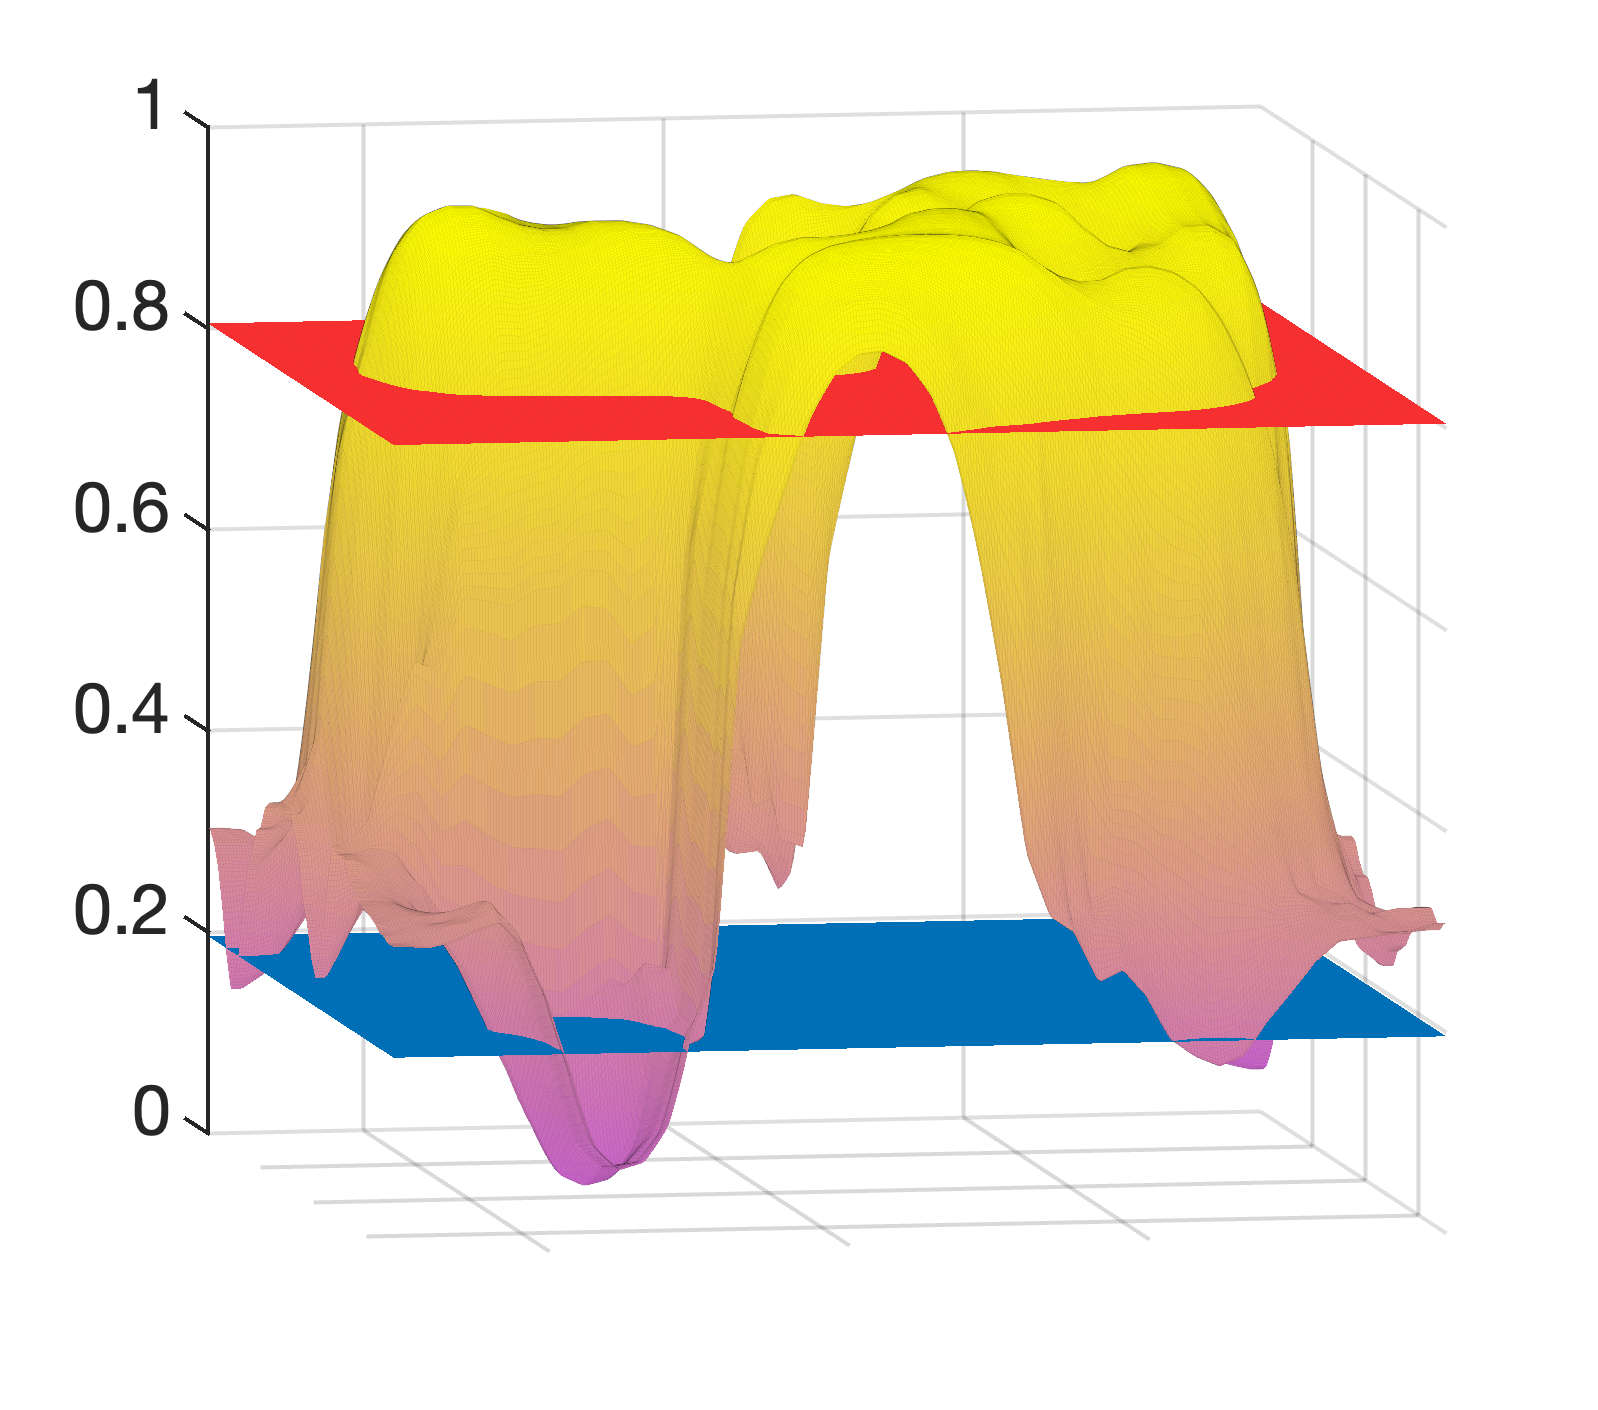
\includegraphics[width=0.24\textwidth]{../figures/learning/score_surf/772.png}	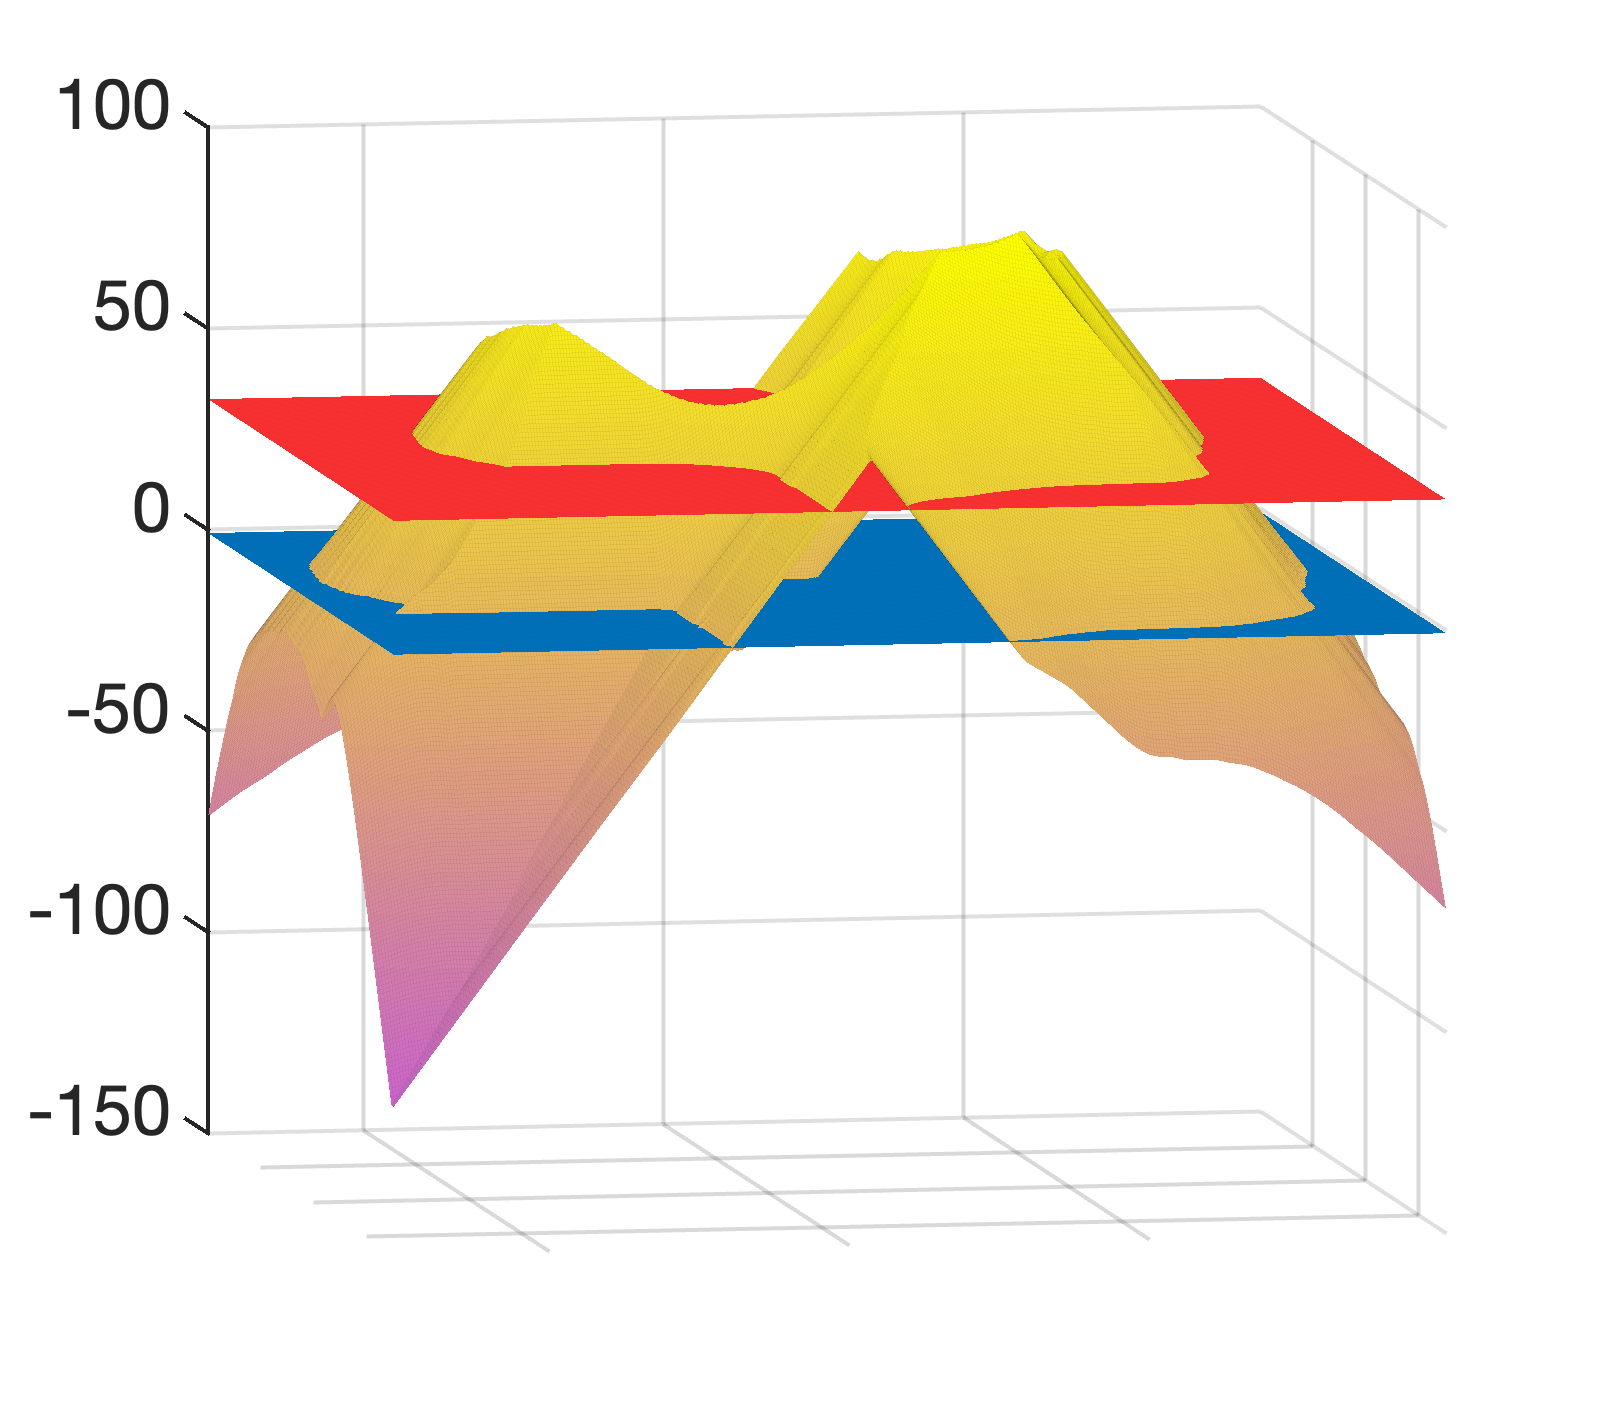
\includegraphics[width=0.24\textwidth]{../figures/learning/dist_surf/772.png}
		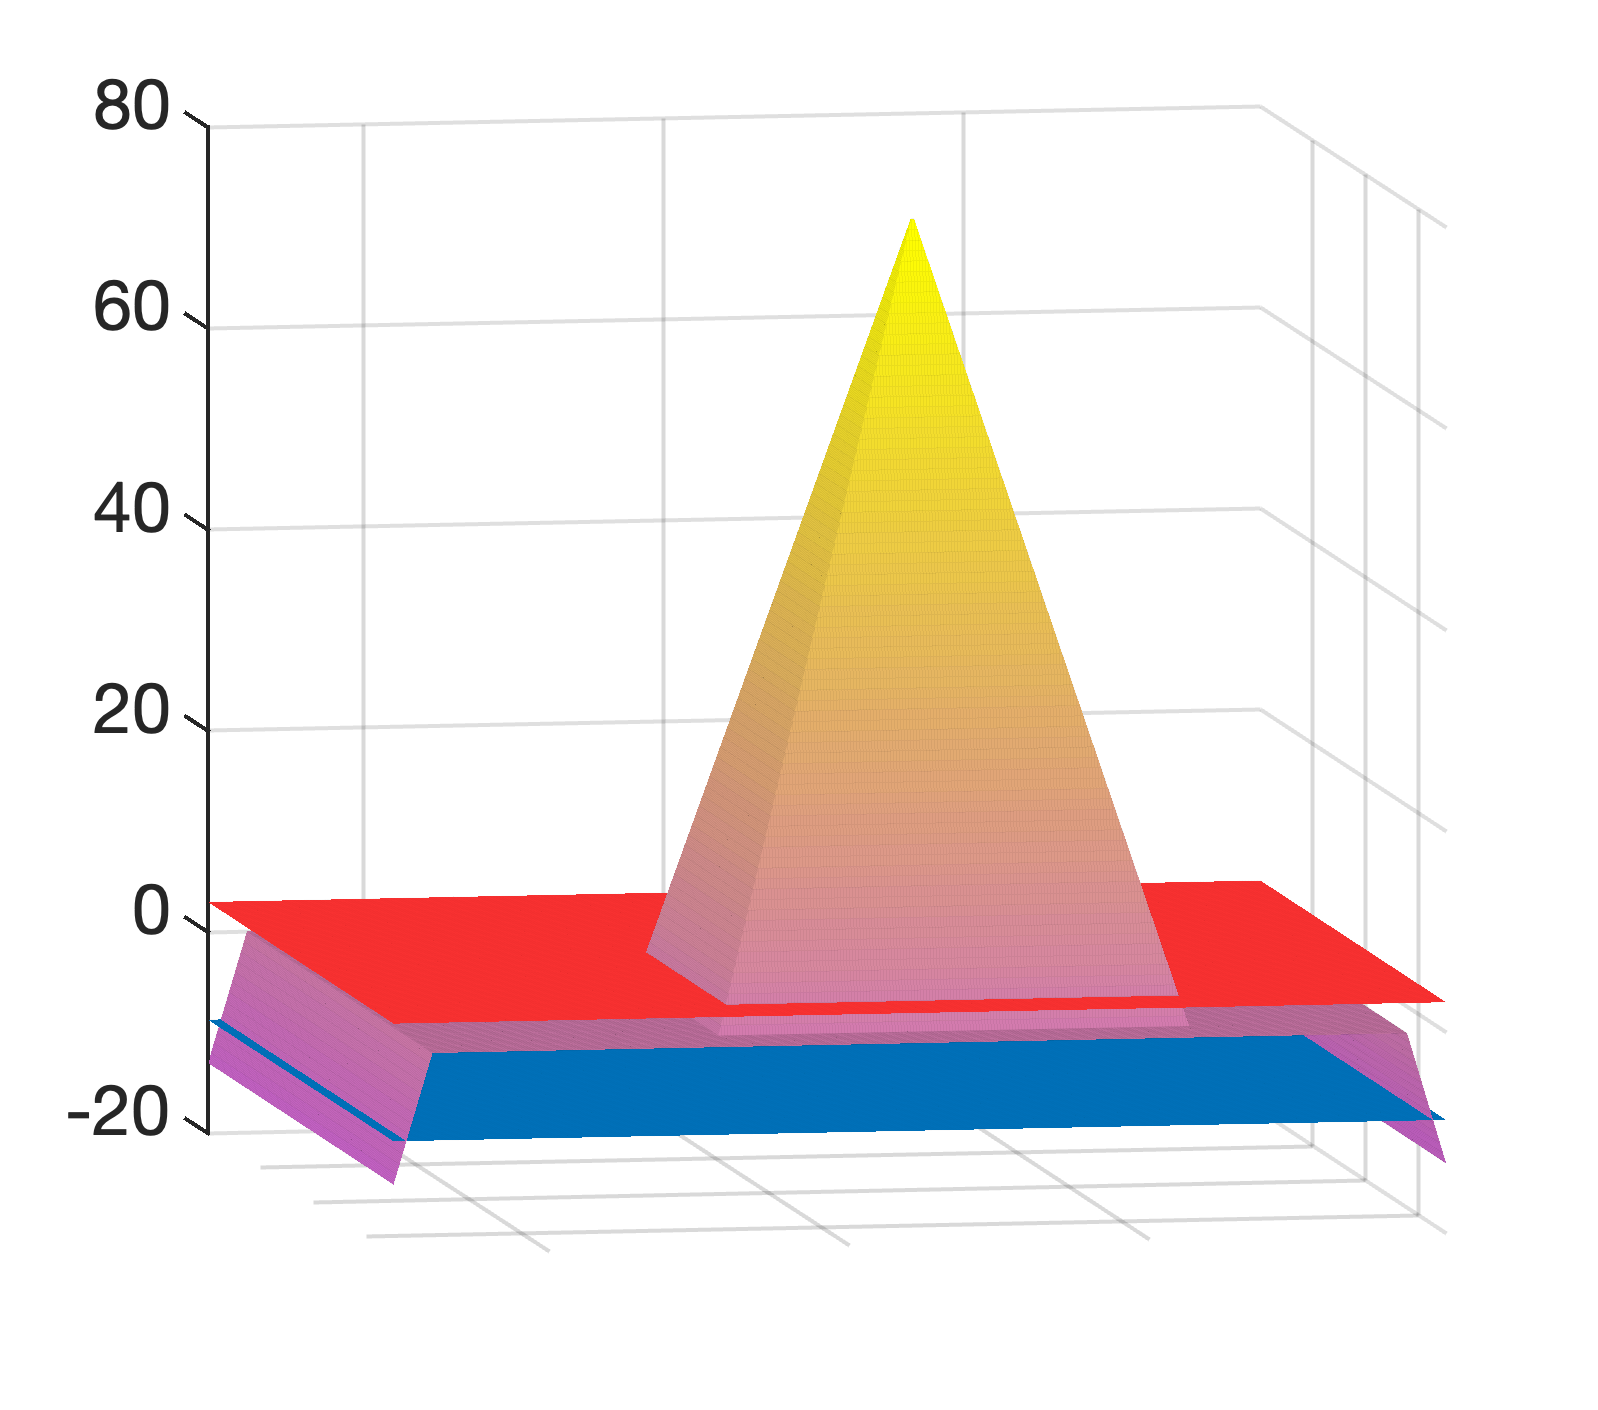
\includegraphics[width=0.24\textwidth]{../figures/learning/dist_bt_surf/772.png}\\
		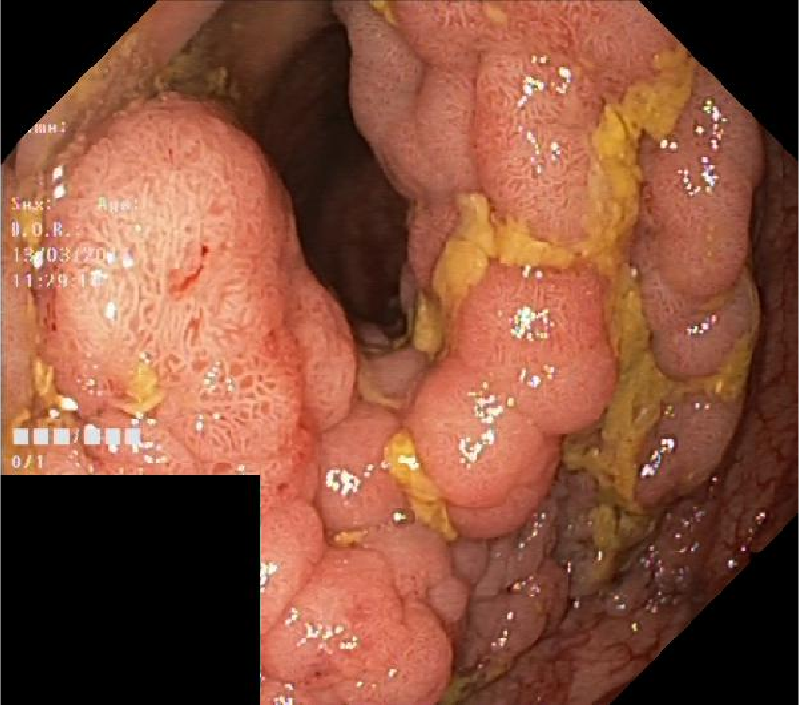
\includegraphics[width=0.24\textwidth]{../figures/learning/images/772.png}
		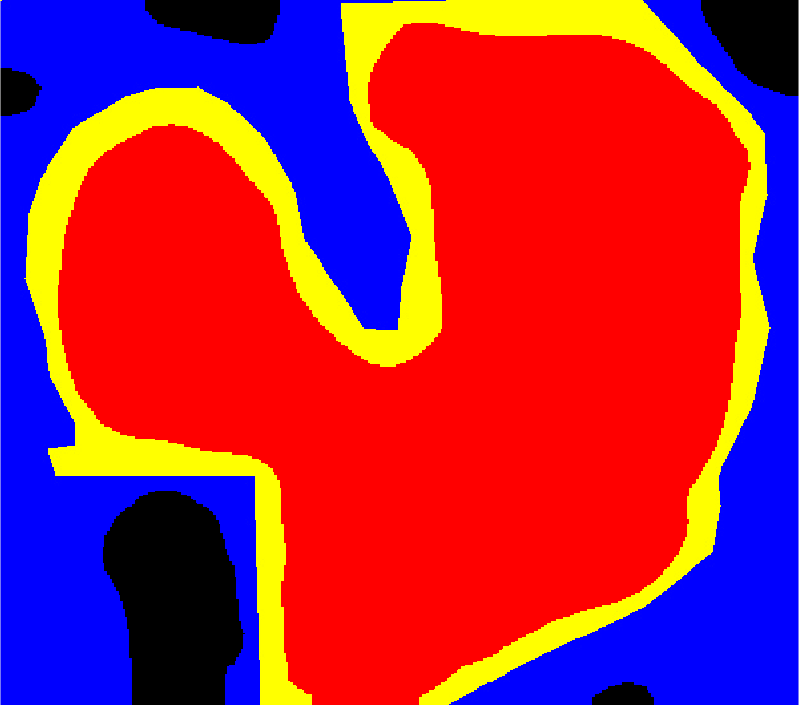
\includegraphics[width=0.24\textwidth]{../figures/learning/score_crs_marginal90/772.png}
		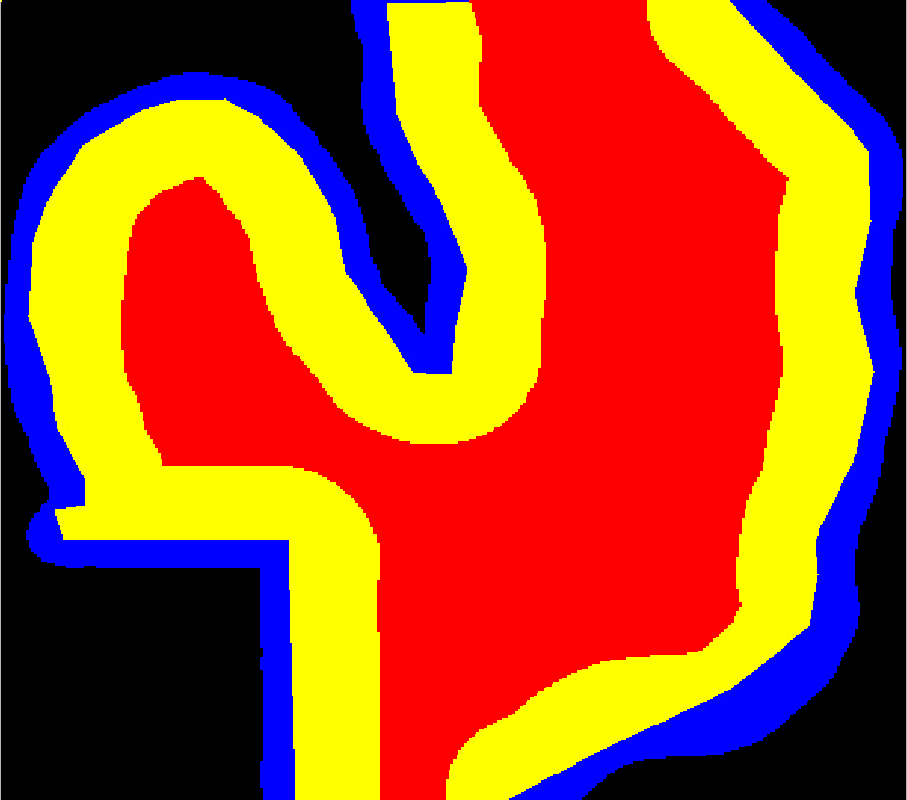
\includegraphics[width=0.24\textwidth]{../figures/learning/dist_crs_marginal90/772.png}
		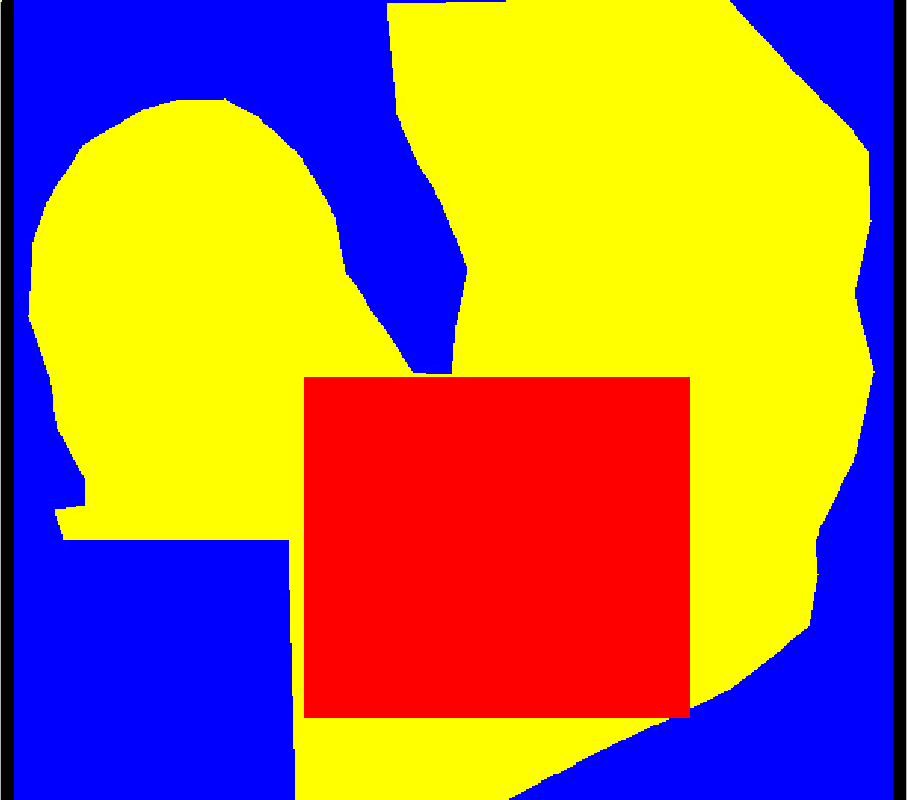
\includegraphics[width=0.24\textwidth]{../figures/learning/dist_bt_crs_marginal90/772.png}\\
		\vspace{0.5cm}
		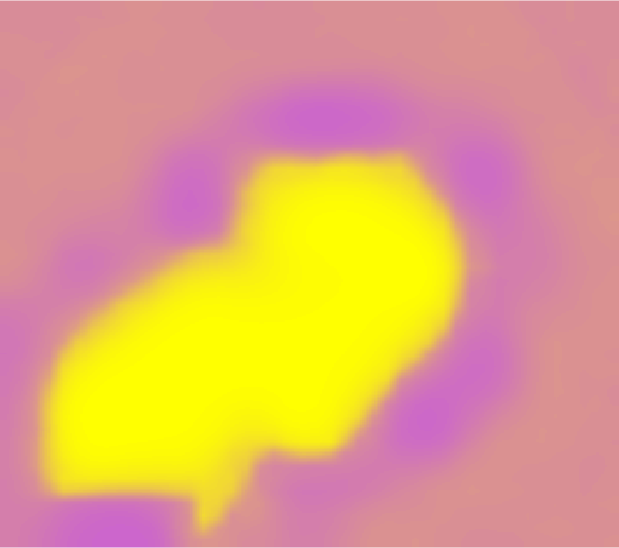
\includegraphics[width=0.24\textwidth]{../figures/learning/scores/202.png}
		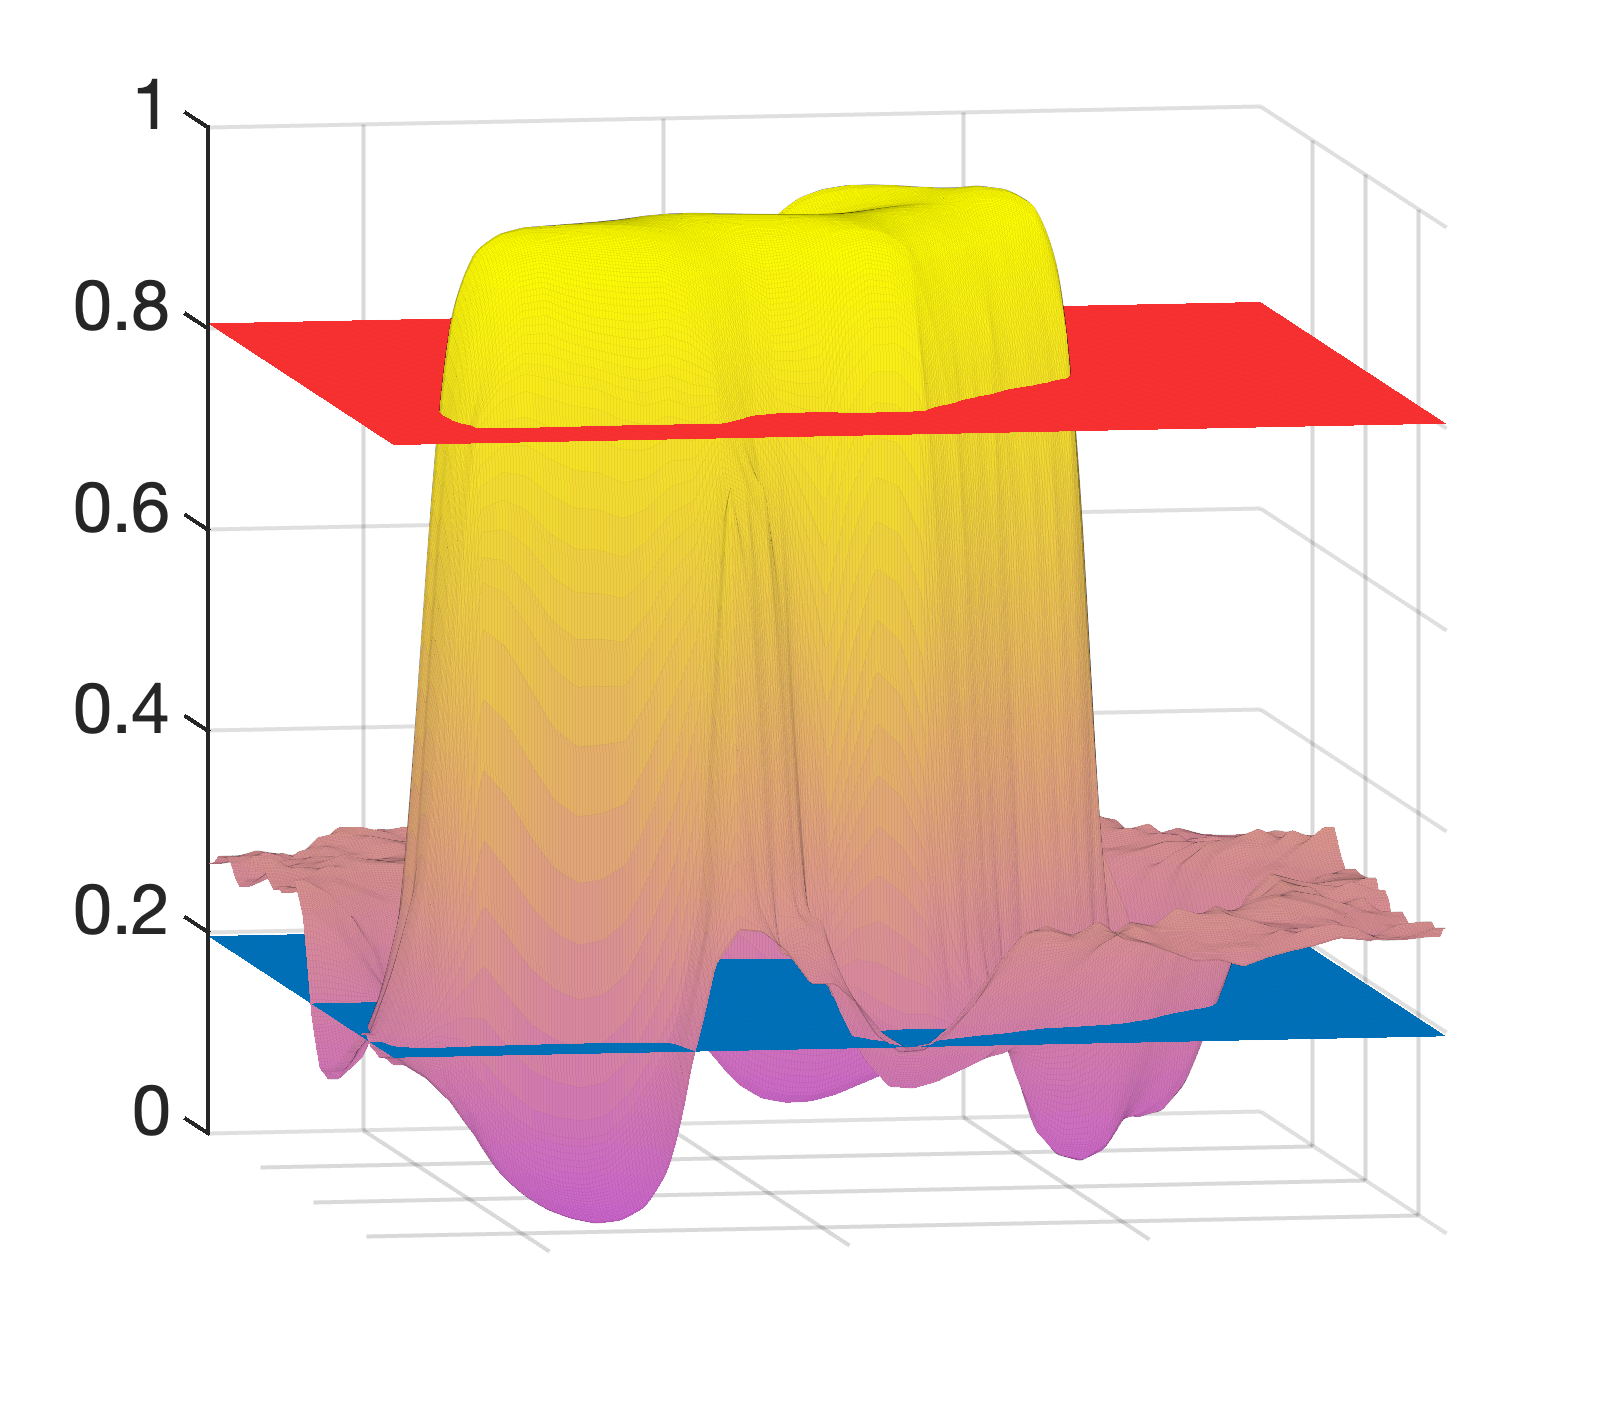
\includegraphics[width=0.24\textwidth]{../figures/learning/score_surf/202.png}	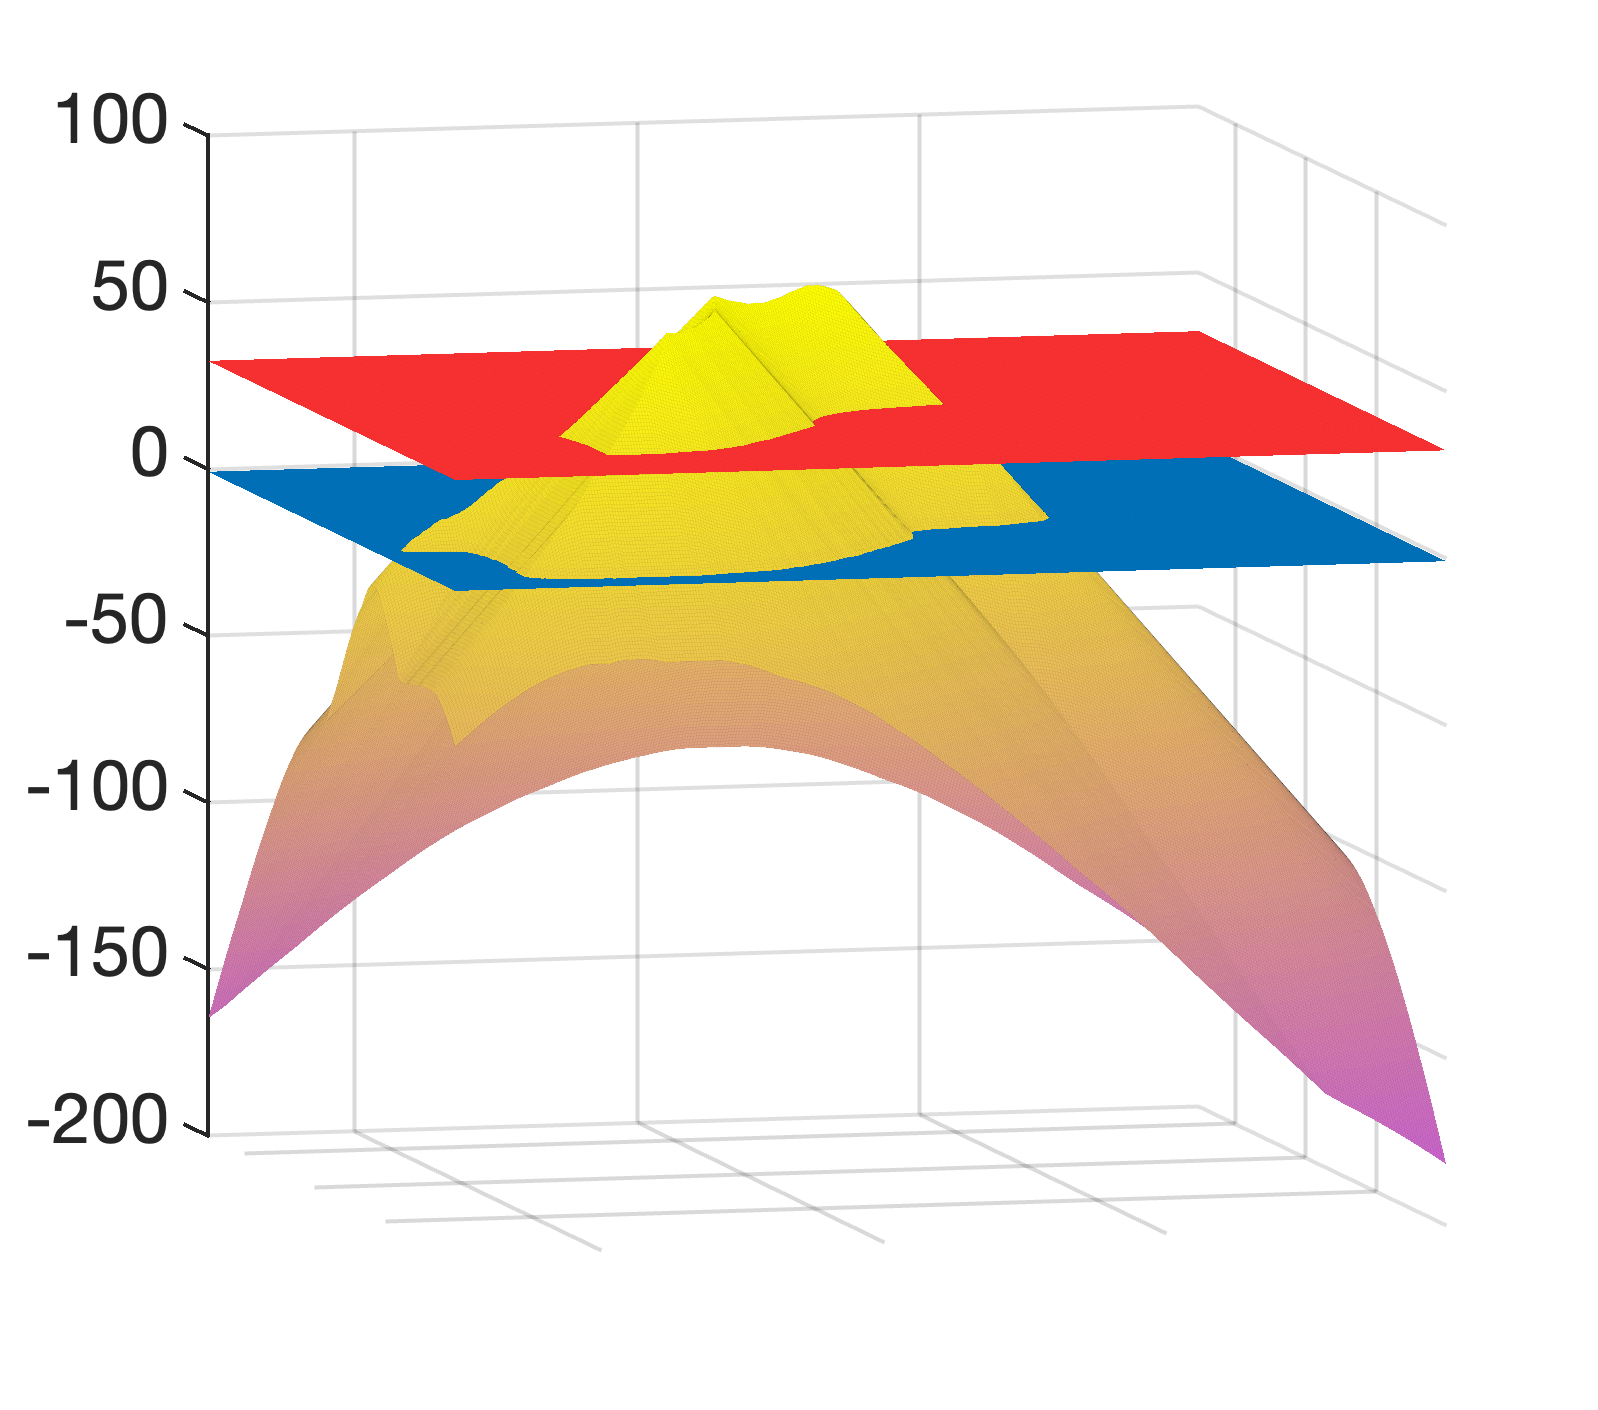
\includegraphics[width=0.24\textwidth]{../figures/learning/dist_surf/202.png}
		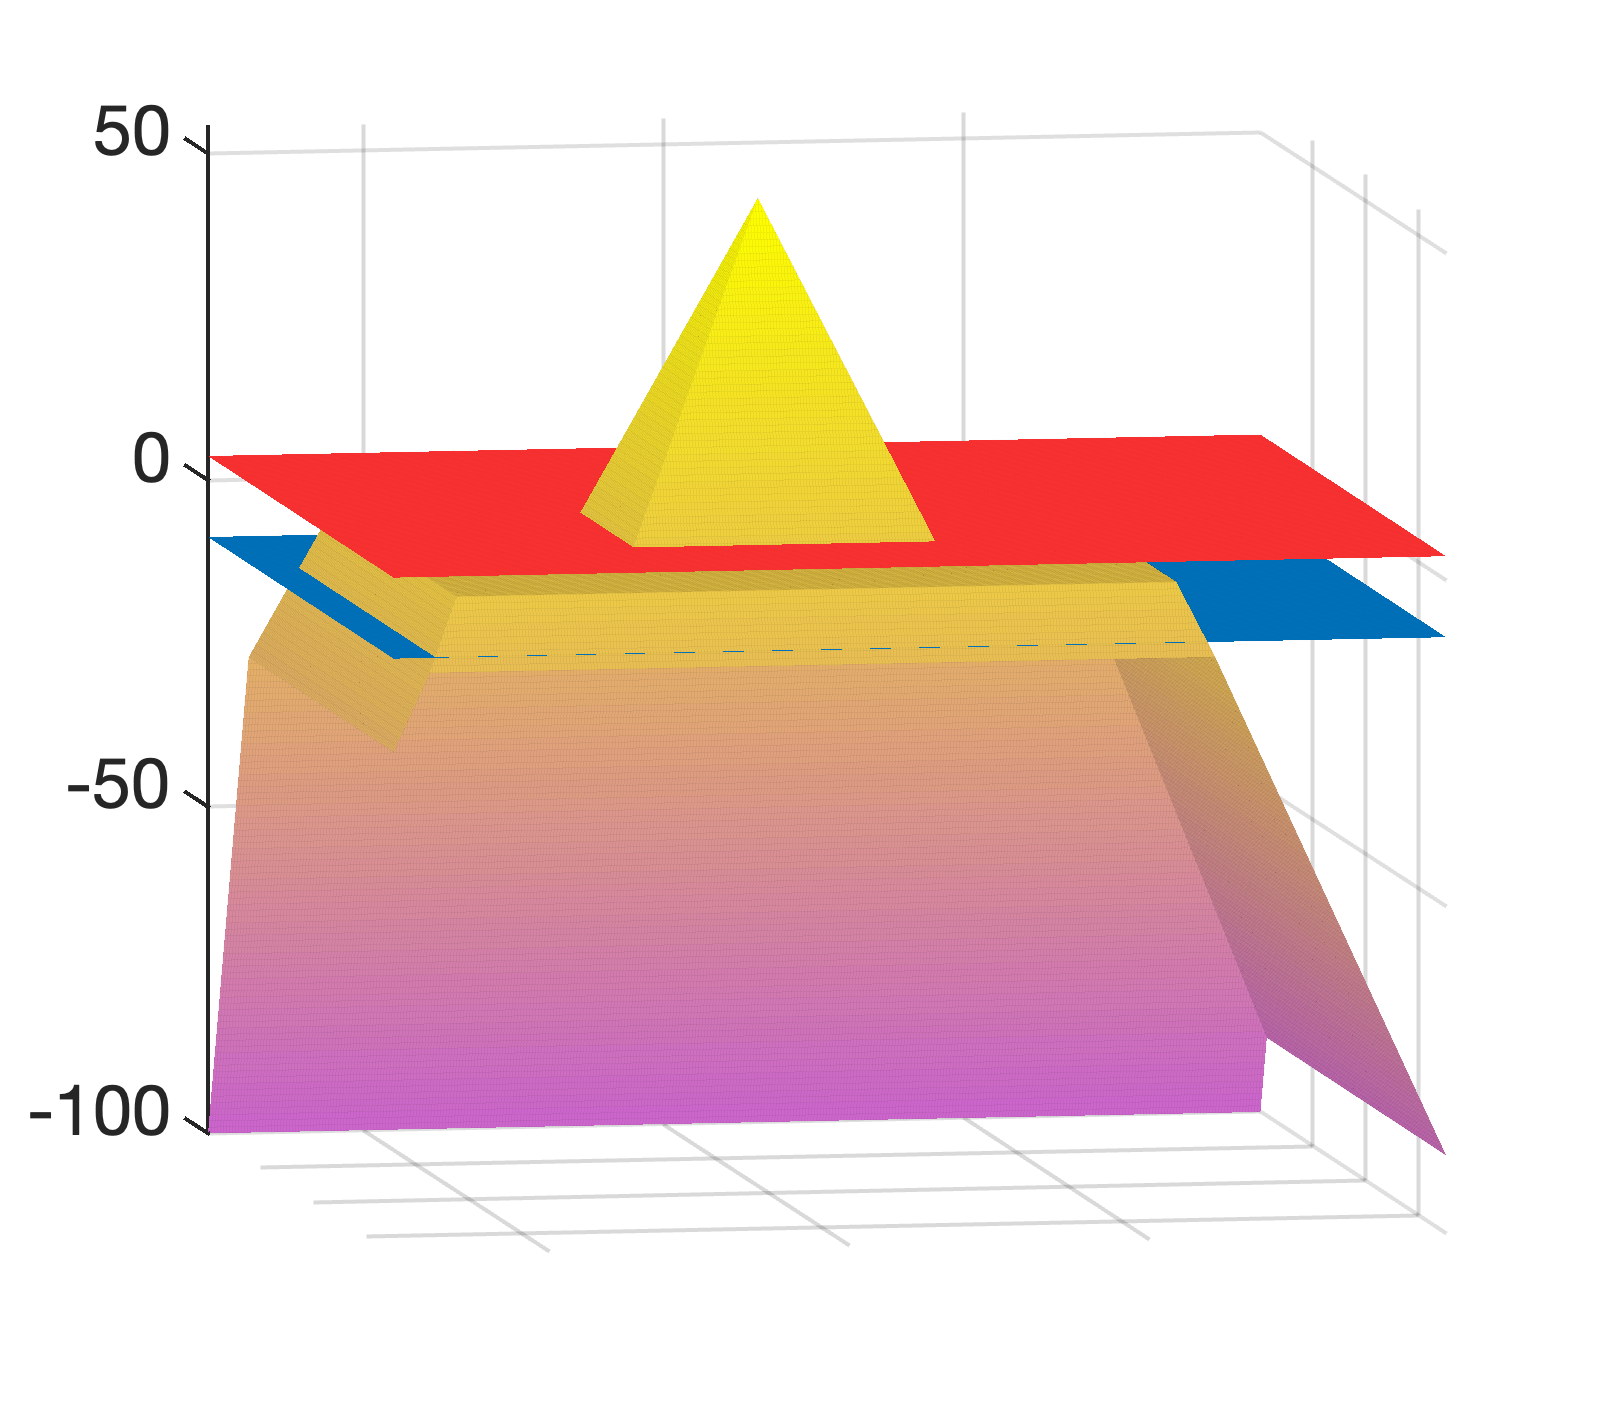
\includegraphics[width=0.24\textwidth]{../figures/learning/dist_bt_surf/202.png}\\
		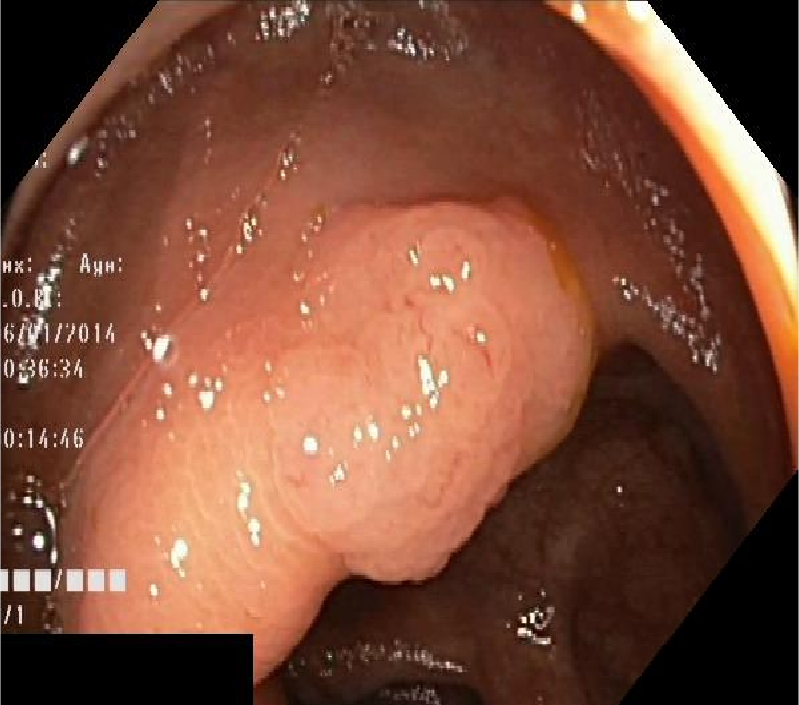
\includegraphics[width=0.24\textwidth]{../figures/learning/images/202.png}
		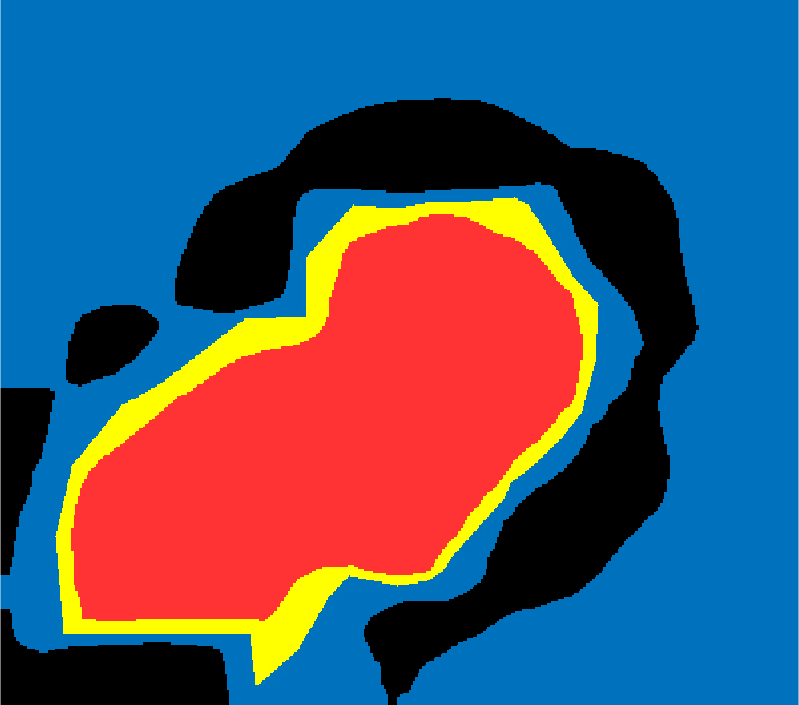
\includegraphics[width=0.24\textwidth]{../figures/learning/score_crs_marginal90/202.png}
		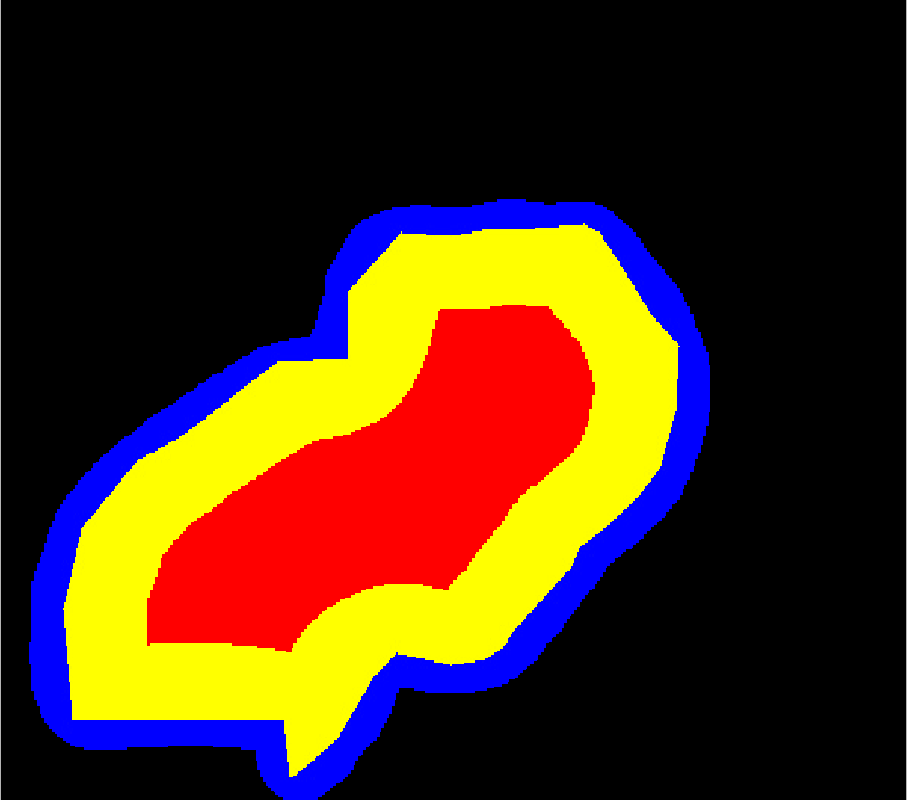
\includegraphics[width=0.24\textwidth]{../figures/learning/dist_crs_marginal90/202.png}
		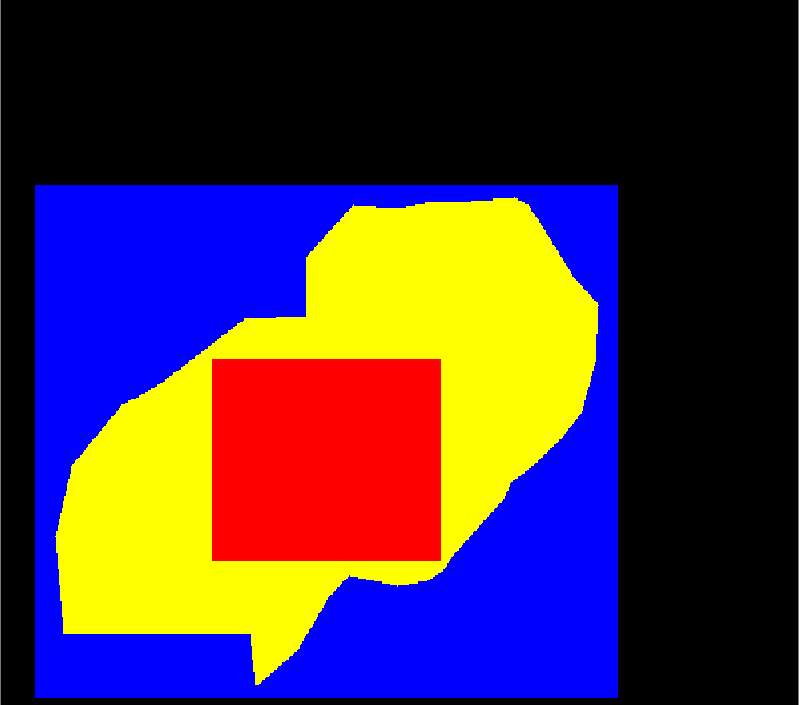
\includegraphics[width=0.24\textwidth]{../figures/learning/dist_bt_crs_marginal90/202.png}\\
			\vspace{0.5cm}
		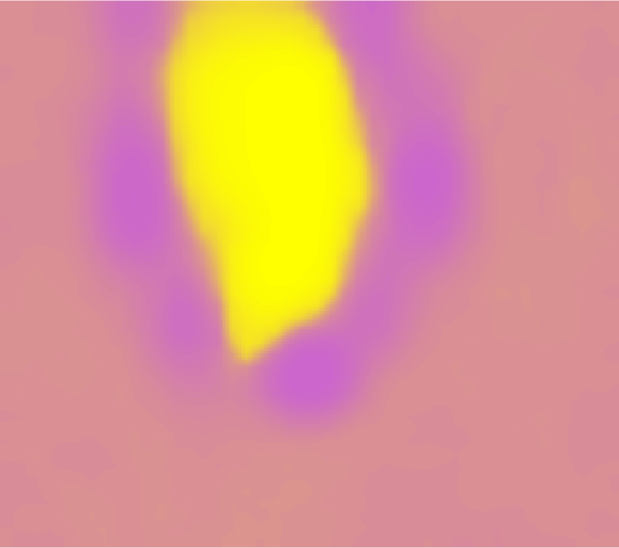
\includegraphics[width=0.24\textwidth]{../figures/learning/scores/54.png}
		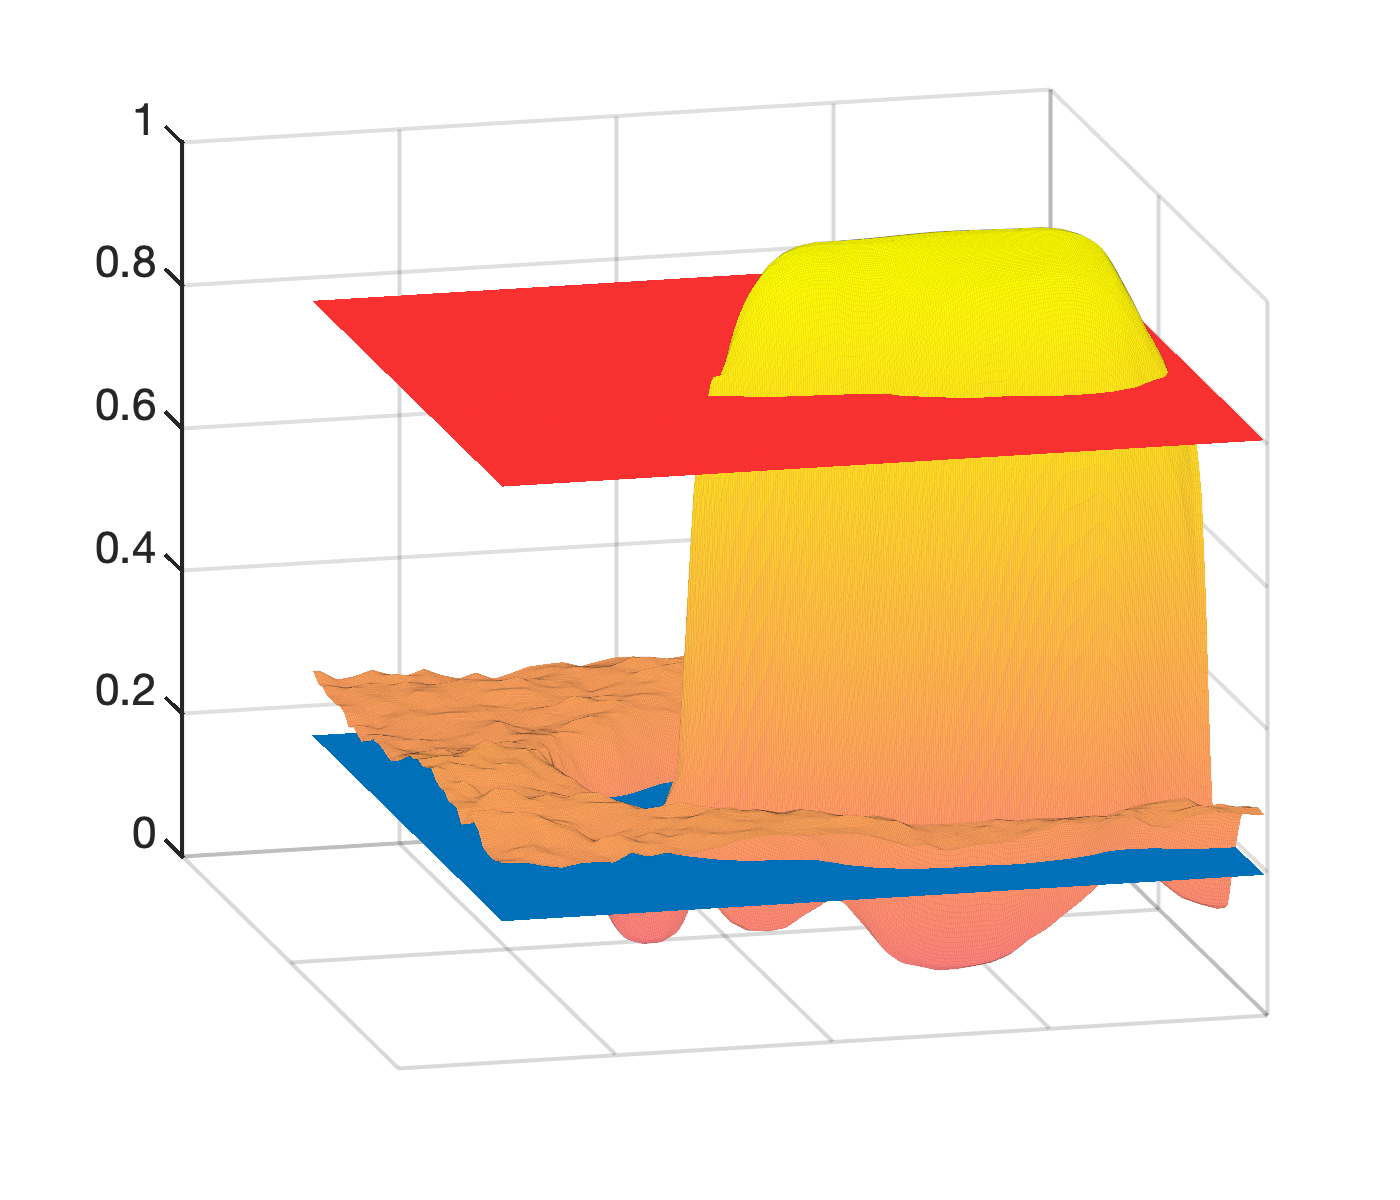
\includegraphics[width=0.24\textwidth]{../figures/learning/score_surf/54.png}	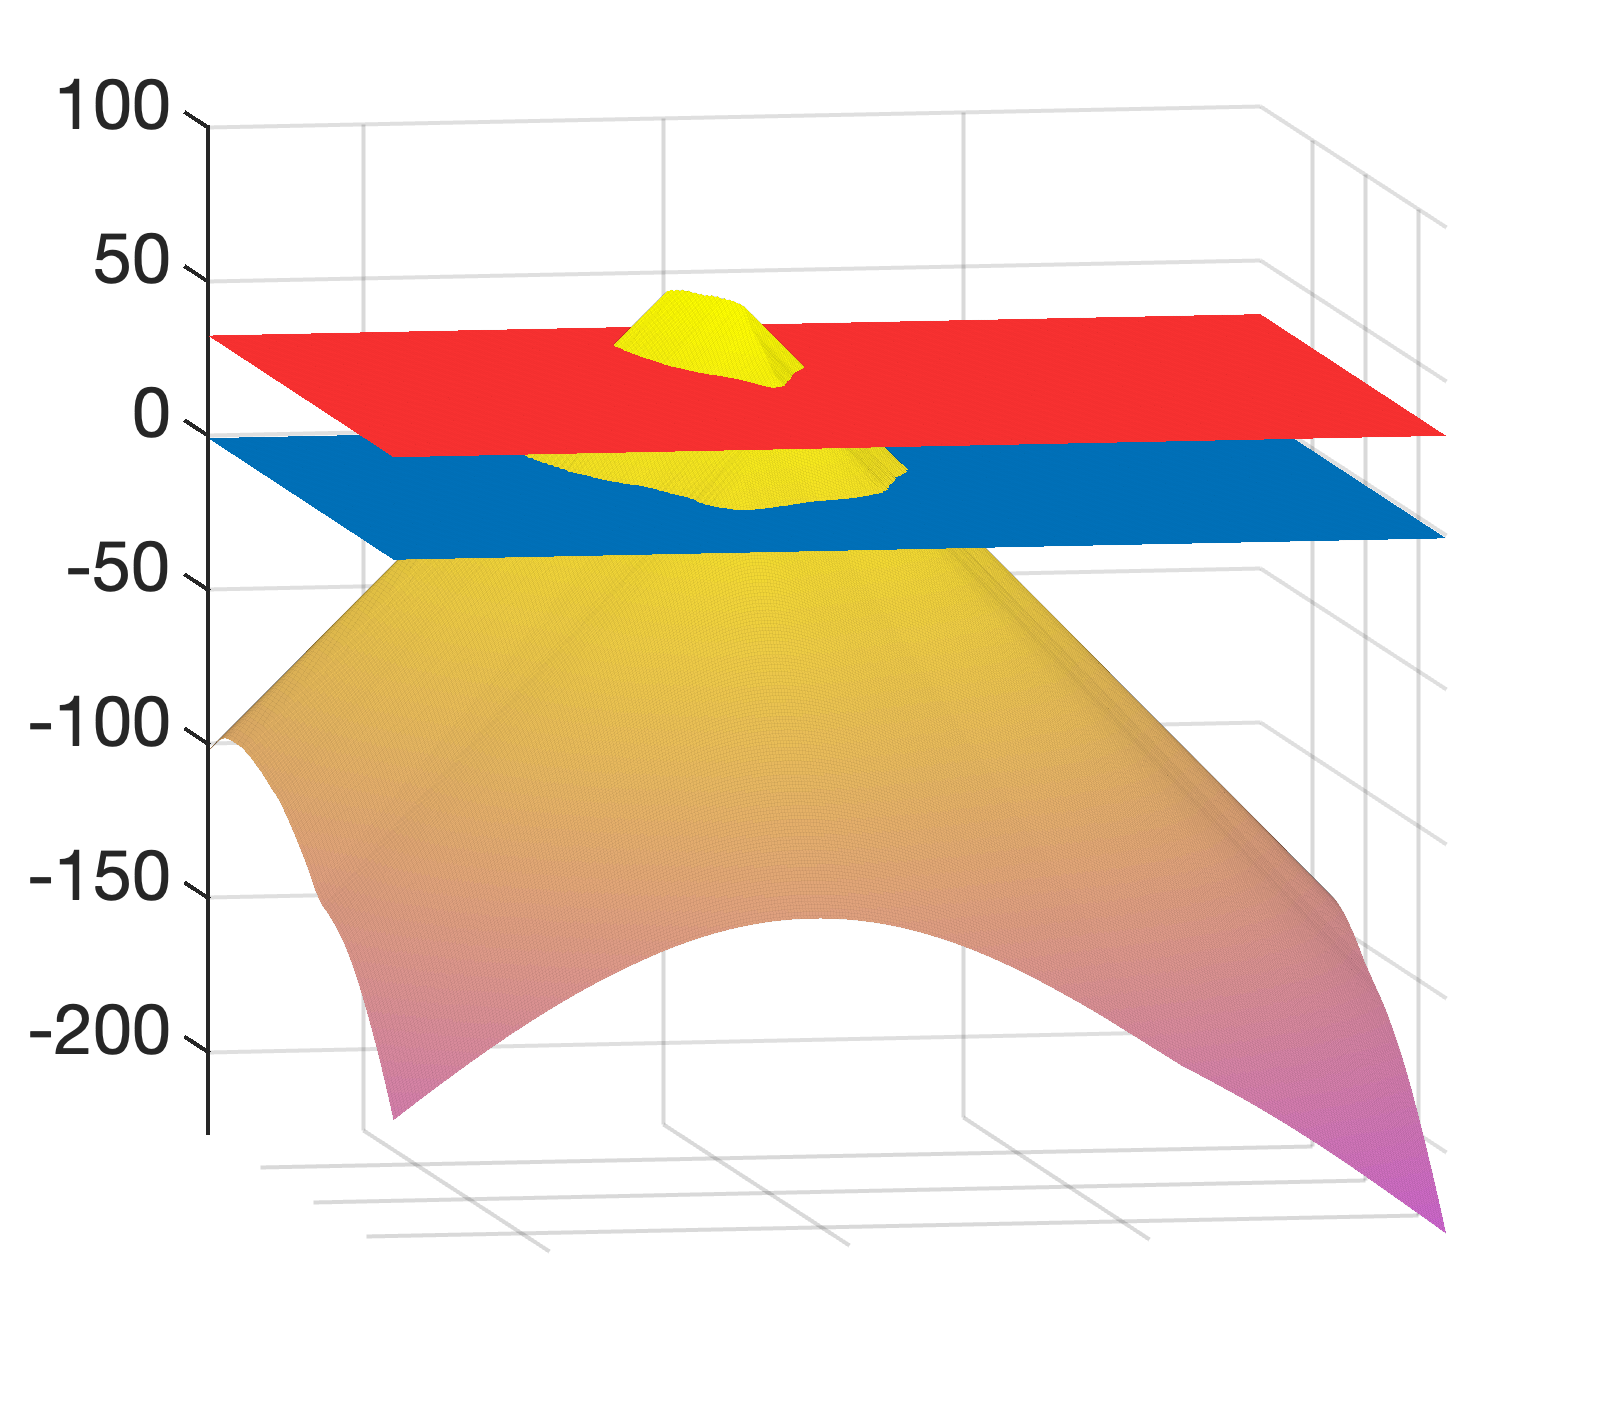
\includegraphics[width=0.24\textwidth]{../figures/learning/dist_surf/54.png}
		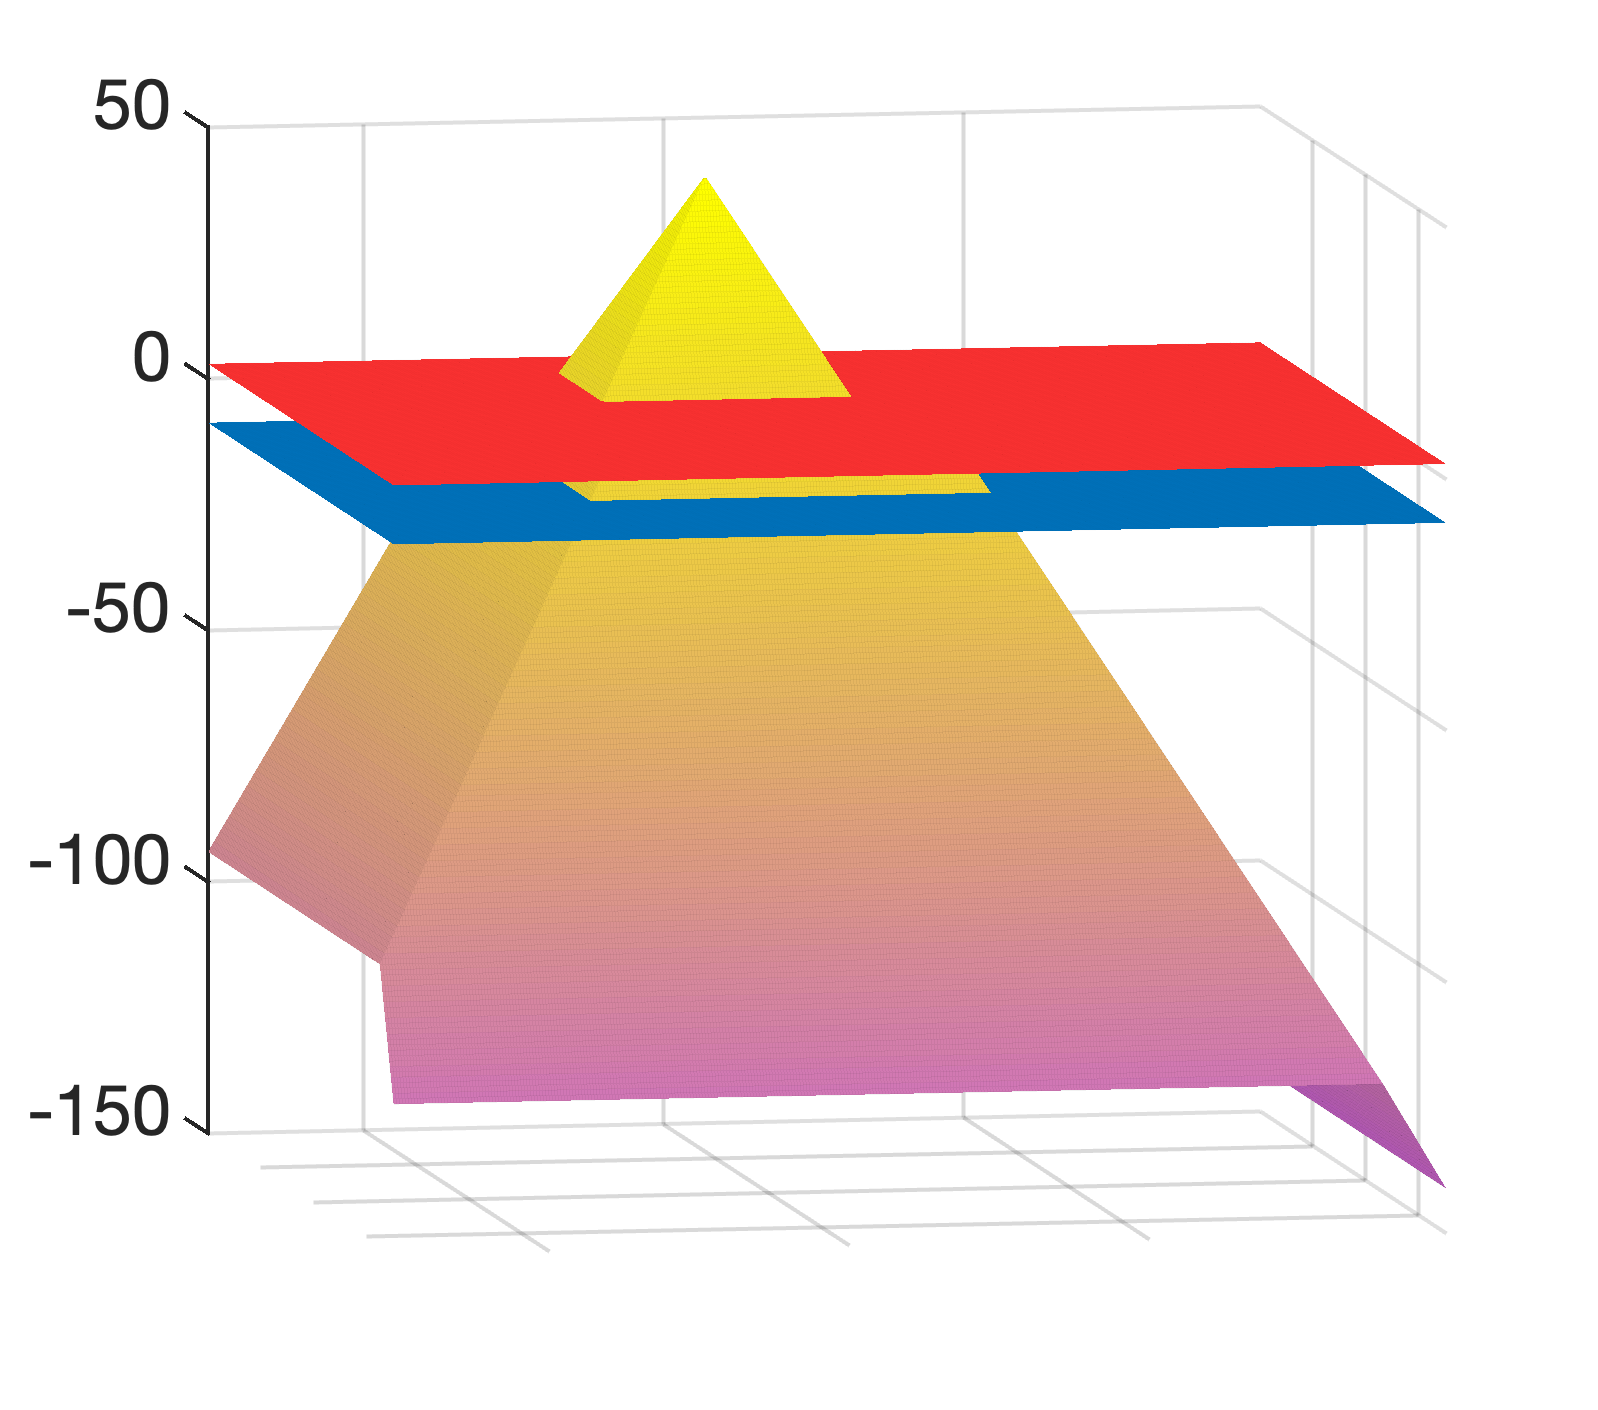
\includegraphics[width=0.24\textwidth]{../figures/learning/dist_bt_surf/54.png}\\
		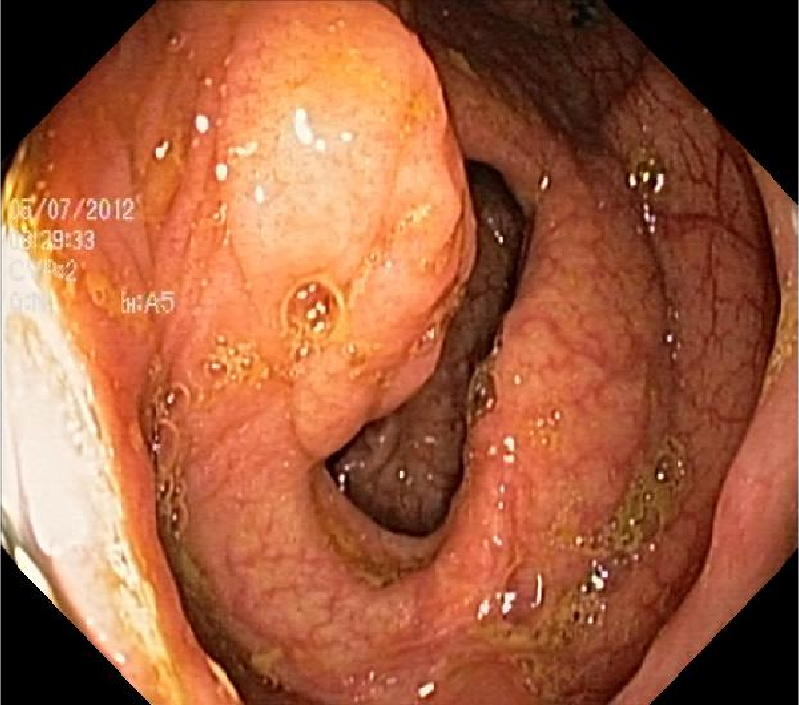
\includegraphics[width=0.24\textwidth]{../figures/learning/images/54.png}
		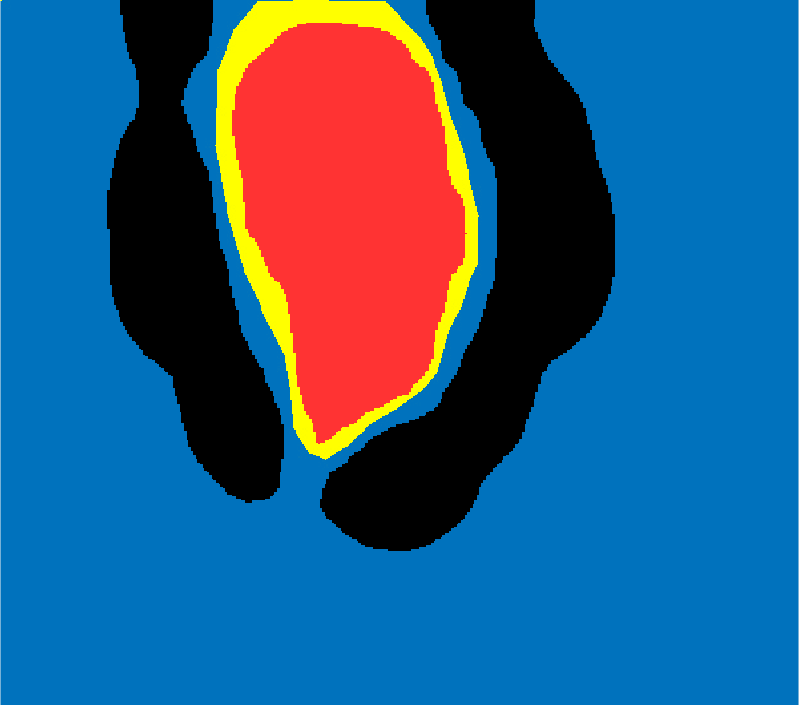
\includegraphics[width=0.24\textwidth]{../figures/learning/score_crs_marginal90/54.png}
		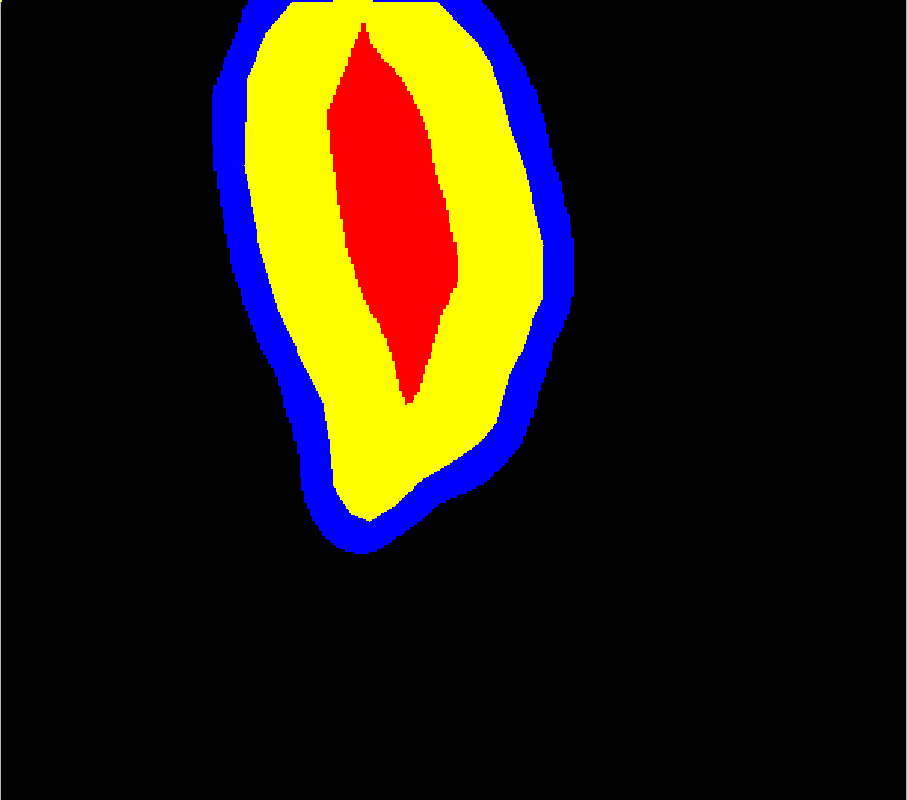
\includegraphics[width=0.24\textwidth]{../figures/learning/dist_crs_marginal90/54.png}
		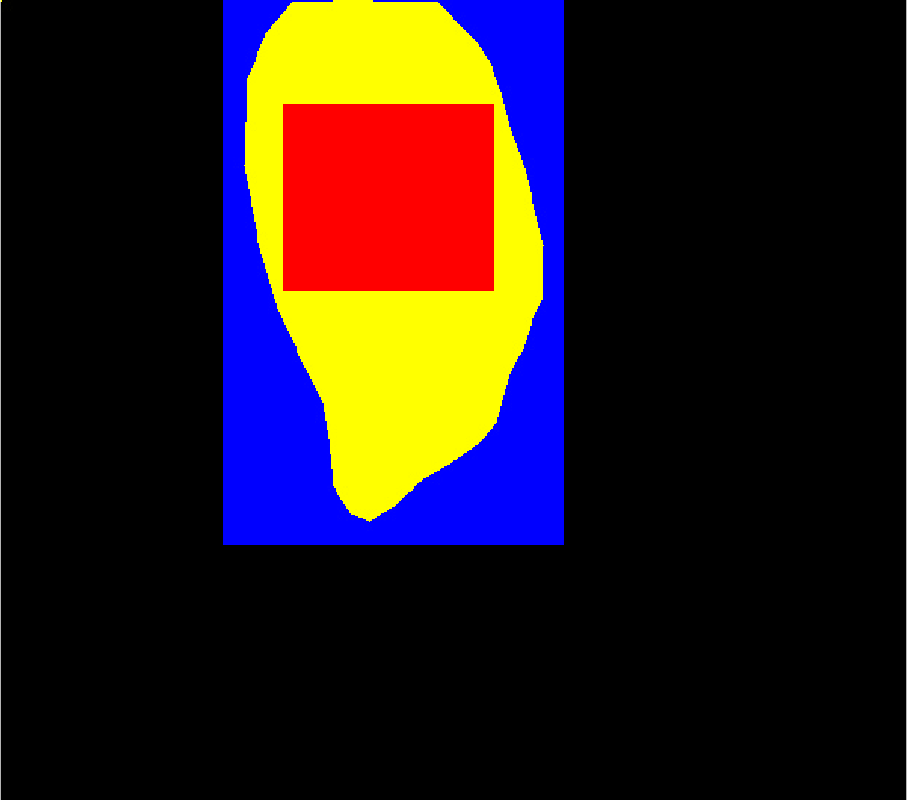
\includegraphics[width=0.24\textwidth]{../figures/learning/dist_bt_crs_marginal90/54.png}
	\end{center}
	\caption{Additional examples from the learning dataset. The layout of these figures is the same as for Figure \ref{fig:learning}.}
	\label{fig:learning2}
\end{figure}

\begin{figure}
	%	\centering
	\begin{center}
		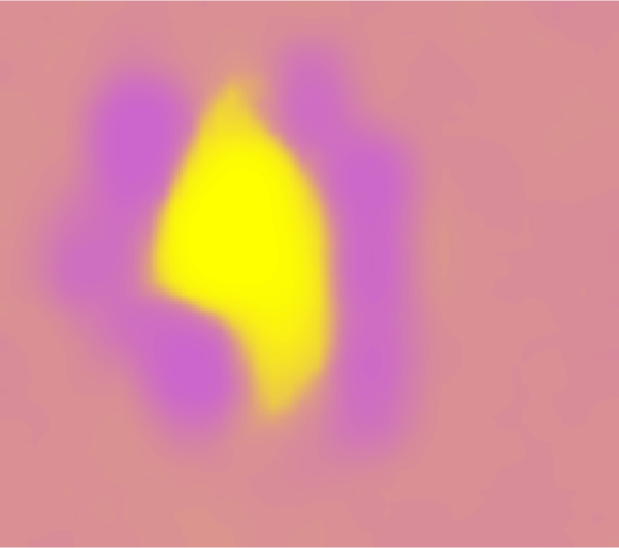
\includegraphics[width=0.24\textwidth]{../figures/learning/scores/183.png}
		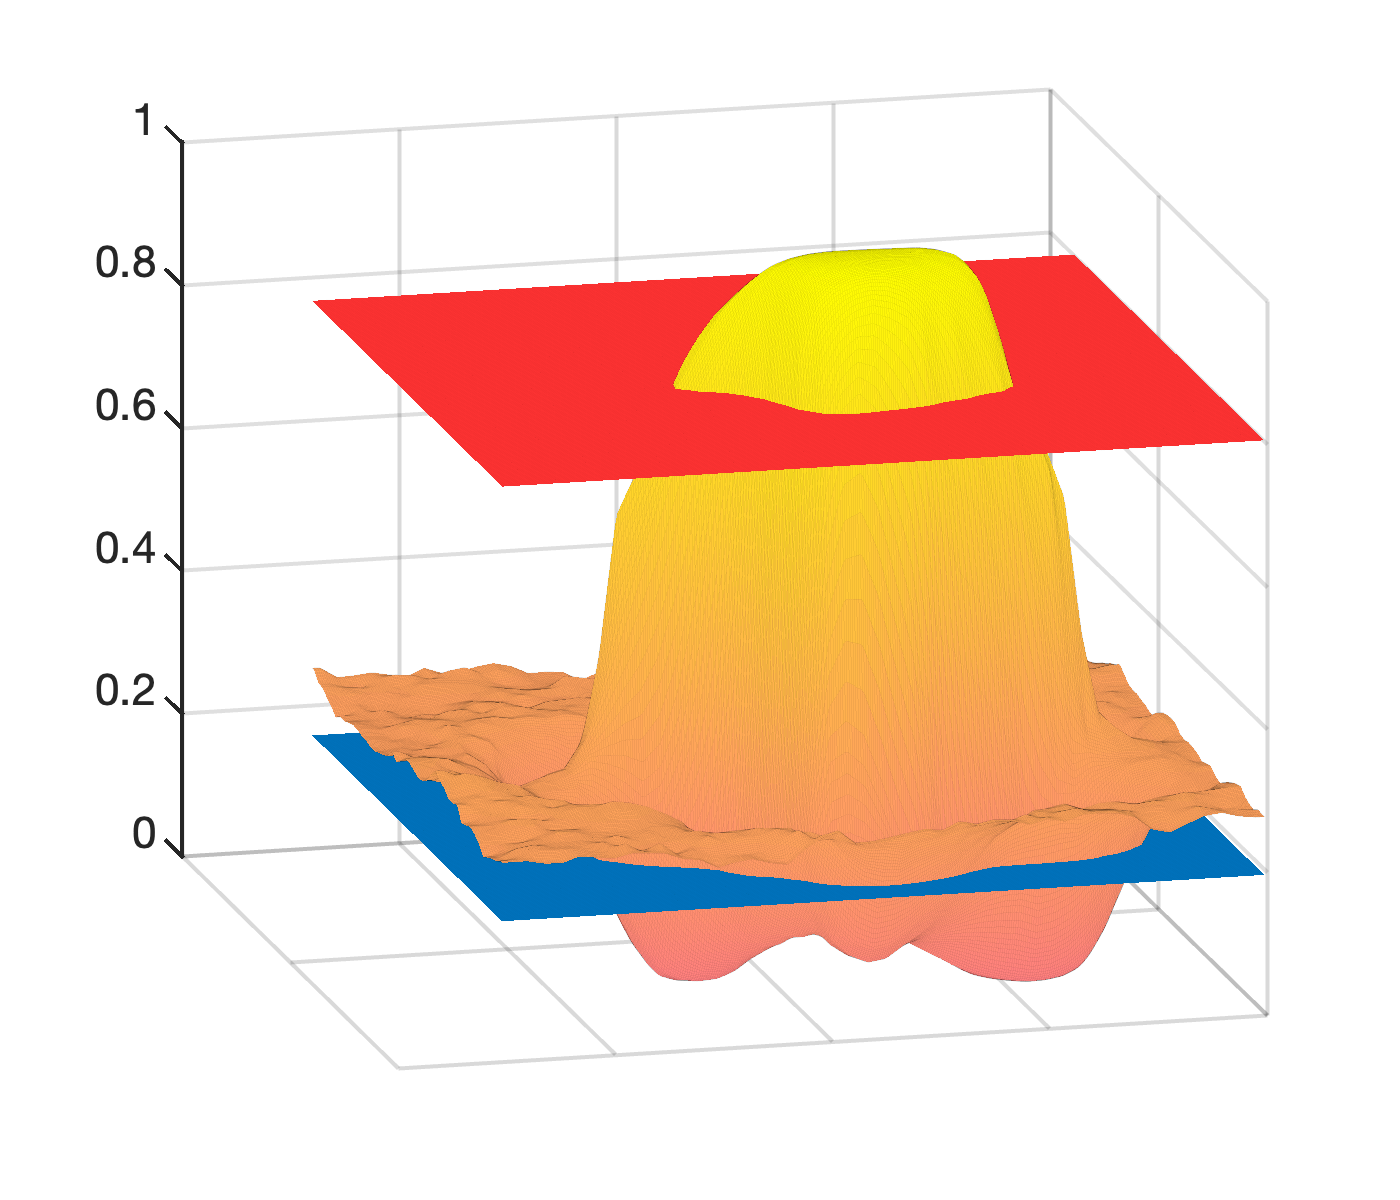
\includegraphics[width=0.24\textwidth]{../figures/learning/score_surf/183.png}	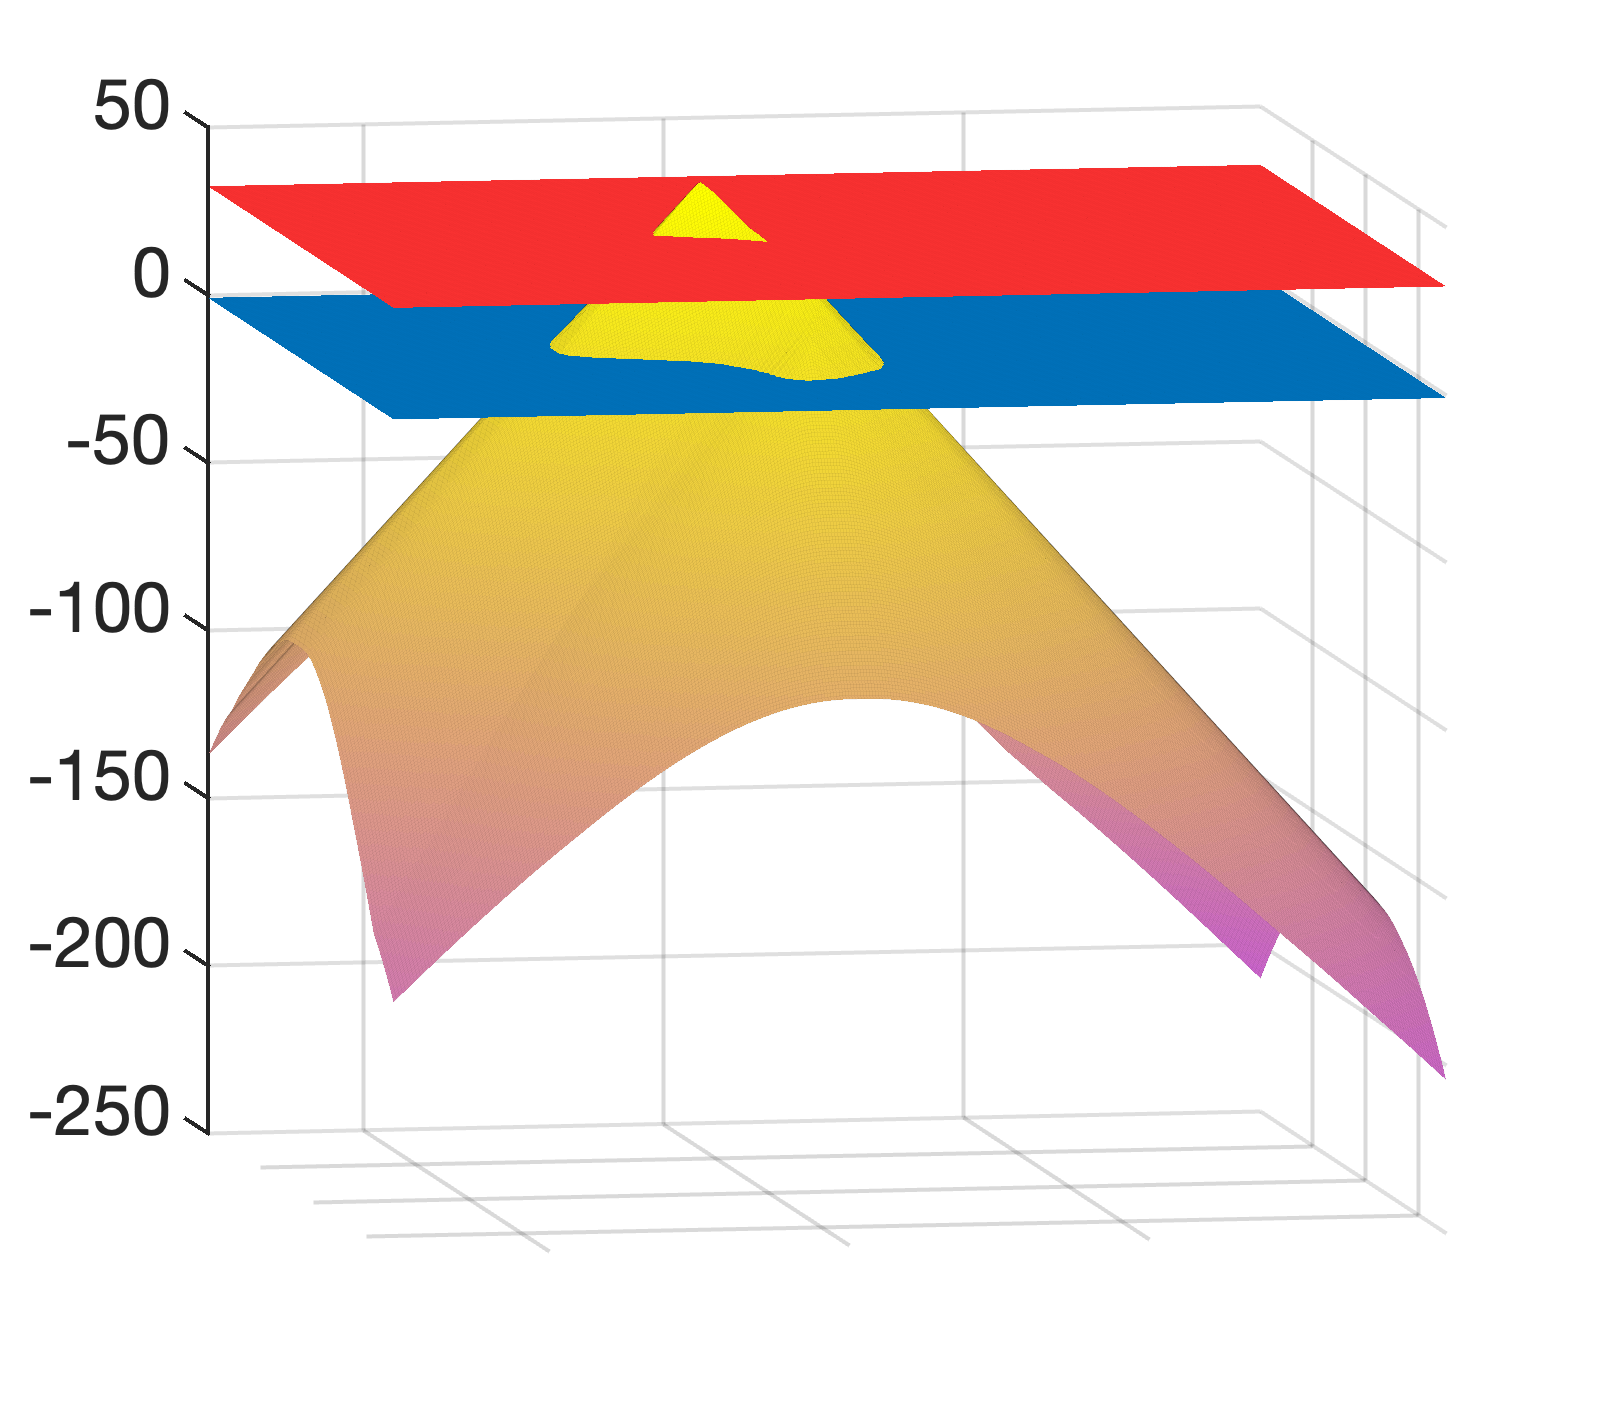
\includegraphics[width=0.24\textwidth]{../figures/learning/dist_surf/183.png}
		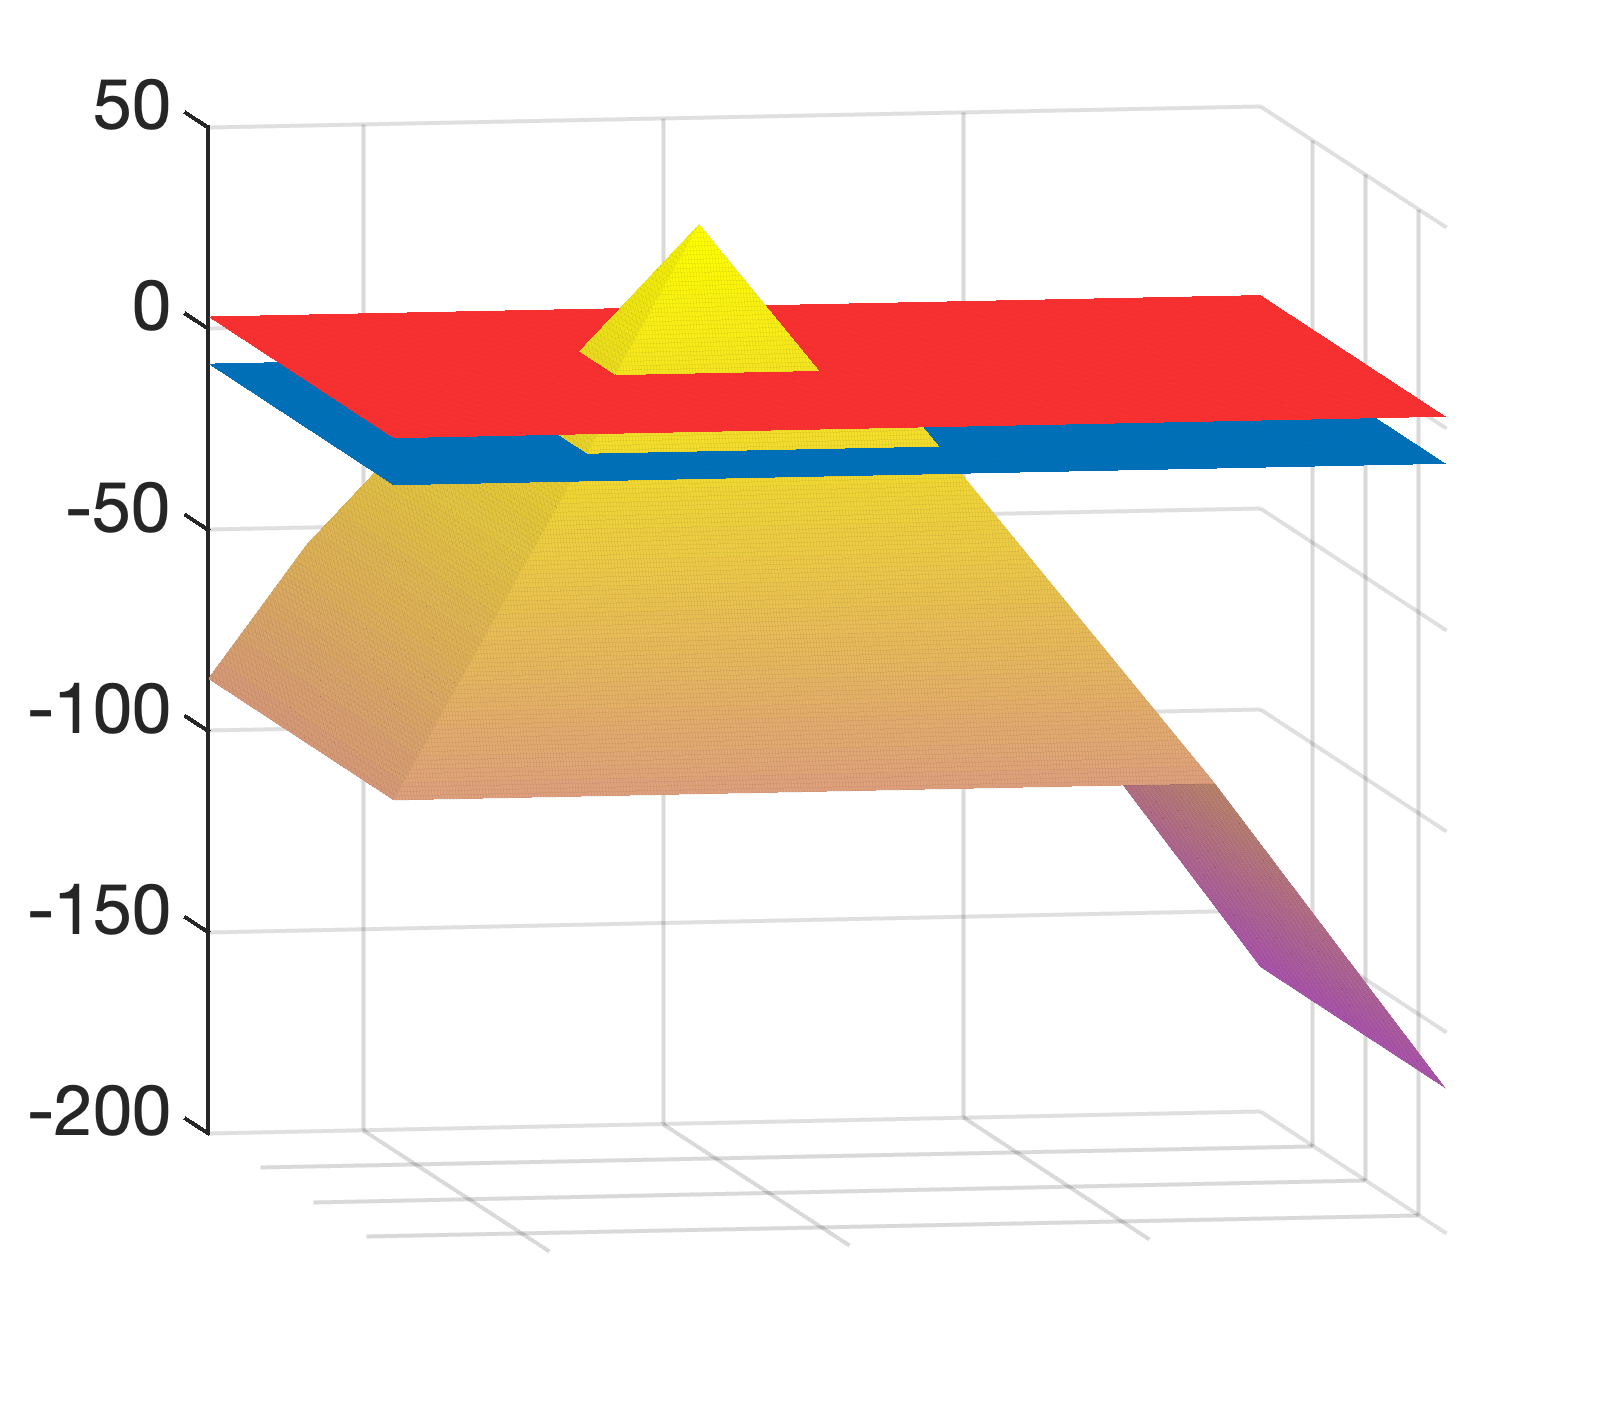
\includegraphics[width=0.24\textwidth]{../figures/learning/dist_bt_surf/183.png}\\
		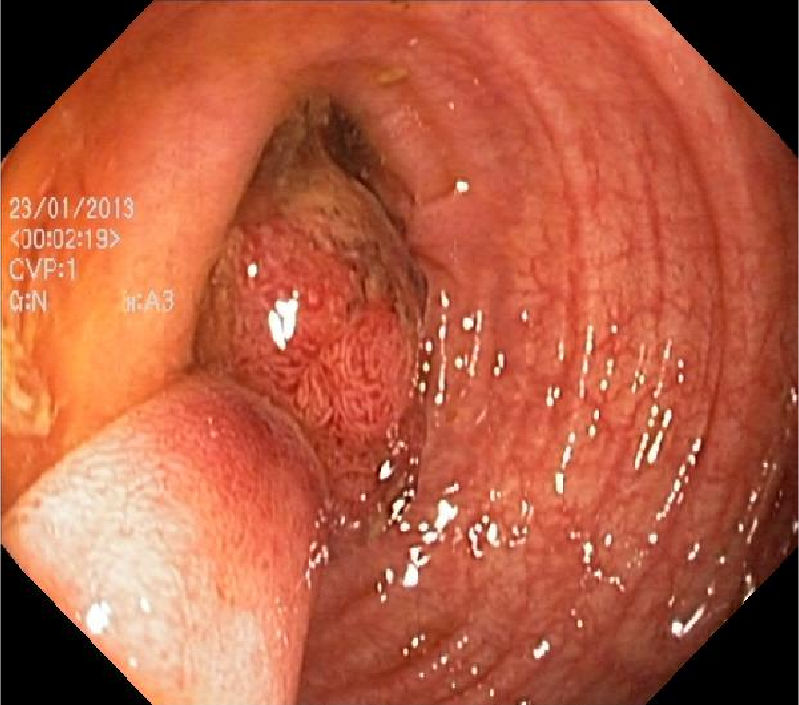
\includegraphics[width=0.24\textwidth]{../figures/learning/images/183.png}
		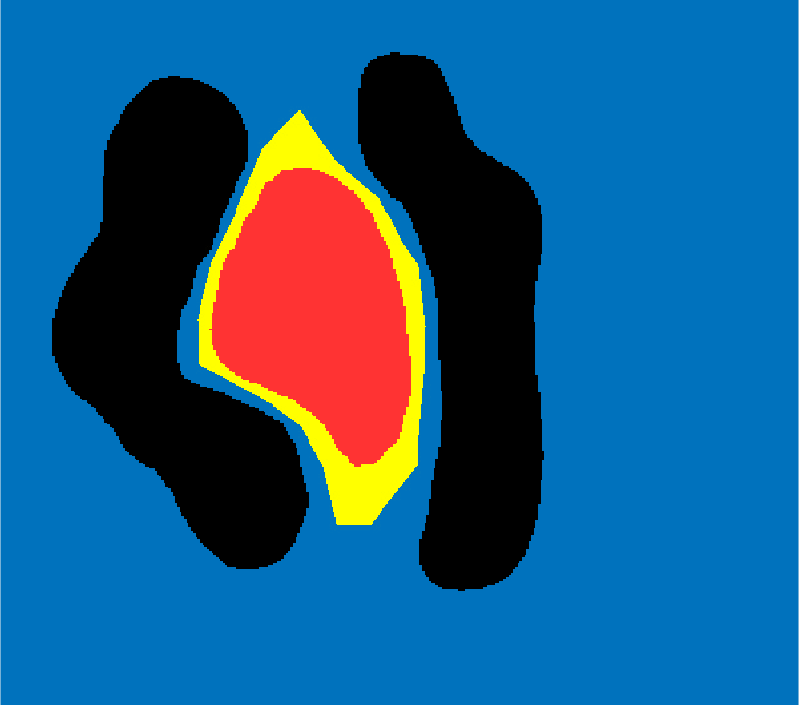
\includegraphics[width=0.24\textwidth]{../figures/learning/score_crs_marginal90/183.png}
		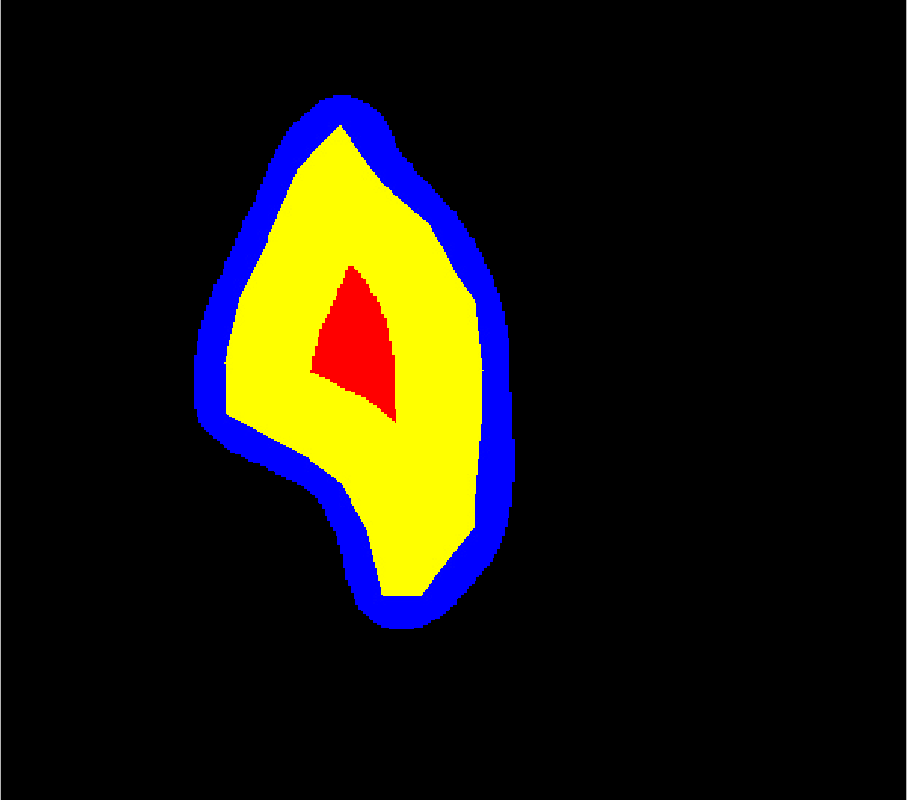
\includegraphics[width=0.24\textwidth]{../figures/learning/dist_crs_marginal90/183.png}
		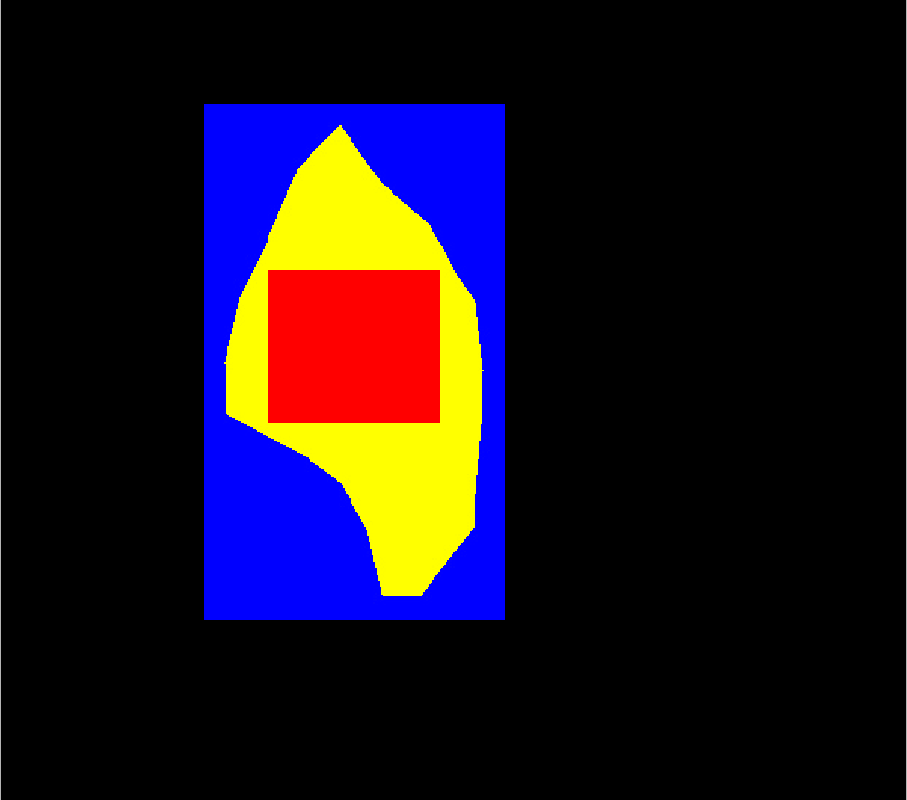
\includegraphics[width=0.24\textwidth]{../figures/learning/dist_bt_crs_marginal90/183.png}\\
		\vspace{0.5cm}
		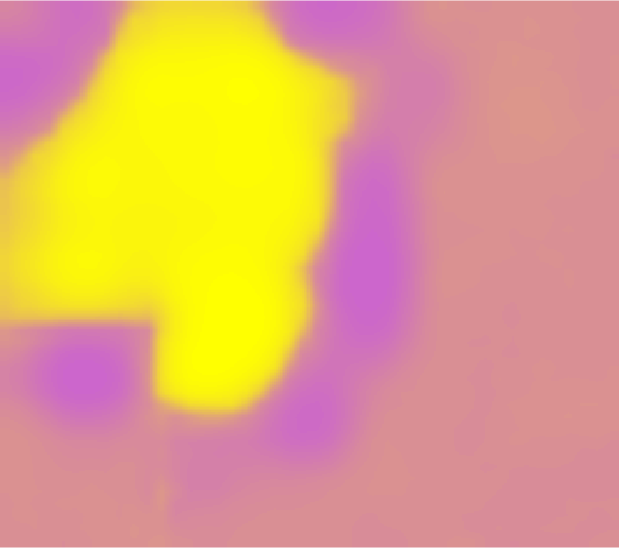
\includegraphics[width=0.24\textwidth]{../figures/learning/scores/530.png}
		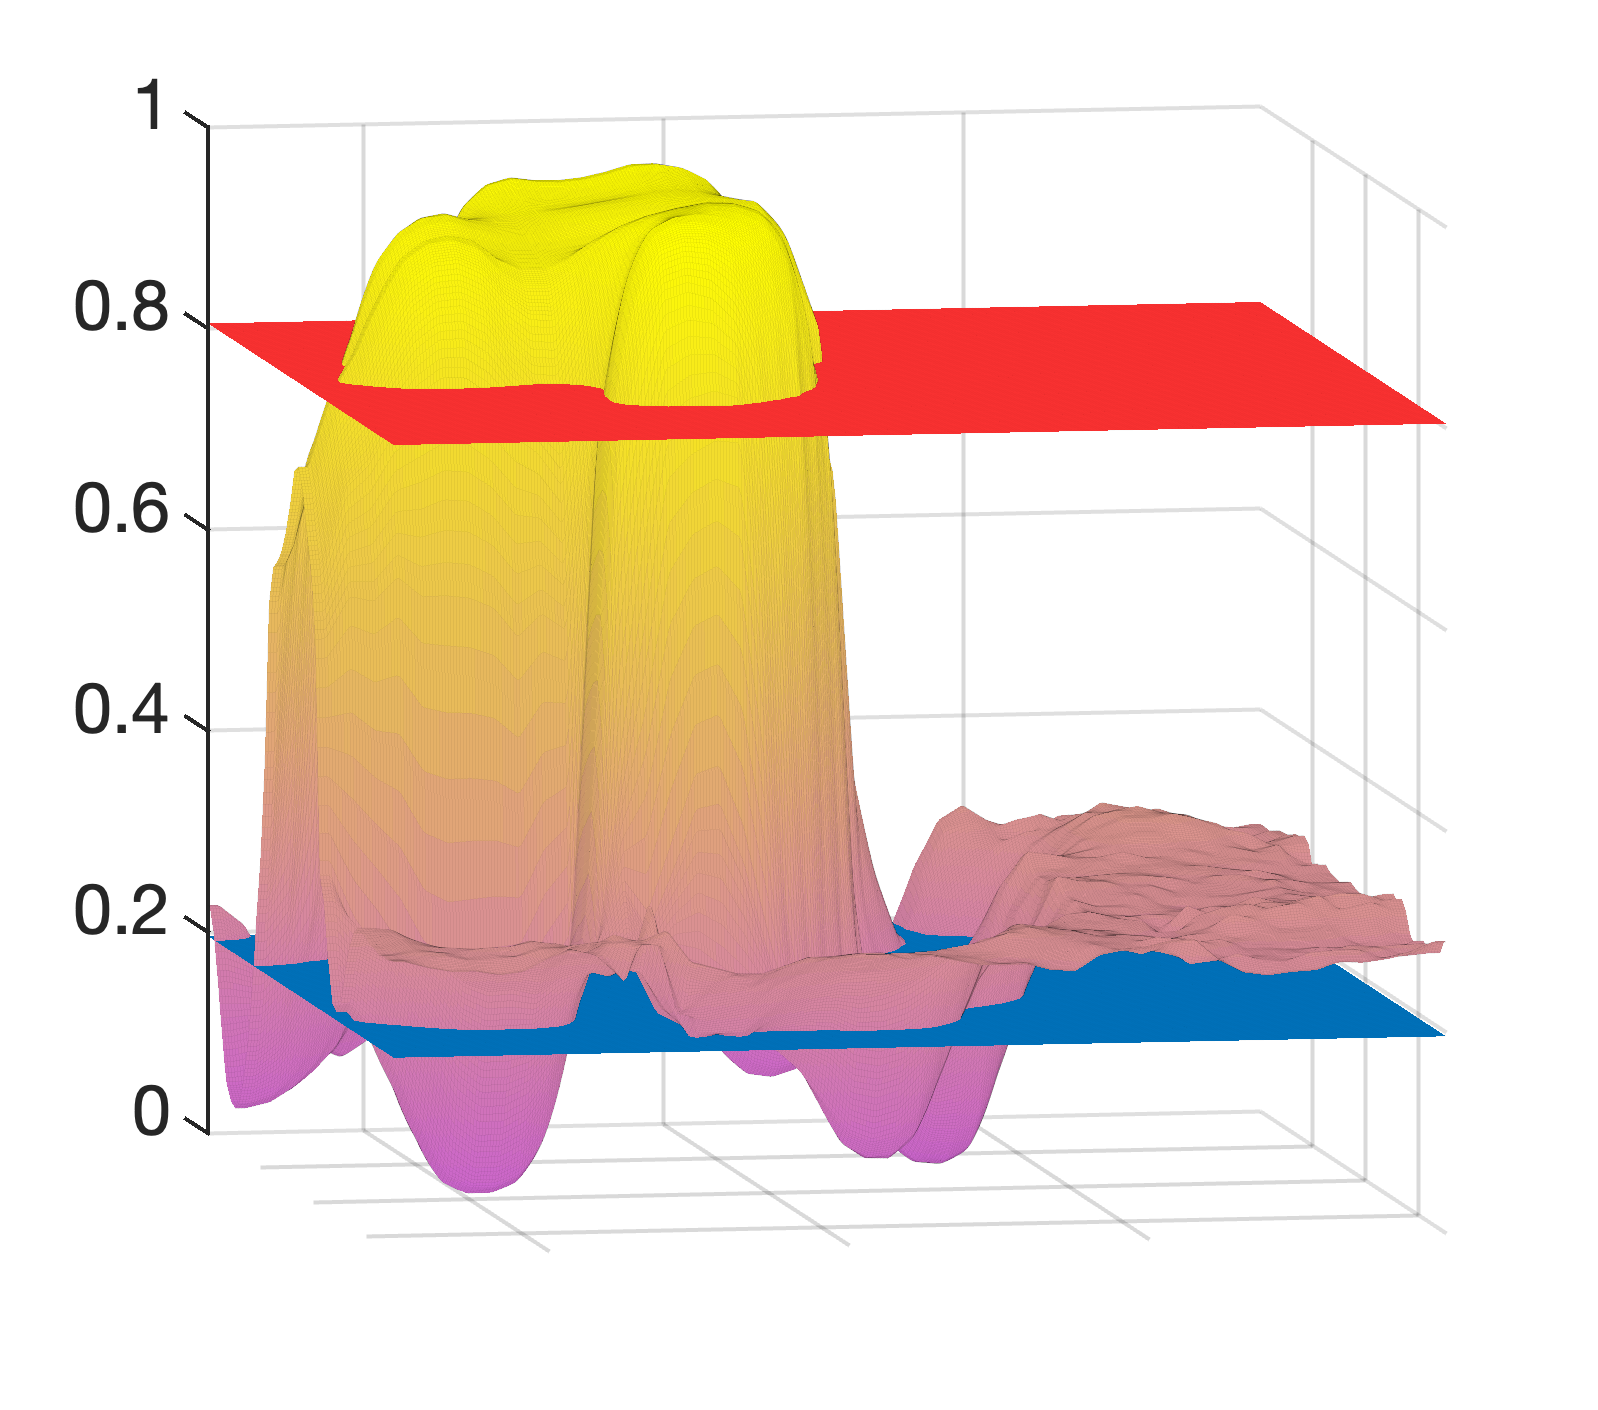
\includegraphics[width=0.24\textwidth]{../figures/learning/score_surf/530.png}	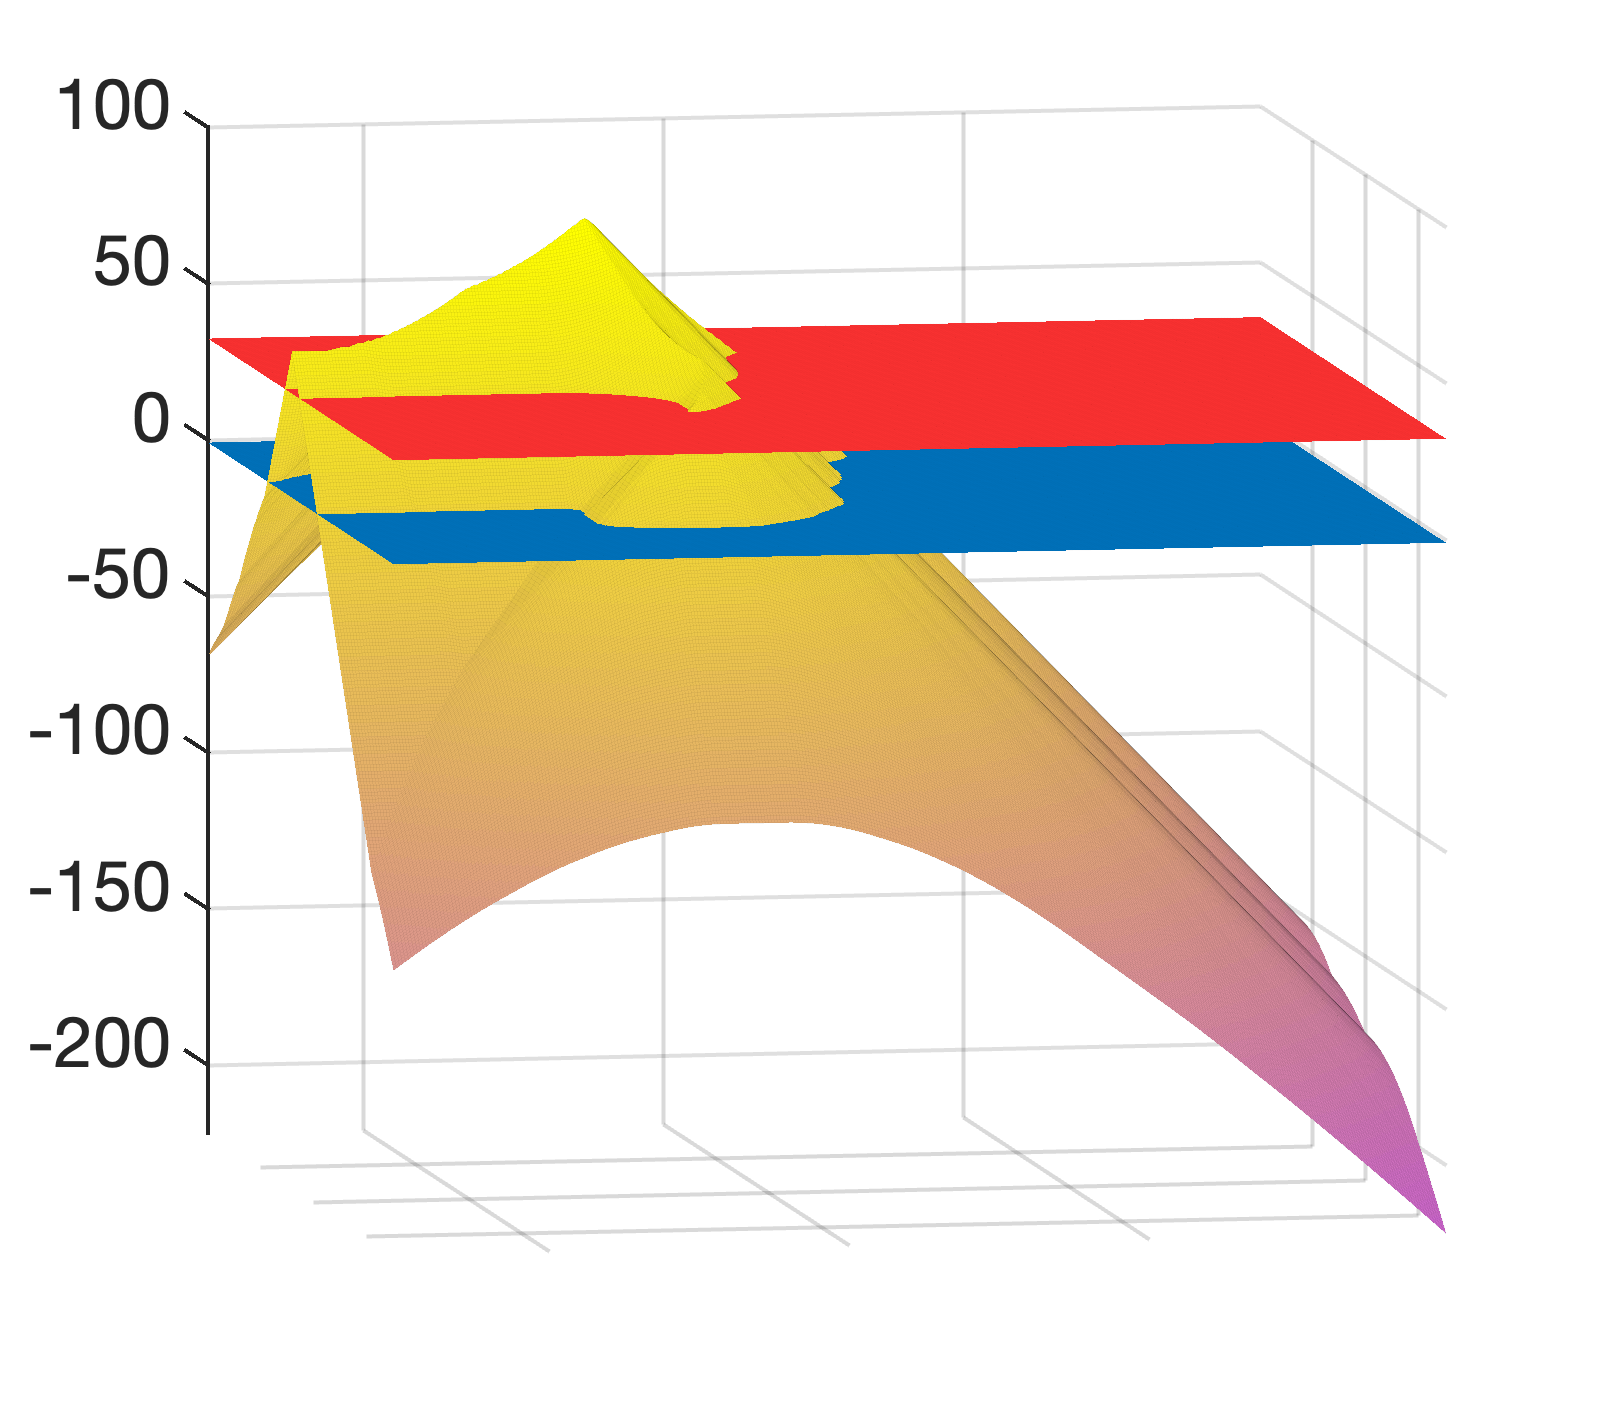
\includegraphics[width=0.24\textwidth]{../figures/learning/dist_surf/530.png}
		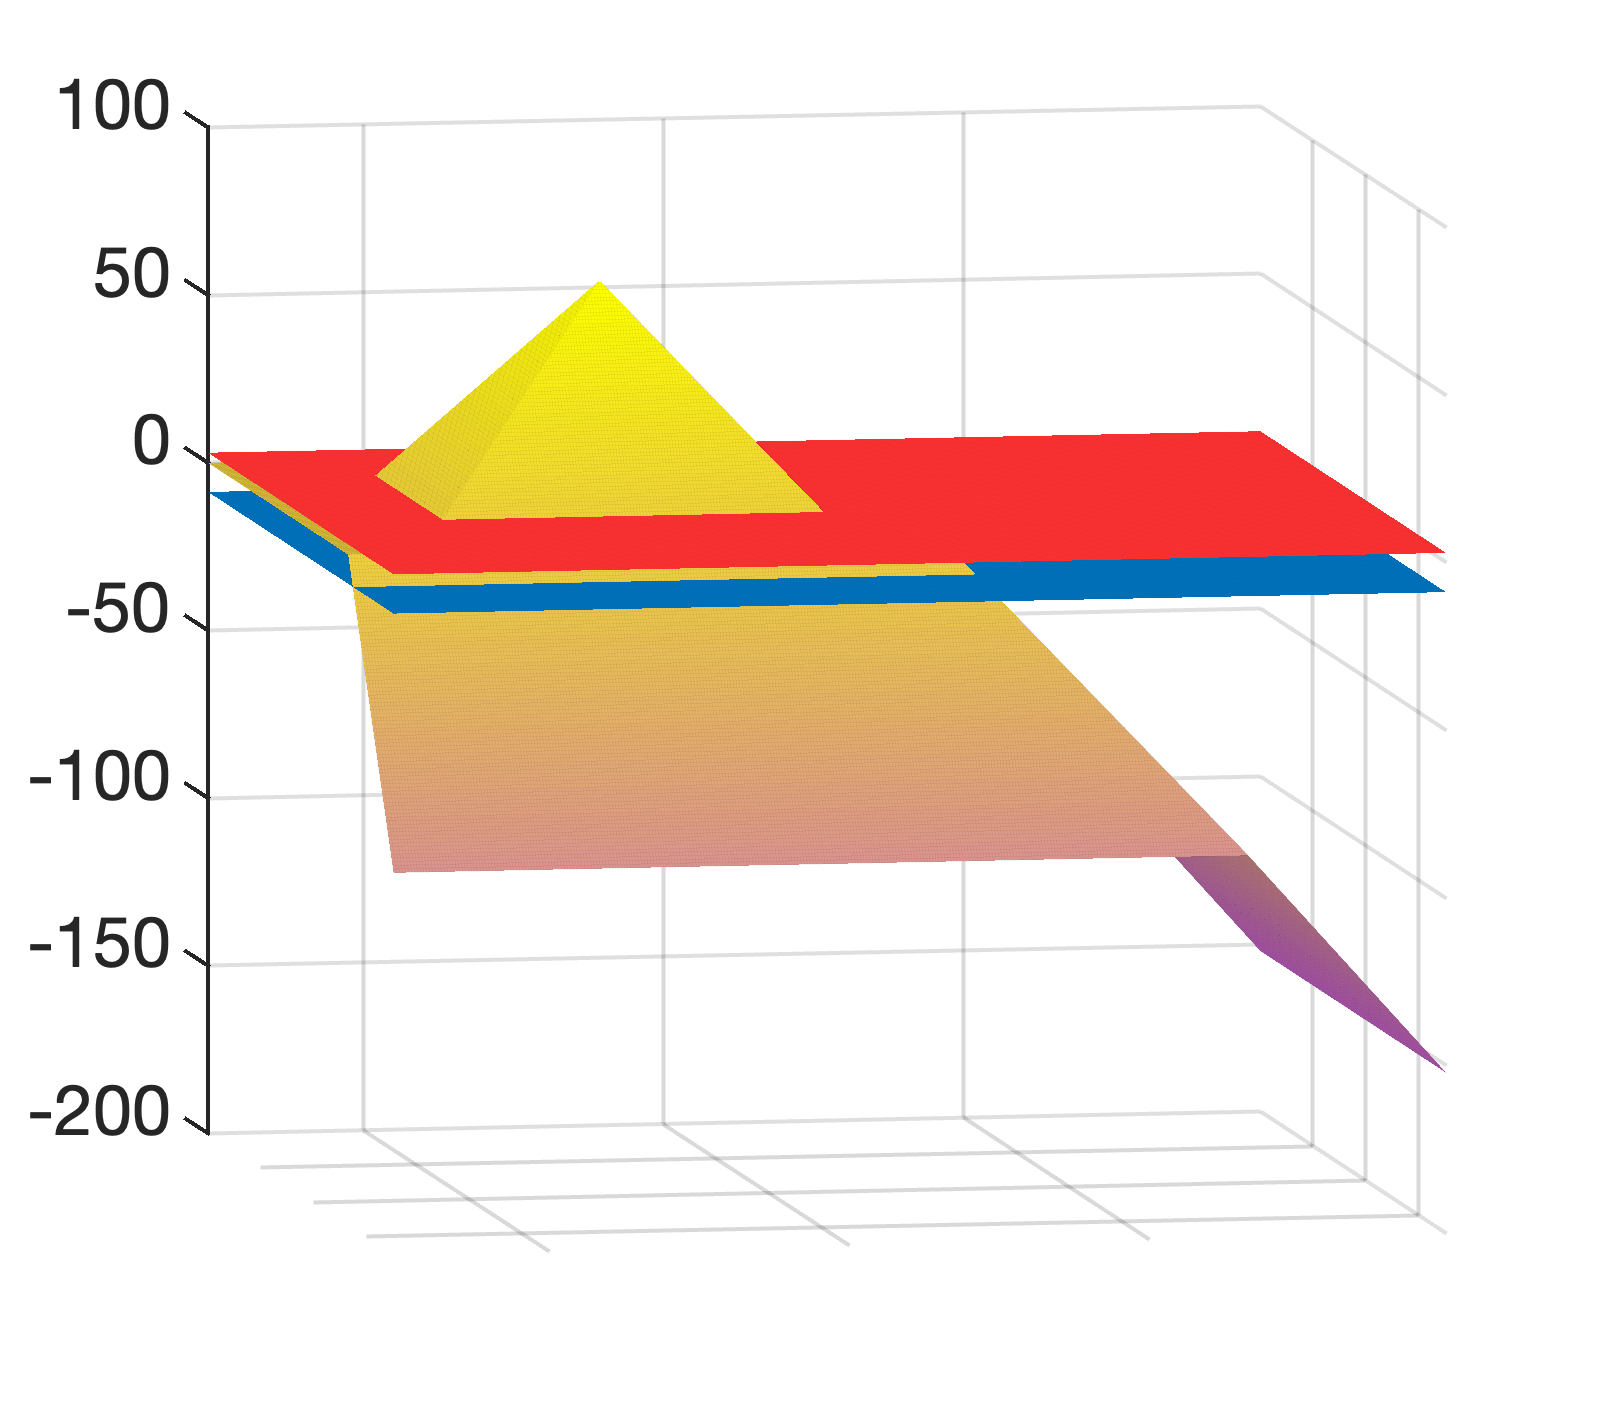
\includegraphics[width=0.24\textwidth]{../figures/learning/dist_bt_surf/530.png}\\
		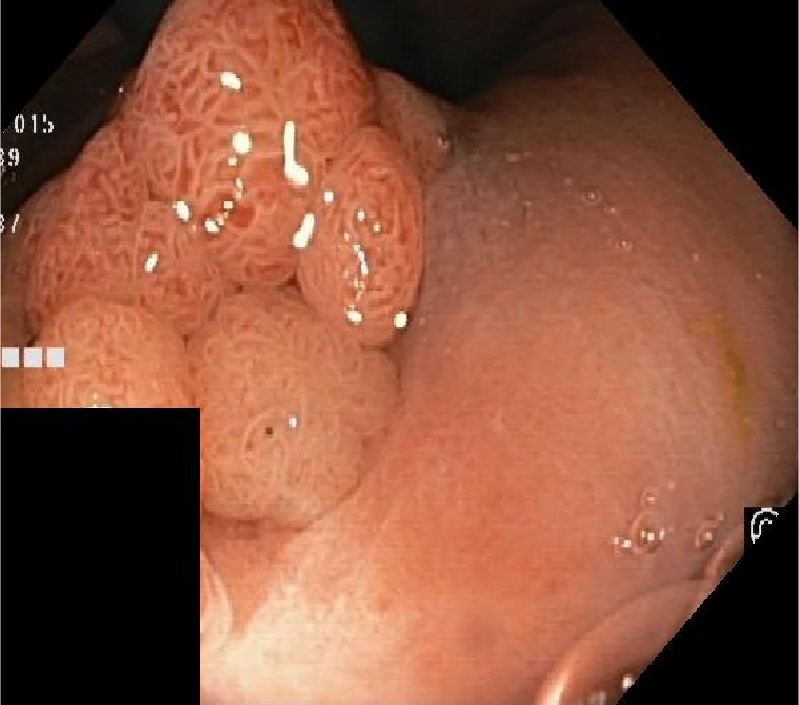
\includegraphics[width=0.24\textwidth]{../figures/learning/images/530.png}
		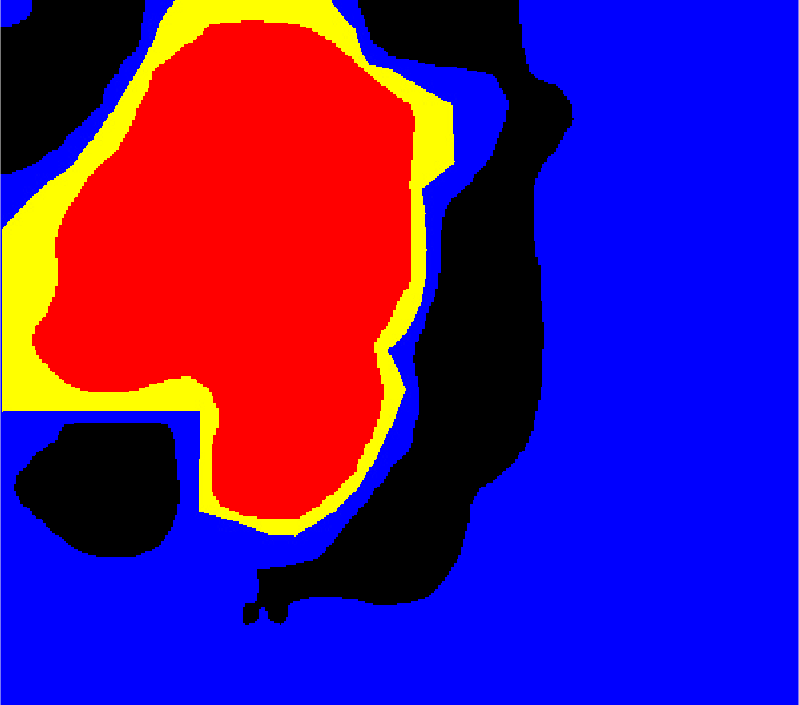
\includegraphics[width=0.24\textwidth]{../figures/learning/score_crs_marginal90/530.png}
		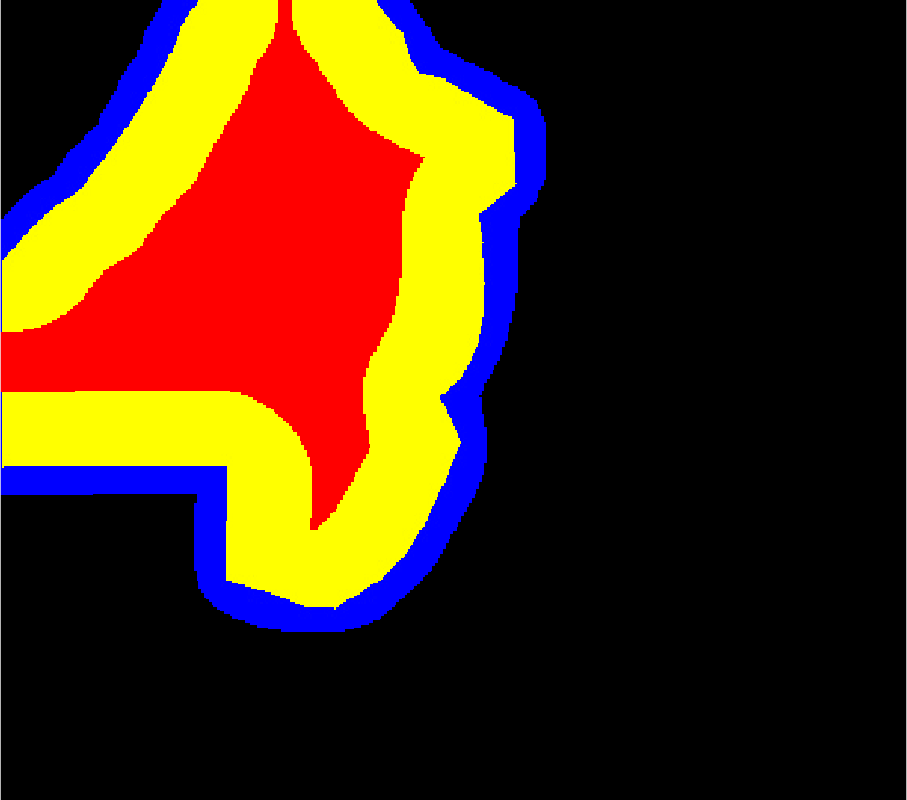
\includegraphics[width=0.24\textwidth]{../figures/learning/dist_crs_marginal90/530.png}
		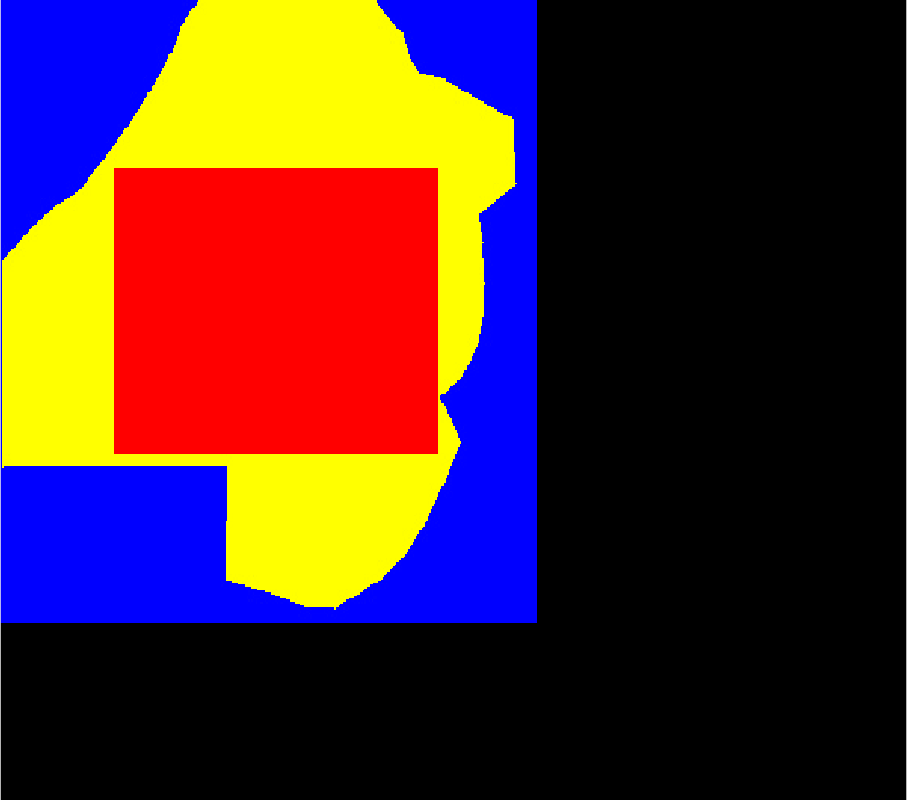
\includegraphics[width=0.24\textwidth]{../figures/learning/dist_bt_crs_marginal90/530.png}\\
		\vspace{0.5cm}
		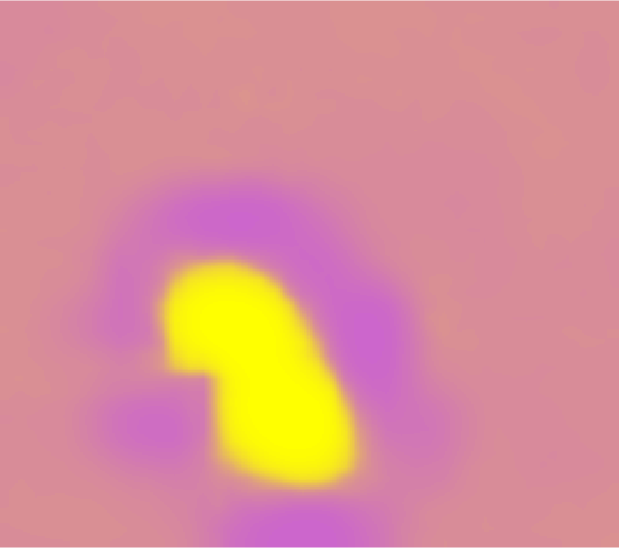
\includegraphics[width=0.24\textwidth]{../figures/learning/scores/754.png}
		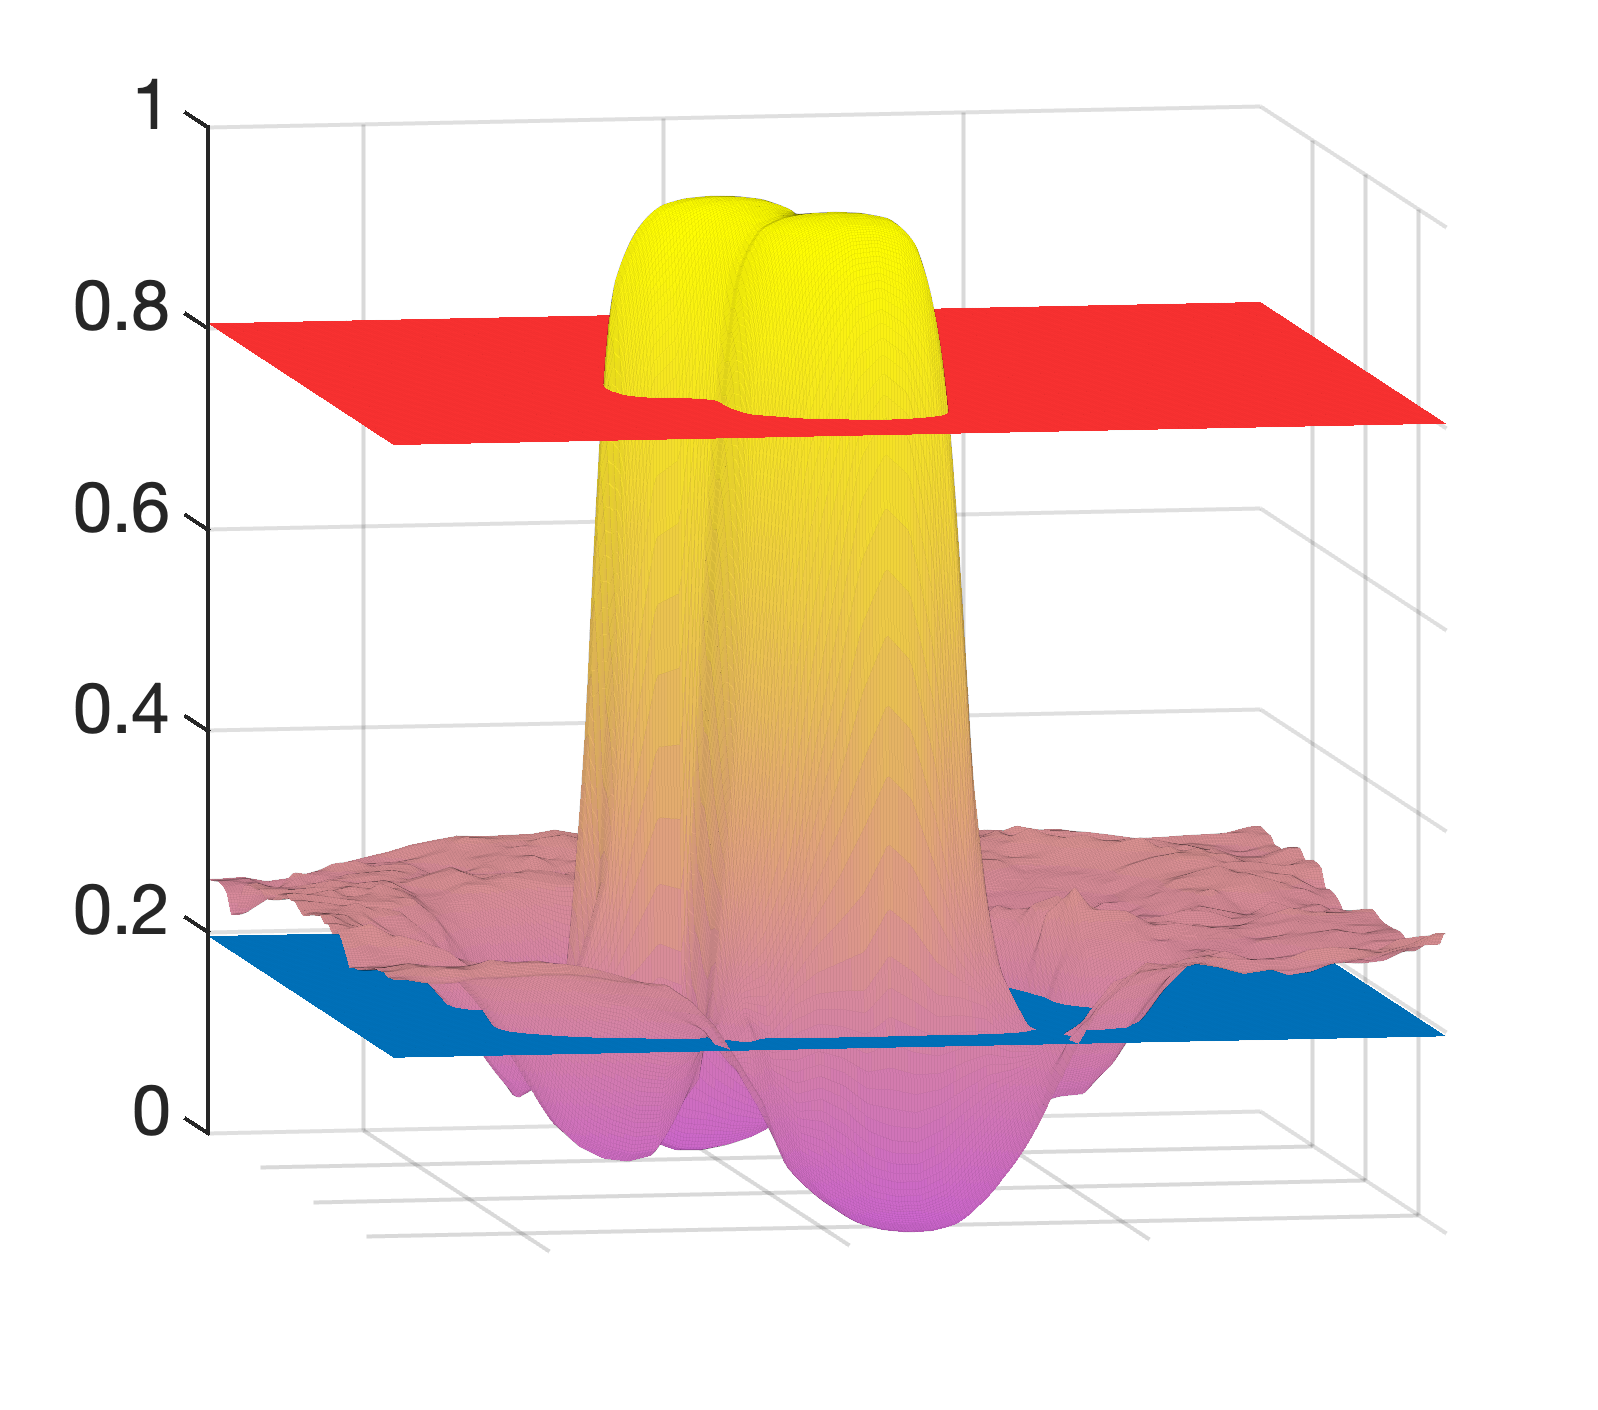
\includegraphics[width=0.24\textwidth]{../figures/learning/score_surf/754.png}	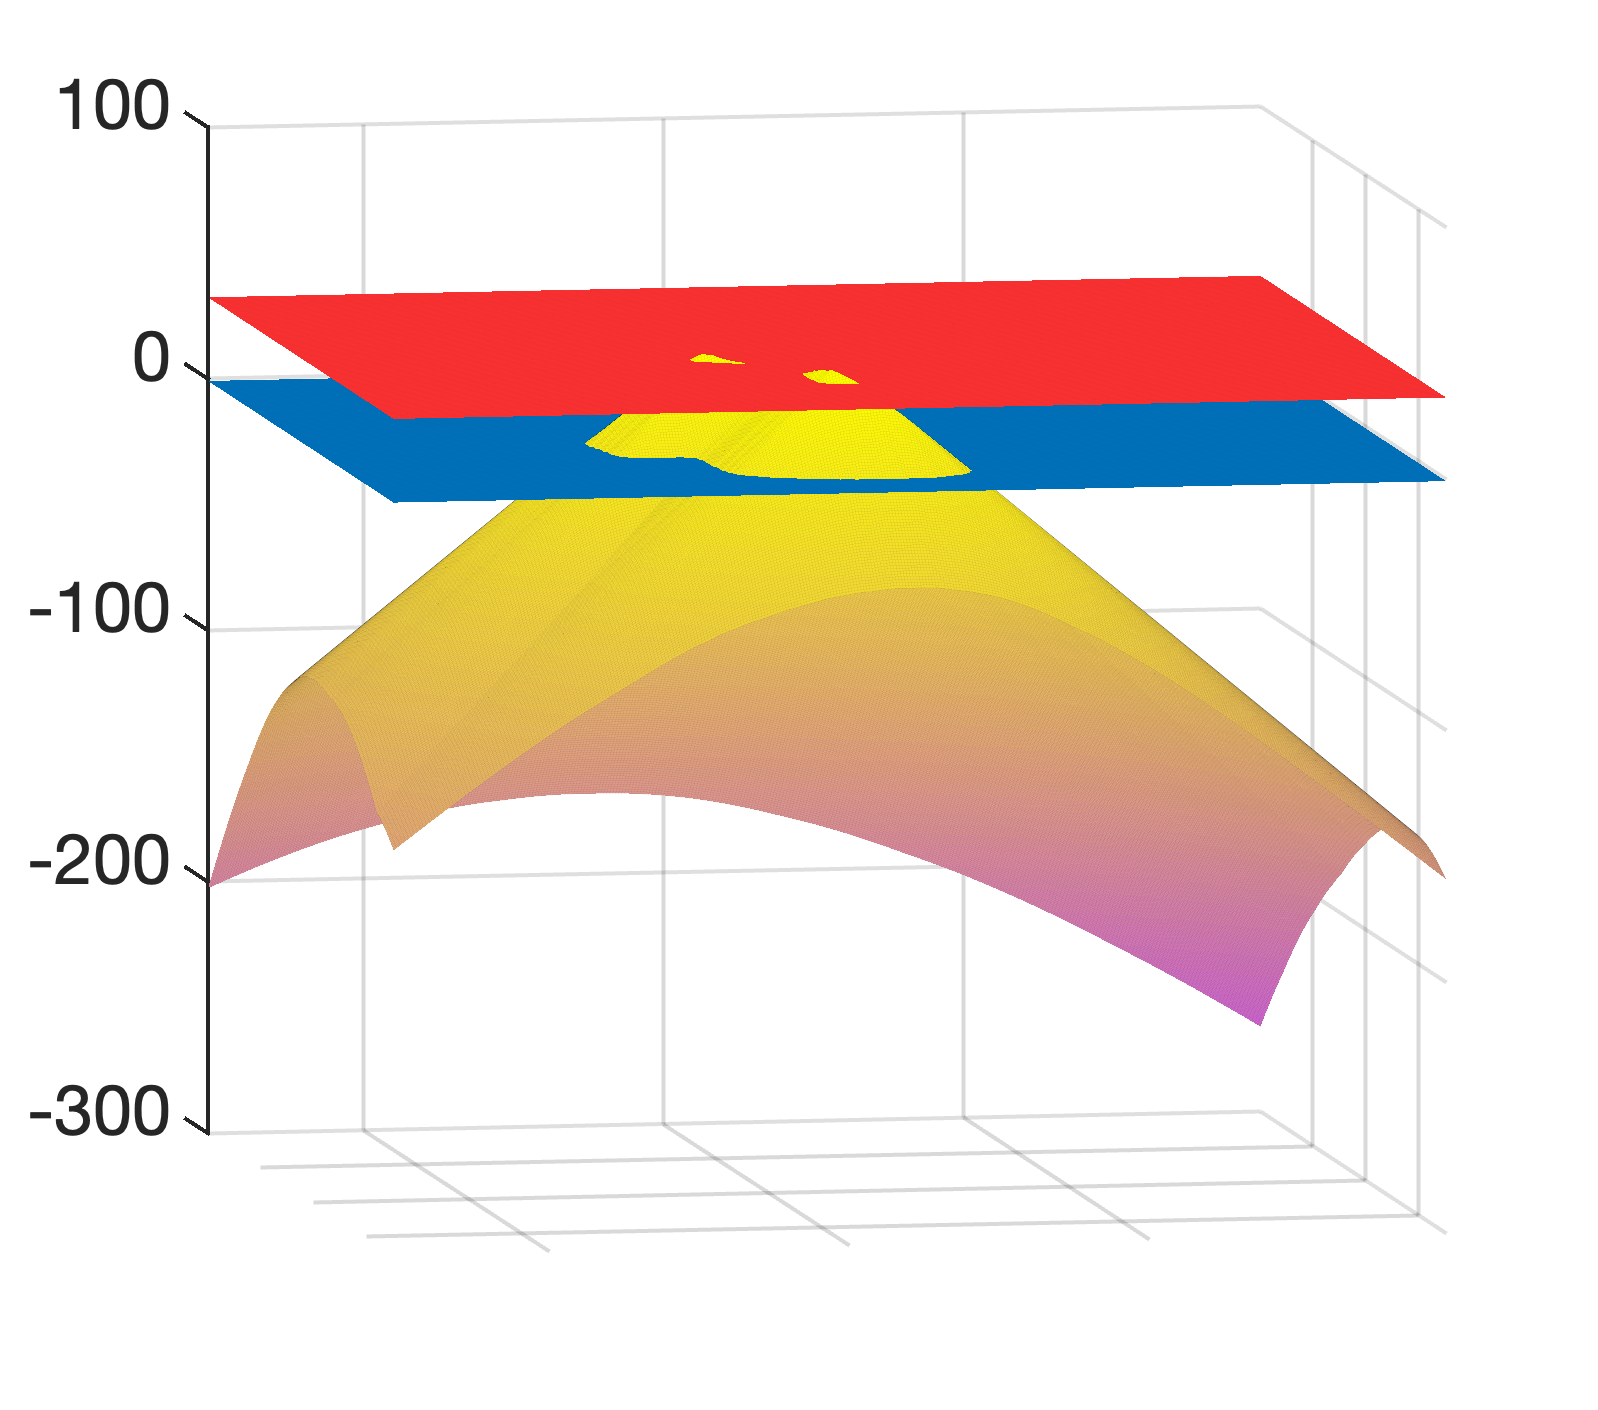
\includegraphics[width=0.24\textwidth]{../figures/learning/dist_surf/754.png}
		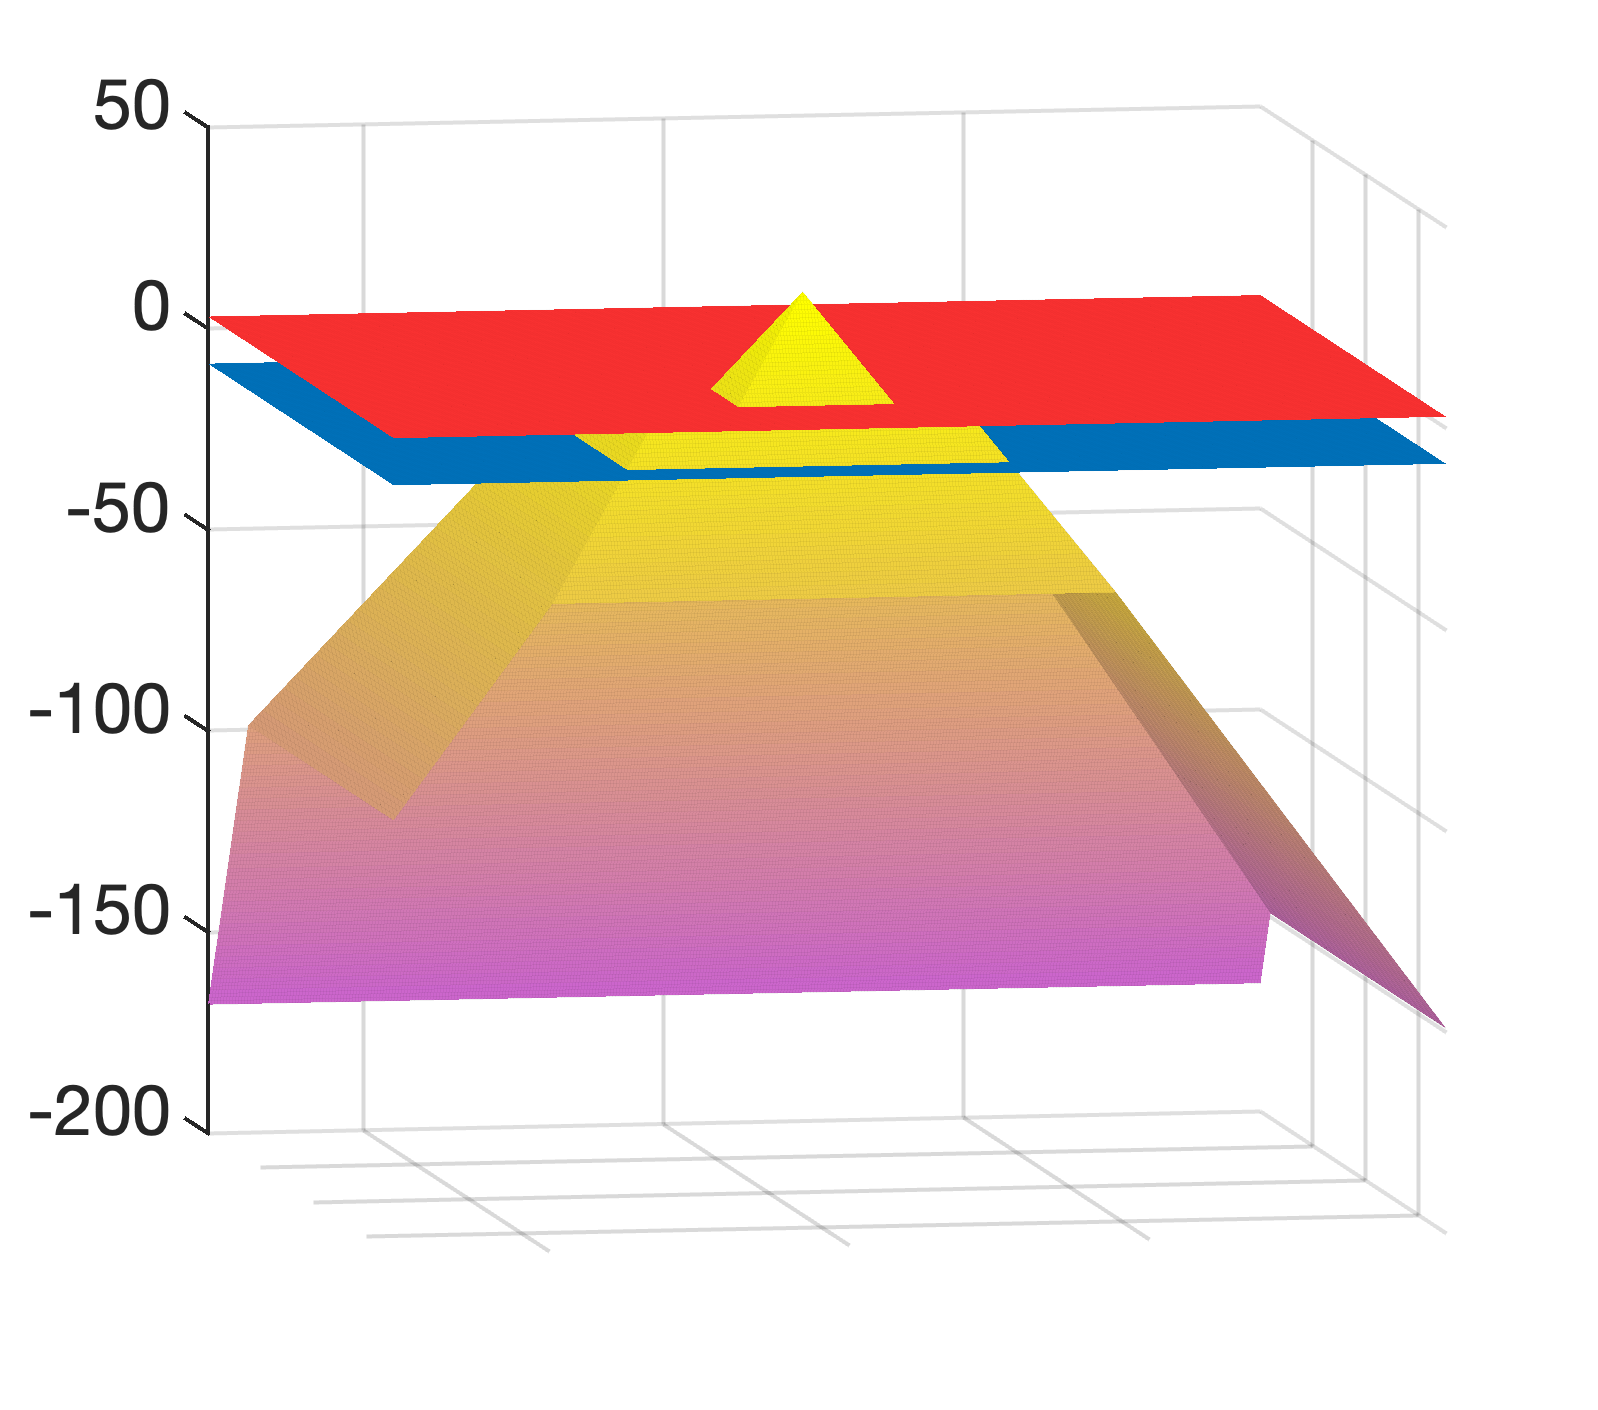
\includegraphics[width=0.24\textwidth]{../figures/learning/dist_bt_surf/754.png}\\
		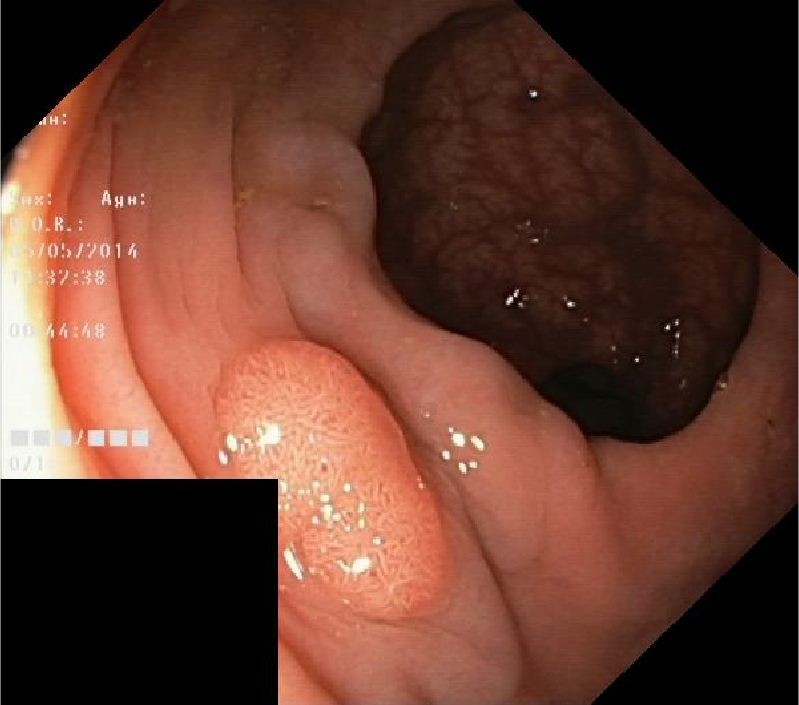
\includegraphics[width=0.24\textwidth]{../figures/learning/images/754.png}
		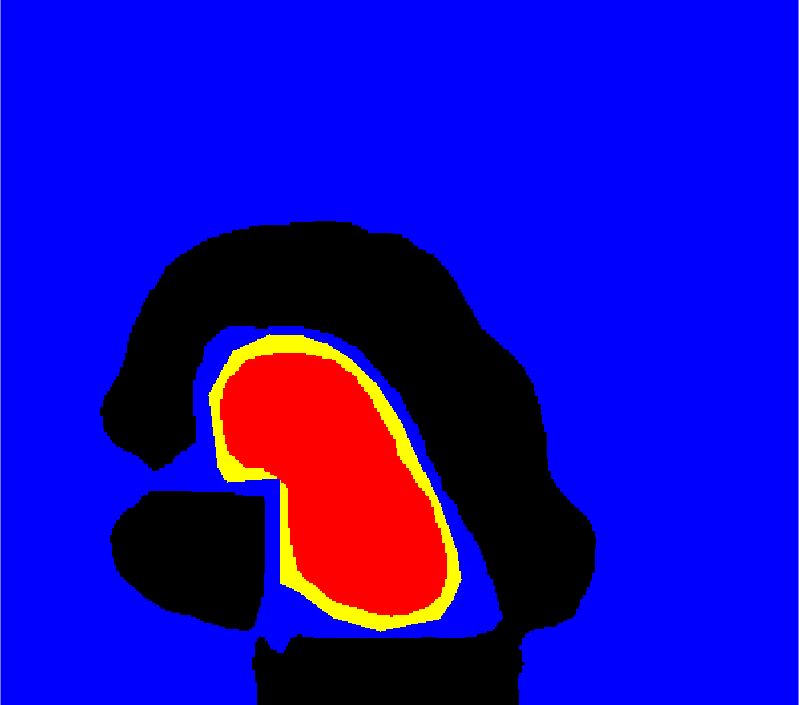
\includegraphics[width=0.24\textwidth]{../figures/learning/score_crs_marginal90/754.png}
		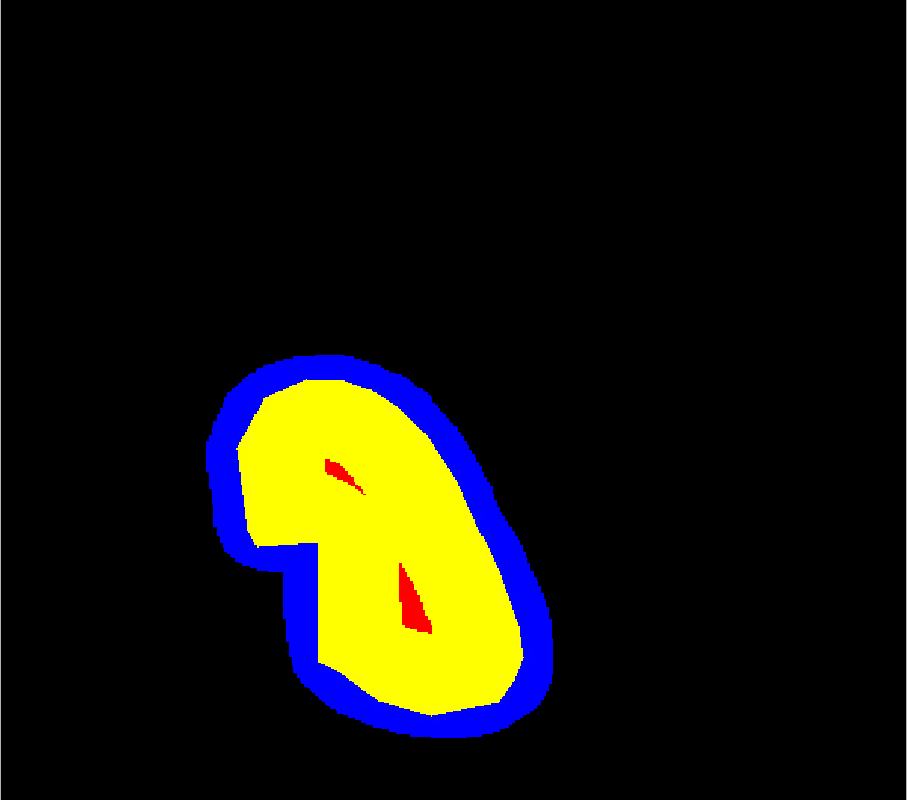
\includegraphics[width=0.24\textwidth]{../figures/learning/dist_crs_marginal90/754.png}
		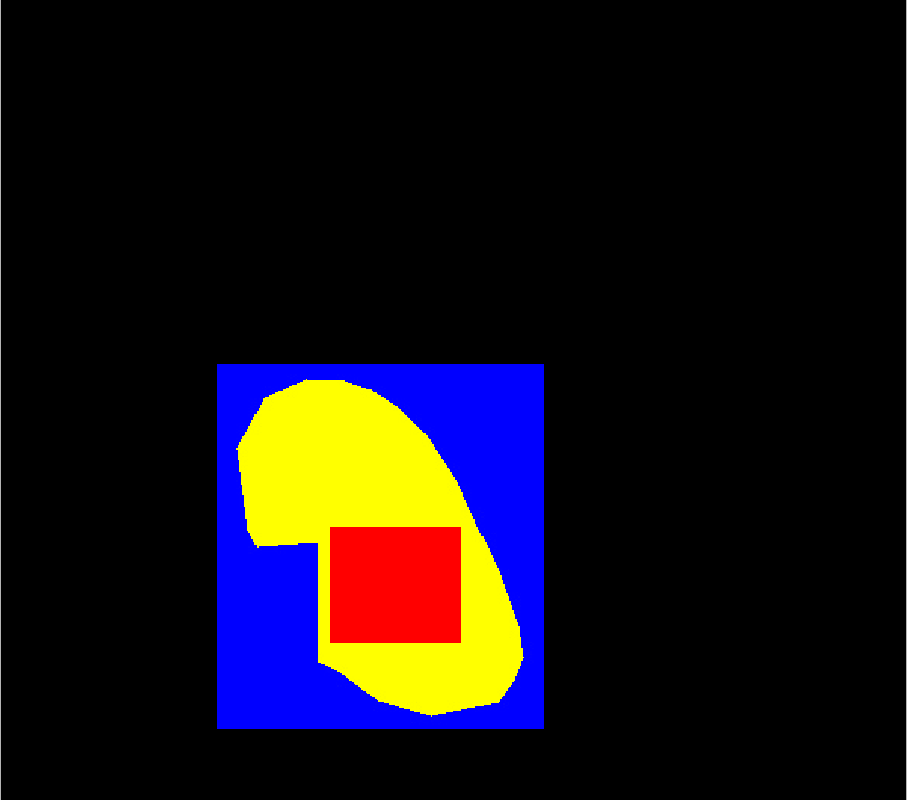
\includegraphics[width=0.24\textwidth]{../figures/learning/dist_bt_crs_marginal90/754.png}
	\end{center}
	\caption{Futher examples from the learning dataset. The layout of these figures is the same as for Figure \ref{fig:learning}.}
	\label{fig:learning3}
\end{figure}

\newpage
\subsubsection{Validition figures for the original and bounding box scores}\label{SS:furtherval}
\begin{figure}[h!]
	\begin{subfigure}{0.19\textwidth}
		\centering
		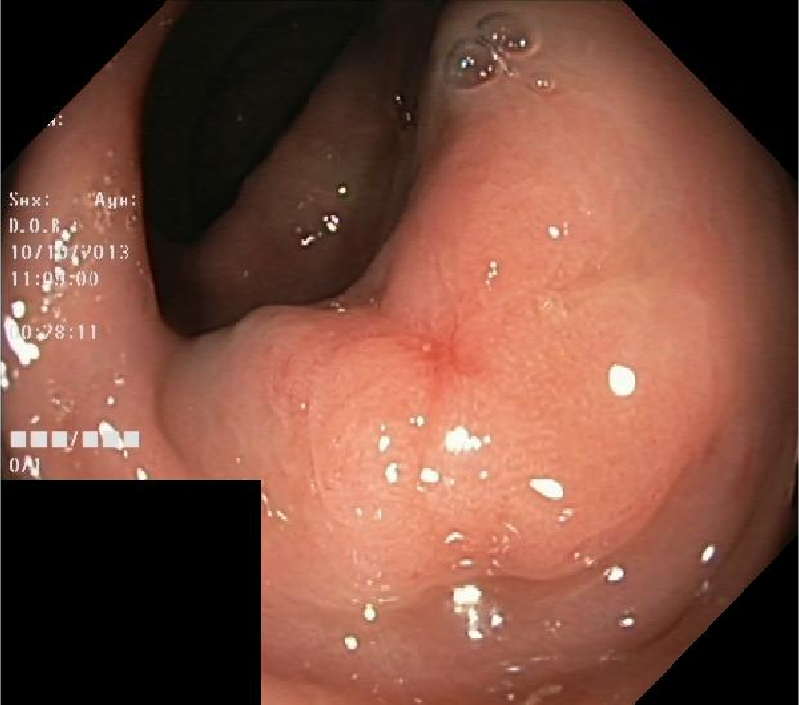
\includegraphics[width=\textwidth]{../figures/all_images/61.png}
		\label{fig:1}
	\end{subfigure}
	\begin{subfigure}{0.19\textwidth}
		\centering
		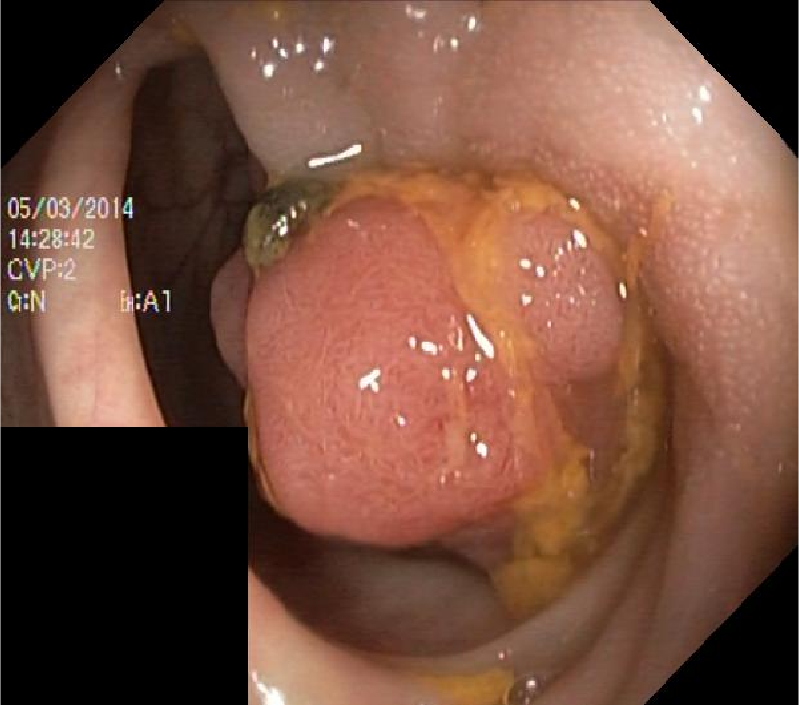
\includegraphics[width=\textwidth]{../figures/all_images/114.png}
		\label{fig:1}
	\end{subfigure}
	\begin{subfigure}{0.19\textwidth}
		\centering
		\includegraphics[width=\textwidth]{../figures/all_images/144.png}
		\label{fig:1}
	\end{subfigure}
	\begin{subfigure}{0.19\textwidth}
		\centering
		\includegraphics[width=\textwidth]{../figures/all_images/148.png}
		\label{fig:1}
	\end{subfigure}
	\begin{subfigure}{0.19\textwidth}
		\centering
		\includegraphics[width=\textwidth]{../figures/all_images/848.png}
		\label{fig:1}
	\end{subfigure}
	\vspace{-0.35cm}
	\\
	\begin{subfigure}{0.19\textwidth}
		\centering
		\includegraphics[width=\textwidth]{../figures/validation/val_crs_orig_90/61.png}
		\label{fig:1}
	\end{subfigure}
	\begin{subfigure}{0.19\textwidth}
		\centering
		\includegraphics[width=\textwidth]{../figures/validation/val_crs_orig_90/114.png}
		\label{fig:1}
	\end{subfigure}
	\begin{subfigure}{0.19\textwidth}
		\centering
		\includegraphics[width=\textwidth]{../figures/validation/val_crs_orig_90/144.png}
		\label{fig:1}
	\end{subfigure}
	\begin{subfigure}{0.19\textwidth}
		\centering
		\includegraphics[width=\textwidth]{../figures/validation/val_crs_orig_90/148.png}
		\label{fig:1}
	\end{subfigure}
	\begin{subfigure}{0.19\textwidth}
		\centering
		\includegraphics[width=\textwidth]{../figures/validation/val_crs_orig_90/848.png}
		\label{fig:1}
	\end{subfigure}
	\vspace{-0.35cm}
	\\
		\begin{subfigure}{0.19\textwidth}
		\centering
		\includegraphics[width=\textwidth]{../figures/validation/val_crs_bt_90/61.png}
		\label{fig:1}
	\end{subfigure}
	\begin{subfigure}{0.19\textwidth}
		\centering
		\includegraphics[width=\textwidth]{../figures/validation/val_crs_bt_90/114.png}
		\label{fig:1}
	\end{subfigure}
	\begin{subfigure}{0.19\textwidth}
		\centering
		\includegraphics[width=\textwidth]{../figures/validation/val_crs_bt_90/144.png}
		\label{fig:1}
	\end{subfigure}
	\begin{subfigure}{0.19\textwidth}
		\centering
		\includegraphics[width=\textwidth]{../figures/validation/val_crs_bt_90/148.png}
		\label{fig:1}
	\end{subfigure}
	\begin{subfigure}{0.19\textwidth}
		\centering
		\includegraphics[width=\textwidth]{../figures/validation/val_crs_bt_90/848.png}
		\label{fig:1}
	\end{subfigure}
	\vspace{-0.35cm}
	\\
	\begin{subfigure}{0.19\textwidth}
		\centering
		\includegraphics[width=\textwidth]{../figures/all_images/7.png}
		\label{fig:1}
	\end{subfigure}
	\begin{subfigure}{0.19\textwidth}
		\centering
		\includegraphics[width=\textwidth]{../figures/all_images/211.png}
		\label{fig:1}
	\end{subfigure}
	\begin{subfigure}{0.19\textwidth}
		\centering
		\includegraphics[width=\textwidth]{../figures/all_images/1062.png}
		\label{fig:1}
	\end{subfigure}
	\begin{subfigure}{0.19\textwidth}
		\centering
		\includegraphics[width=\textwidth]{../figures/all_images/398.png}
		\label{fig:1}
	\end{subfigure}
	\begin{subfigure}{0.19\textwidth}
		\centering
		\includegraphics[width=\textwidth]{../figures/all_images/269.png}
		\label{fig:1}
	\end{subfigure}
	\vspace{-0.35cm}
	\\
	\begin{subfigure}{0.19\textwidth}
		\centering
		\includegraphics[width=\textwidth]{../figures/validation/cal_crs_orig_90/7.png}
		\label{fig:1}
	\end{subfigure}
	\begin{subfigure}{0.19\textwidth}
		\centering
		\includegraphics[width=\textwidth]{../figures/validation/cal_crs_orig_90/211.png}
		\label{fig:1}
	\end{subfigure}
	\begin{subfigure}{0.19\textwidth}
		\centering
		\includegraphics[width=\textwidth]{../figures/validation/val_crs_orig_90/1062.png}
		\label{fig:1}
	\end{subfigure}
	\begin{subfigure}{0.19\textwidth}
		\centering
		\includegraphics[width=\textwidth]{../figures/validation/val_crs_orig_90/398.png}
		\label{fig:1}
	\end{subfigure}
	\begin{subfigure}{0.19\textwidth}
		\centering
		\includegraphics[width=\textwidth]{../figures/validation/cal_crs_orig_90/269.png}
		\label{fig:1}
	\end{subfigure}
	\vspace{-0.35cm}
	\\
	\begin{subfigure}{0.19\textwidth}
		\centering
		\includegraphics[width=\textwidth]{../figures/validation/cal_crs_bt_90/7.png}
		\label{fig:1}
	\end{subfigure}
	\begin{subfigure}{0.19\textwidth}
		\centering
		\includegraphics[width=\textwidth]{../figures/validation/cal_crs_bt_90/211.png}
		\label{fig:1}
	\end{subfigure}
	\begin{subfigure}{0.19\textwidth}
		\centering
		\includegraphics[width=\textwidth]{../figures/validation/val_crs_bt_90/1062.png}
		\label{fig:1}
	\end{subfigure}
	\begin{subfigure}{0.19\textwidth}
		\centering
		\includegraphics[width=\textwidth]{../figures/validation/val_crs_bt_90/398.png}
		\label{fig:1}
	\end{subfigure}
	\begin{subfigure}{0.19\textwidth}
		\centering
		\includegraphics[width=\textwidth]{../figures/validation/cal_crs_bt_90/269.png}
		\label{fig:1}
	\end{subfigure}
	\label{fig:grid}
	\caption{Conformal confidence sets for the polyps data examples from Figure \ref{fig:res} for alternative scores. In each set of panels the confidence obtained from using the original scores are shown in the middle row and those obtained from the bounding box scores are shown in the bottom row. As observed on the learning dataset the outer sets obtained when using the original scores are very large and uninformative.}\label{fig:polpysex}
\end{figure}
\newpage
\subsubsection{Additional validition figures}
\begin{figure}[h!]
	\begin{subfigure}{0.19\textwidth}
		\centering
		\includegraphics[width=\textwidth]{../figures/all_images/685.png}
		\label{fig:1}
	\end{subfigure}
	\begin{subfigure}{0.19\textwidth}
		\centering
		\includegraphics[width=\textwidth]{../figures/all_images/743.png}
		\label{fig:1}
	\end{subfigure}
	\begin{subfigure}{0.19\textwidth}
		\centering
		\includegraphics[width=\textwidth]{../figures/all_images/771.png}
		\label{fig:1}
	\end{subfigure}
	\begin{subfigure}{0.19\textwidth}
		\centering
		\includegraphics[width=\textwidth]{../figures/all_images/829.png}
		\label{fig:1}
	\end{subfigure}
	\begin{subfigure}{0.19\textwidth}
		\centering
		\includegraphics[width=\textwidth]{../figures/all_images/848.png}
		\label{fig:1}
	\end{subfigure}
	\vspace{-0.35cm}
	\\
	\begin{subfigure}{0.19\textwidth}
		\centering
		\includegraphics[width=\textwidth]{../figures/validation/val_crs_combo_90/685.png}
		\label{fig:1}
	\end{subfigure}
	\begin{subfigure}{0.19\textwidth}
		\centering
		\includegraphics[width=\textwidth]{../figures/validation/val_crs_combo_90/743.png}
		\label{fig:1}
	\end{subfigure}
	\begin{subfigure}{0.19\textwidth}
		\centering
		\includegraphics[width=\textwidth]{../figures/validation/val_crs_combo_90/771.png}
		\label{fig:1}
	\end{subfigure}
	\begin{subfigure}{0.19\textwidth}
		\centering
		\includegraphics[width=\textwidth]{../figures/validation/val_crs_combo_90/829.png}
		\label{fig:1}
	\end{subfigure}
	\begin{subfigure}{0.19\textwidth}
		\centering
		\includegraphics[width=\textwidth]{../figures/validation/val_crs_combo_90/848.png}
		\label{fig:1}
	\end{subfigure}
	\vspace{-0.35cm}
	\\
	\begin{subfigure}{0.19\textwidth}
		\centering
		\includegraphics[width=\textwidth]{../figures/validation/val_crs_orig_90/685.png}
		\label{fig:1}
	\end{subfigure}
	\begin{subfigure}{0.19\textwidth}
		\centering
		\includegraphics[width=\textwidth]{../figures/validation/val_crs_orig_90/743.png}
		\label{fig:1}
	\end{subfigure}
	\begin{subfigure}{0.19\textwidth}
		\centering
		\includegraphics[width=\textwidth]{../figures/validation/val_crs_orig_90/771.png}
		\label{fig:1}
	\end{subfigure}
	\begin{subfigure}{0.19\textwidth}
		\centering
		\includegraphics[width=\textwidth]{../figures/validation/val_crs_orig_90/829.png}
		\label{fig:1}
	\end{subfigure}
	\begin{subfigure}{0.19\textwidth}
		\centering
		\includegraphics[width=\textwidth]{../figures/validation/val_crs_orig_90/848.png}
		\label{fig:1}
	\end{subfigure}
		\vspace{-0.35cm}
	\\
	\begin{subfigure}{0.19\textwidth}
		\centering
		\includegraphics[width=\textwidth]{../figures/validation/val_crs_bt_90/685.png}
		\label{fig:1}
	\end{subfigure}
	\begin{subfigure}{0.19\textwidth}
		\centering
		\includegraphics[width=\textwidth]{../figures/validation/val_crs_bt_90/743.png}
		\label{fig:1}
	\end{subfigure}
	\begin{subfigure}{0.19\textwidth}
		\centering
		\includegraphics[width=\textwidth]{../figures/validation/val_crs_bt_90/771.png}
		\label{fig:1}
	\end{subfigure}
	\begin{subfigure}{0.19\textwidth}
		\centering
		\includegraphics[width=\textwidth]{../figures/validation/val_crs_bt_90/829.png}
		\label{fig:1}
	\end{subfigure}
	\begin{subfigure}{0.19\textwidth}
		\centering
		\includegraphics[width=\textwidth]{../figures/validation/val_crs_bt_90/848.png}
		\label{fig:1}
	\end{subfigure}
	\vspace{-0.35cm}
	\\
	\begin{subfigure}{0.19\textwidth}
		\centering
		\includegraphics[width=\textwidth]{../figures/all_images/50.png}
		\label{fig:1}
	\end{subfigure}
	\begin{subfigure}{0.19\textwidth}
		\centering
		\includegraphics[width=\textwidth]{../figures/all_images/138.png}
		\label{fig:1}
	\end{subfigure}
	\begin{subfigure}{0.19\textwidth}
		\centering
		\includegraphics[width=\textwidth]{../figures/all_images/179.png}
		\label{fig:1}
	\end{subfigure}
	\begin{subfigure}{0.19\textwidth}
		\centering
		\includegraphics[width=\textwidth]{../figures/all_images/483.png}
		\label{fig:1}
	\end{subfigure}
	\begin{subfigure}{0.19\textwidth}
		\centering
		\includegraphics[width=\textwidth]{../figures/all_images/1097.png}
		\label{fig:1}
	\end{subfigure}
	\vspace{-0.35cm}
	\\
	\begin{subfigure}{0.19\textwidth}
		\centering
		\includegraphics[width=\textwidth]{../figures/validation/val_crs_combo_90/50.png}
		\label{fig:1}
	\end{subfigure}
	\begin{subfigure}{0.19\textwidth}
		\centering
		\includegraphics[width=\textwidth]{../figures/validation/val_crs_combo_90/138.png}
		\label{fig:1}
	\end{subfigure}
	\begin{subfigure}{0.19\textwidth}
		\centering
		\includegraphics[width=\textwidth]{../figures/validation/val_crs_combo_90/179.png}
		\label{fig:1}
	\end{subfigure}
	\begin{subfigure}{0.19\textwidth}
		\centering
		\includegraphics[width=\textwidth]{../figures/validation/val_crs_combo_90/483.png}
		\label{fig:1}
	\end{subfigure}
	\begin{subfigure}{0.19\textwidth}
		\centering
		\includegraphics[width=\textwidth]{../figures/validation/val_crs_combo_90/1097.png}
		\label{fig:1}
	\end{subfigure}
		\vspace{-0.35cm}
	\\
	\begin{subfigure}{0.19\textwidth}
		\centering
		\includegraphics[width=\textwidth]{../figures/validation/val_crs_orig_90/50.png}
		\label{fig:1}
	\end{subfigure}
	\begin{subfigure}{0.19\textwidth}
		\centering
		\includegraphics[width=\textwidth]{../figures/validation/val_crs_orig_90/138.png}
		\label{fig:1}
	\end{subfigure}
	\begin{subfigure}{0.19\textwidth}
		\centering
		\includegraphics[width=\textwidth]{../figures/validation/val_crs_orig_90/179.png}
		\label{fig:1}
	\end{subfigure}
	\begin{subfigure}{0.19\textwidth}
		\centering
		\includegraphics[width=\textwidth]{../figures/validation/val_crs_orig_90/483.png}
		\label{fig:1}
	\end{subfigure}
	\begin{subfigure}{0.19\textwidth}
		\centering
		\includegraphics[width=\textwidth]{../figures/validation/val_crs_orig_90/1097.png}
		\label{fig:1}
	\end{subfigure}
			\vspace{-0.35cm}
	\\
	\begin{subfigure}{0.19\textwidth}
		\centering
		\includegraphics[width=\textwidth]{../figures/validation/val_crs_bt_90/50.png}
		\label{fig:1}
	\end{subfigure}
	\begin{subfigure}{0.19\textwidth}
		\centering
		\includegraphics[width=\textwidth]{../figures/validation/val_crs_bt_90/138.png}
		\label{fig:1}
	\end{subfigure}
	\begin{subfigure}{0.19\textwidth}
		\centering
		\includegraphics[width=\textwidth]{../figures/validation/val_crs_bt_90/179.png}
		\label{fig:1}
	\end{subfigure}
	\begin{subfigure}{0.19\textwidth}
		\centering
		\includegraphics[width=\textwidth]{../figures/validation/val_crs_bt_90/483.png}
		\label{fig:1}
	\end{subfigure}
	\begin{subfigure}{0.19\textwidth}
		\centering
		\includegraphics[width=\textwidth]{../figures/validation/val_crs_bt_90/1097.png}
		\label{fig:1}
	\end{subfigure}
	\label{fig:grid}
	\caption{Additional validition examples. In each example, after the original images, the rows are (from top to bottom) the combination of the original and distance transformed scores, then the original scores and finally the bounding box scores.}\label{fig:polpysex2}
\end{figure}

\newpage
\subsubsection{Confidence sets for the bounding boxes}
\begin{figure}[h!]
	\begin{subfigure}{0.19\textwidth}
		\centering
		\includegraphics[width=\textwidth]{../figures/all_images/61.png}
		\label{fig:1}
	\end{subfigure}
	\begin{subfigure}{0.19\textwidth}
		\centering
		\includegraphics[width=\textwidth]{../figures/all_images/114.png}
		\label{fig:1}
	\end{subfigure}
	\begin{subfigure}{0.19\textwidth}
		\centering
		\includegraphics[width=\textwidth]{../figures/all_images/144.png}
		\label{fig:1}
	\end{subfigure}
	\begin{subfigure}{0.19\textwidth}
		\centering
		\includegraphics[width=\textwidth]{../figures/all_images/148.png}
		\label{fig:1}
	\end{subfigure}
	\begin{subfigure}{0.19\textwidth}
		\centering
		\includegraphics[width=\textwidth]{../figures/all_images/251.png}
		\label{fig:1}
	\end{subfigure}
	\vspace{-0.35cm}
	\\
	\begin{subfigure}{0.19\textwidth}
		\centering
		\includegraphics[width=\textwidth]{../figures/validation/boundary_box_90/61.png}
		\label{fig:1}
	\end{subfigure}
	\begin{subfigure}{0.19\textwidth}
		\centering
		\includegraphics[width=\textwidth]{../figures/validation/boundary_box_90/114.png}
		\label{fig:1}
	\end{subfigure}
	\begin{subfigure}{0.19\textwidth}
		\centering
		\includegraphics[width=\textwidth]{../figures/validation/boundary_box_90/144.png}
		\label{fig:1}
	\end{subfigure}
	\begin{subfigure}{0.19\textwidth}
		\centering
		\includegraphics[width=\textwidth]{../figures/validation/boundary_box_90/148.png}
		\label{fig:1}
	\end{subfigure}
	\begin{subfigure}{0.19\textwidth}
		\centering
		\includegraphics[width=\textwidth]{../figures/validation/boundary_box_90/251.png}
		\label{fig:1}
	\end{subfigure}
	\vspace{-0.35cm}
	\\
	\begin{subfigure}{0.19\textwidth}
		\centering
		\includegraphics[width=\textwidth]{../figures/all_images/7.png}
		\label{fig:1}
	\end{subfigure}
	\begin{subfigure}{0.19\textwidth}
		\centering
		\includegraphics[width=\textwidth]{../figures/all_images/211.png}
		\label{fig:1}
	\end{subfigure}
	\begin{subfigure}{0.19\textwidth}
		\centering
		\includegraphics[width=\textwidth]{../figures/all_images/1062.png}
		\label{fig:1}
	\end{subfigure}
	\begin{subfigure}{0.19\textwidth}
		\centering
		\includegraphics[width=\textwidth]{../figures/all_images/398.png}
		\label{fig:1}
	\end{subfigure}
	\begin{subfigure}{0.19\textwidth}
		\centering
		\includegraphics[width=\textwidth]{../figures/all_images/269.png}
		\label{fig:1}
	\end{subfigure}
	\vspace{-0.35cm}
	\\
	\begin{subfigure}{0.19\textwidth}
		\centering
		\includegraphics[width=\textwidth]{../figures/validation/boundary_box_90/7.png}
		\label{fig:1}
	\end{subfigure}
	\begin{subfigure}{0.19\textwidth}
		\centering
		\includegraphics[width=\textwidth]{../figures/validation/boundary_box_90/211.png}
		\label{fig:1}
	\end{subfigure}
	\begin{subfigure}{0.19\textwidth}
		\centering
		\includegraphics[width=\textwidth]{../figures/validation/boundary_box_90/1062.png}
		\label{fig:1}
	\end{subfigure}
	\begin{subfigure}{0.19\textwidth}
		\centering
		\includegraphics[width=\textwidth]{../figures/validation/boundary_box_90/398.png}
		\label{fig:1}
	\end{subfigure}
	\begin{subfigure}{0.19\textwidth}
		\centering
		\includegraphics[width=\textwidth]{../figures/validation/boundary_box_90/269.png}
		\label{fig:1}
	\end{subfigure}
	\label{fig:grid}
	\caption{Conformal confidence sets for the boundary boxes themselves using the approach introduced in Section \ref{AA:BBtheory}. The ground truth outer bounding boxes are shown in yellow.}\label{fig:resbb}
\end{figure}

\subsubsection{Joint 90\% confidence regions}
\begin{figure}[h!]
	\begin{subfigure}{0.19\textwidth}
		\centering
		\includegraphics[width=\textwidth]{../figures/validation/joint_90/61.png}
		\label{fig:1}
	\end{subfigure}
	\begin{subfigure}{0.19\textwidth}
		\centering
		\includegraphics[width=\textwidth]{../figures/validation/joint_90/114.png}
		\label{fig:1}
	\end{subfigure}
	\begin{subfigure}{0.19\textwidth}
		\centering
		\includegraphics[width=\textwidth]{../figures/validation/joint_90/144.png}
		\label{fig:1}
	\end{subfigure}
	\begin{subfigure}{0.19\textwidth}
		\centering
		\includegraphics[width=\textwidth]{../figures/validation/joint_90/148.png}
		\label{fig:1}
	\end{subfigure}
	\begin{subfigure}{0.19\textwidth}
		\centering
		\includegraphics[width=\textwidth]{../figures/validation/joint_90/251.png}
		\label{fig:1}
	\end{subfigure}
	\vspace{-0.35cm}
	\\
	\begin{subfigure}{0.19\textwidth}
		\centering
		\includegraphics[width=\textwidth]{../figures/validation/joint_90/7.png}
		\label{fig:1}
	\end{subfigure}
	\begin{subfigure}{0.19\textwidth}
		\centering
		\includegraphics[width=\textwidth]{../figures/validation/joint_90/211.png}
		\label{fig:1}
	\end{subfigure}
	\begin{subfigure}{0.19\textwidth}
		\centering
		\includegraphics[width=\textwidth]{../figures/validation/joint_90/1062.png}
		\label{fig:1}
	\end{subfigure}
	\begin{subfigure}{0.19\textwidth}
		\centering
		\includegraphics[width=\textwidth]{../figures/validation/joint_90/398.png}
		\label{fig:1}
	\end{subfigure}
	\begin{subfigure}{0.19\textwidth}
		\centering
		\includegraphics[width=\textwidth]{../figures/validation/joint_90/269.png}
		\label{fig:1}
	\end{subfigure}
	\label{fig:grid}
	\caption{Joint 90\% conformal confidence sets obtained using Corollary \ref{cor:weighting}, with $\alpha_1 = 0.02$ and $\alpha_2 = 0.08$, for the polyps images in Figure \ref{fig:res}.}\label{fig:joint}
\end{figure}
\newpage
\subsubsection{Marginal 80 \% Confidence regions}
\begin{figure}[h!]
	\begin{subfigure}{0.19\textwidth}
		\centering
		\includegraphics[width=\textwidth]{../figures/validation/val_crs_combo_80/61.png}
		\label{fig:1}
	\end{subfigure}
	\begin{subfigure}{0.19\textwidth}
		\centering
		\includegraphics[width=\textwidth]{../figures/validation/val_crs_combo_80/114.png}
		\label{fig:1}
	\end{subfigure}
	\begin{subfigure}{0.19\textwidth}
		\centering
		\includegraphics[width=\textwidth]{../figures/validation/val_crs_combo_80/144.png}
		\label{fig:1}
	\end{subfigure}
	\begin{subfigure}{0.19\textwidth}
		\centering
		\includegraphics[width=\textwidth]{../figures/validation/val_crs_combo_80/148.png}
		\label{fig:1}
	\end{subfigure}
	\begin{subfigure}{0.19\textwidth}
		\centering
		\includegraphics[width=\textwidth]{../figures/validation/val_crs_combo_80/251.png}
		\label{fig:1}
	\end{subfigure}
	\vspace{-0.35cm}
	\\
	\begin{subfigure}{0.19\textwidth}
		\centering
		\includegraphics[width=\textwidth]{../figures/validation/val_crs_combo_80/7.png}
		\label{fig:1}
	\end{subfigure}
	\begin{subfigure}{0.19\textwidth}
		\centering
		\includegraphics[width=\textwidth]{../figures/validation/val_crs_combo_80/211.png}
		\label{fig:1}
	\end{subfigure}
	\begin{subfigure}{0.19\textwidth}
		\centering
		\includegraphics[width=\textwidth]{../figures/validation/val_crs_combo_80/1062.png}
		\label{fig:1}
	\end{subfigure}
	\begin{subfigure}{0.19\textwidth}
		\centering
		\includegraphics[width=\textwidth]{../figures/validation/val_crs_combo_80/398.png}
		\label{fig:1}
	\end{subfigure}
	\begin{subfigure}{0.19\textwidth}
		\centering
		\includegraphics[width=\textwidth]{../figures/validation/val_crs_combo_80/269.png}
		\label{fig:1}
	\end{subfigure}
	\label{fig:grid}
	\caption{Marginal 80\% conformal confidence sets obtained for the polyps images in Figure \ref{fig:res}.}\label{fig:joint2}
\end{figure}
\subsubsection{Marginal 95 \% Confidence regions}

\begin{figure}[h!]
	\begin{subfigure}{0.19\textwidth}
		\centering
		\includegraphics[width=\textwidth]{../figures/validation/val_crs_combo_95/61.png}
		\label{fig:1}
	\end{subfigure}
	\begin{subfigure}{0.19\textwidth}
		\centering
		\includegraphics[width=\textwidth]{../figures/validation/val_crs_combo_95/114.png}
		\label{fig:1}
	\end{subfigure}
	\begin{subfigure}{0.19\textwidth}
		\centering
		\includegraphics[width=\textwidth]{../figures/validation/val_crs_combo_95/144.png}
		\label{fig:1}
	\end{subfigure}
	\begin{subfigure}{0.19\textwidth}
		\centering
		\includegraphics[width=\textwidth]{../figures/validation/val_crs_combo_95/148.png}
		\label{fig:1}
	\end{subfigure}
	\begin{subfigure}{0.19\textwidth}
		\centering
		\includegraphics[width=\textwidth]{../figures/validation/val_crs_combo_95/251.png}
		\label{fig:1}
	\end{subfigure}
	\vspace{-0.35cm}
	\\
	\begin{subfigure}{0.19\textwidth}
		\centering
		\includegraphics[width=\textwidth]{../figures/validation/val_crs_combo_95/7.png}
		\label{fig:1}
	\end{subfigure}
	\begin{subfigure}{0.19\textwidth}
		\centering
		\includegraphics[width=\textwidth]{../figures/validation/val_crs_combo_95/211.png}
		\label{fig:1}
	\end{subfigure}
	\begin{subfigure}{0.19\textwidth}
		\centering
		\includegraphics[width=\textwidth]{../figures/validation/val_crs_combo_95/1062.png}
		\label{fig:1}
	\end{subfigure}
	\begin{subfigure}{0.19\textwidth}
		\centering
		\includegraphics[width=\textwidth]{../figures/validation/joint_90/398.png}
		\label{fig:1}
	\end{subfigure}
	\begin{subfigure}{0.19\textwidth}
		\centering
		\includegraphics[width=\textwidth]{../figures/validation/joint_90/269.png}
		\label{fig:1}
	\end{subfigure}
	\label{fig:grid}
	\caption{Marginal 95\% conformal confidence sets obtained using for the polyps images in Figure \ref{fig:res}. These sets are also joint 90\% confidence sets with equally weighted $\alpha_1 = \alpha_2 = 0.05$. The influence of the weighting scheme can therefore examined by comparing to Figure \ref{fig:joint}.}\label{fig:joint3}
\end{figure}
\newpage
\subsubsection{Histograms of the coverage}
\begin{figure}[h!]
	\begin{center}
		\includegraphics[width=0.32\textwidth]{../figures/validation/val_hist_orig_inner.pdf}
		\includegraphics[width=0.32\textwidth]{../figures/validation/val_hist_dt_inner.pdf}
		\includegraphics[width=0.32\textwidth]{../figures/validation/val_hist_bt_inner.pdf}\\
		\includegraphics[width=0.32\textwidth]{../figures/validation/val_hist_orig_outer.pdf}
		\includegraphics[width=0.32\textwidth]{../figures/validation/val_hist_dt_outer.pdf}
		\includegraphics[width=0.32\textwidth]{../figures/validation/val_hist_bt_outer.pdf}
	\end{center}
	\caption{Histograms of the coverage rates obtained across each of the validation resamples for 90\% inner and outer marginal confidence sets. We plot the results for the original scores, distance transformed scores (DT) and boundary box scores (BB) from left to right. The bounding box scores are discontinuous which is the cause of the discreteness of the rightmost histograms.}\label{fig:valhist}
\end{figure}

\subsubsection{Comparing the proportion}

\begin{figure}[h!]
	\begin{center}
		\includegraphics[width=0.46\textwidth]{../figures/efficiency/inner_proportion.pdf}
		\quad\quad
		\includegraphics[width=0.45\textwidth]{../figures/efficiency/outer_proportion.pdf}
	\end{center}
	\caption{Measuring the proportion of the entire image which is under/over covered by the respective confidence sets. Left: proportion of the image which lies within the true mask but outside of the inner set. Right: proportion of the image which lies within the confidence set but outside of the true mask. For both a lower proportion corresponds to increased precision. }\label{fig:efficiency2}
\end{figure}

\newpage
\subsection{Additional settings for brain mask segmentation}

\subsubsection{Comparing original and distance transformed scores on the learning dataset}\label{brainlearn}
\begin{figure}[h!] % 'r' for right, and setting the width
	%	\captionsetup{width=0.58\textwidth}
	\centering
	% First row of images
	\begin{subfigure}{0.16\textwidth}
		\centering
		\includegraphics[width=\textwidth]{../figures/brain_seg/learning/orig_images/1_orig.png}
		\label{fig:1}
	\end{subfigure}
	\begin{subfigure}{0.16\textwidth}
		\centering
		\includegraphics[width=\textwidth]{../figures/brain_seg/learning/orig_images/2_orig.png}
		\label{fig:2}
	\end{subfigure}
	\begin{subfigure}{0.16\textwidth}
		\centering
		\includegraphics[width=\textwidth]{../figures/brain_seg/learning/orig_images/3_orig.png}
		\label{fig:3}
	\end{subfigure}
	\begin{subfigure}{0.16\textwidth}
		\centering
		\includegraphics[width=\textwidth]{../figures/brain_seg/learning/orig_images/4_orig.png}
		\label{fig:4}
	\end{subfigure}
	\begin{subfigure}{0.16\textwidth}
		\centering
		\includegraphics[width=\textwidth]{../figures/brain_seg/learning/orig_images/5_orig.png}
		\label{fig:5}
	\end{subfigure}
	%		
	% Small vertical space adjustmen
	\\
	\vspace{-0.35cm}
	% Second row of images
	\begin{subfigure}{0.16\textwidth}
		\centering
		\includegraphics[width=\textwidth]{../figures/brain_seg/learning/dt_scores/1_crs.png}
		\label{fig:6}
	\end{subfigure}
	\begin{subfigure}{0.16\textwidth}
		\centering
		\includegraphics[width=\textwidth]{../figures/brain_seg/learning/dt_scores/2_crs.png}
		\label{fig:7}
	\end{subfigure}
	\begin{subfigure}{0.16\textwidth}
		\centering
		\includegraphics[width=\textwidth]{../figures/brain_seg/learning/dt_scores/3_crs.png}
		\label{fig:8}
	\end{subfigure}
	\begin{subfigure}{0.16\textwidth}
		\centering
		\includegraphics[width=\textwidth]{../figures/brain_seg/learning/dt_scores/4_crs.png}
		\label{fig:9}
	\end{subfigure}
	\begin{subfigure}{0.16\textwidth}
		\centering
		\includegraphics[width=\textwidth]{../figures/brain_seg/learning/dt_scores/5_crs.png}
		\label{fig:10}
	\end{subfigure}
	\\
	\vspace{-0.35cm}
	% Second row of images
	\begin{subfigure}{0.16\textwidth}
		\centering
		\includegraphics[width=\textwidth]{../figures/brain_seg/learning/orig_scores/1_origcrs.png}
		\label{fig:6}
	\end{subfigure}
	\begin{subfigure}{0.16\textwidth}
		\centering
		\includegraphics[width=\textwidth]{../figures/brain_seg/learning/orig_scores/2_origcrs.png}
		\label{fig:7}
	\end{subfigure}
	\begin{subfigure}{0.16\textwidth}
		\centering
		\includegraphics[width=\textwidth]{../figures/brain_seg/learning/orig_scores/3_origcrs.png}
		\label{fig:8}
	\end{subfigure}
	\begin{subfigure}{0.16\textwidth}
		\centering
		\includegraphics[width=\textwidth]{../figures/brain_seg/learning/orig_scores/4_origcrs.png}
		\label{fig:9}
	\end{subfigure}
	\begin{subfigure}{0.16\textwidth}
		\centering
		\includegraphics[width=\textwidth]{../figures/brain_seg/learning/orig_scores/5_origcrs.png}
		\label{fig:10}
	\end{subfigure}
	% Caption for the figure
	\caption{\nt{Learning the best transformation for brain mask segmentation. First row: original images from different subjects. Second row: confidence sets provided by calibrating the distance transformed scores on the learning dataset. Third row: confidence sets produced using the original scores on the learning dataset. Using the original scores produced very bad results. Instead the distance transformation is a big improvement. Note that the improvement obtained by using the distance scores is even more when using the full calibration data, see Figure \ref{fig:brain}. This is because the learning dataset is relatively small and does not capture the full picture. The results at test time for the original scores are equally bad as for the learning data, see Figure \ref{fig:brain2}.}}
	\label{fig:brain3}
\end{figure}

\newpage
\subsubsection{Comparing smooth transformed scores on the learning dataset}\label{brainsmooth}

\begin{figure}[h!] % 'r' for right, and setting the width
	%	\captionsetup{width=0.58\textwidth}
	\centering
	% First row of images
	\begin{subfigure}{0.16\textwidth}
		\centering
		\includegraphics[width=\textwidth]{../figures/brain_seg/learning/orig_images/1_orig.png}
		\label{fig:1}
	\end{subfigure}
	\begin{subfigure}{0.16\textwidth}
		\centering
		\includegraphics[width=\textwidth]{../figures/brain_seg/learning/orig_images/2_orig.png}
		\label{fig:2}
	\end{subfigure}
	\begin{subfigure}{0.16\textwidth}
		\centering
		\includegraphics[width=\textwidth]{../figures/brain_seg/learning/orig_images/3_orig.png}
		\label{fig:3}
	\end{subfigure}
	\begin{subfigure}{0.16\textwidth}
		\centering
		\includegraphics[width=\textwidth]{../figures/brain_seg/learning/orig_images/4_orig.png}
		\label{fig:4}
	\end{subfigure}
	\begin{subfigure}{0.16\textwidth}
		\centering
		\includegraphics[width=\textwidth]{../figures/brain_seg/learning/orig_images/5_orig.png}
		\label{fig:5}
	\end{subfigure}
	%		
	% Small vertical space adjustmen
	\\
	\vspace{-0.35cm}
	% Second row of images
	\begin{subfigure}{0.16\textwidth}
		\centering
		\includegraphics[width=\textwidth]{../figures/brain_seg/learning/smooth_scores/1_FWHM_15.png}
		\label{fig:6}
	\end{subfigure}
	\begin{subfigure}{0.16\textwidth}
		\centering
		\includegraphics[width=\textwidth]{../figures/brain_seg/learning/smooth_scores/2_FWHM_15.png}
		\label{fig:7}
	\end{subfigure}
	\begin{subfigure}{0.16\textwidth}
		\centering
		\includegraphics[width=\textwidth]{../figures/brain_seg/learning/smooth_scores/3_FWHM_15.png}
		\label{fig:8}
	\end{subfigure}
	\begin{subfigure}{0.16\textwidth}
		\centering
		\includegraphics[width=\textwidth]{../figures/brain_seg/learning/smooth_scores/4_FWHM_15.png}
		\label{fig:9}
	\end{subfigure}
	\begin{subfigure}{0.16\textwidth}
		\centering
		\includegraphics[width=\textwidth]{../figures/brain_seg/learning/smooth_scores/5_FWHM_15.png}
		\label{fig:10}
	\end{subfigure}
	\\
	\vspace{-0.35cm}
	% Second row of images
	\begin{subfigure}{0.16\textwidth}
		\centering
		\includegraphics[width=\textwidth]{../figures/brain_seg/learning/smooth_scores/1_FWHM_10.png}
		\label{fig:6}
	\end{subfigure}
	\begin{subfigure}{0.16\textwidth}
		\centering
		\includegraphics[width=\textwidth]{../figures/brain_seg/learning/smooth_scores/2_FWHM_10.png}
		\label{fig:7}
	\end{subfigure}
	\begin{subfigure}{0.16\textwidth}
		\centering
		\includegraphics[width=\textwidth]{../figures/brain_seg/learning/smooth_scores/3_FWHM_10.png}
		\label{fig:8}
	\end{subfigure}
	\begin{subfigure}{0.16\textwidth}
		\centering
		\includegraphics[width=\textwidth]{../figures/brain_seg/learning/smooth_scores/4_FWHM_10.png}
		\label{fig:9}
	\end{subfigure}
	\begin{subfigure}{0.16\textwidth}
		\centering
		\includegraphics[width=\textwidth]{../figures/brain_seg/learning/smooth_scores/5_FWHM_10.png}
		\label{fig:10}
	\end{subfigure}
		\\
	\vspace{-0.35cm}
	% Second row of images
	\begin{subfigure}{0.16\textwidth}
		\centering
		\includegraphics[width=\textwidth]{../figures/brain_seg/learning/smooth_scores/1_FWHM_15.png}
		\label{fig:6}
	\end{subfigure}
	\begin{subfigure}{0.16\textwidth}
		\centering
		\includegraphics[width=\textwidth]{../figures/brain_seg/learning/smooth_scores/2_FWHM_15.png}
		\label{fig:7}
	\end{subfigure}
	\begin{subfigure}{0.16\textwidth}
		\centering
		\includegraphics[width=\textwidth]{../figures/brain_seg/learning/smooth_scores/3_FWHM_15.png}
		\label{fig:8}
	\end{subfigure}
	\begin{subfigure}{0.16\textwidth}
		\centering
		\includegraphics[width=\textwidth]{../figures/brain_seg/learning/smooth_scores/4_FWHM_15.png}
		\label{fig:9}
	\end{subfigure}
	\begin{subfigure}{0.16\textwidth}
		\centering
		\includegraphics[width=\textwidth]{../figures/brain_seg/learning/smooth_scores/5_FWHM_15.png}
		\label{fig:10}
	\end{subfigure}
	\\
	\vspace{-0.35cm}
	% Second row of images
	\begin{subfigure}{0.16\textwidth}
		\centering
		\includegraphics[width=\textwidth]{../figures/brain_seg/learning/smooth_scores/1_FWHM_20.png}
		\label{fig:6}
	\end{subfigure}
	\begin{subfigure}{0.16\textwidth}
		\centering
		\includegraphics[width=\textwidth]{../figures/brain_seg/learning/smooth_scores/2_FWHM_20.png}
		\label{fig:7}
	\end{subfigure}
	\begin{subfigure}{0.16\textwidth}
		\centering
		\includegraphics[width=\textwidth]{../figures/brain_seg/learning/smooth_scores/3_FWHM_20.png}
		\label{fig:8}
	\end{subfigure}
	\begin{subfigure}{0.16\textwidth}
		\centering
		\includegraphics[width=\textwidth]{../figures/brain_seg/learning/smooth_scores/4_FWHM_20.png}
		\label{fig:9}
	\end{subfigure}
	\begin{subfigure}{0.16\textwidth}
		\centering
		\includegraphics[width=\textwidth]{../figures/brain_seg/learning/smooth_scores/5_FWHM_20.png}
		\label{fig:10}
	\end{subfigure}
		\\
	\vspace{-0.35cm}
	% Second row of images
	\begin{subfigure}{0.16\textwidth}
		\centering
		\includegraphics[width=\textwidth]{../figures/brain_seg/learning/smooth_scores/1_FWHM_20.png}
		\label{fig:6}
	\end{subfigure}
	\begin{subfigure}{0.16\textwidth}
		\centering
		\includegraphics[width=\textwidth]{../figures/brain_seg/learning/smooth_scores/2_FWHM_20.png}
		\label{fig:7}
	\end{subfigure}
	\begin{subfigure}{0.16\textwidth}
		\centering
		\includegraphics[width=\textwidth]{../figures/brain_seg/learning/smooth_scores/3_FWHM_20.png}
		\label{fig:8}
	\end{subfigure}
	\begin{subfigure}{0.16\textwidth}
		\centering
		\includegraphics[width=\textwidth]{../figures/brain_seg/learning/smooth_scores/4_FWHM_20.png}
		\label{fig:9}
	\end{subfigure}
	\begin{subfigure}{0.16\textwidth}
		\centering
		\includegraphics[width=\textwidth]{../figures/brain_seg/learning/smooth_scores/5_FWHM_20.png}
		\label{fig:10}
	\end{subfigure}
	% Caption for the figure
	\caption{\nt{Inner and outer sets computed by comparing smooth score transformations on the learning dataset. Scores were smoothed using a Gaussian kernel with full width at half maximum (FWHM) taking values in $\lbrace 5,10,15,20,25\rbrace$ mm. The resulting inner and outer sets based on increasing levels of applied smoothness are shown from top to bottom. The performance appears to peak at 20mm. }}
	\label{fig:brain3}
\end{figure}
\newpage
\subsubsection{Comparing original and distance transformed scores on the test dataset}\label{braintest}
	\begin{figure}[h!] % 'r' for right, and setting the width
%	\captionsetup{width=0.58\textwidth}
	\centering
	% First row of images
	\begin{subfigure}{0.16\textwidth}
		\centering
		\includegraphics[width=\textwidth]{../figures/brain_seg/test/orig_images/101_orig.png}
		\label{fig:1}
	\end{subfigure}
	\begin{subfigure}{0.16\textwidth}
		\centering
		\includegraphics[width=\textwidth]{../figures/brain_seg/test/orig_images/107_orig.png}
		\label{fig:2}
	\end{subfigure}
	\begin{subfigure}{0.16\textwidth}
		\centering
		\includegraphics[width=\textwidth]{../figures/brain_seg/test/orig_images/106_orig.png}
		\label{fig:3}
	\end{subfigure}
	\begin{subfigure}{0.16\textwidth}
		\centering
		\includegraphics[width=\textwidth]{../figures/brain_seg/test/orig_images/111_orig.png}
		\label{fig:4}
	\end{subfigure}
			\begin{subfigure}{0.16\textwidth}
					\centering
					\includegraphics[width=\textwidth]{../figures/brain_seg/test/orig_images/120_orig.png}
					\label{fig:5}
				\end{subfigure}
	%		
	% Small vertical space adjustmen
		\\
	\vspace{-0.35cm}
	% Second row of images
	\begin{subfigure}{0.16\textwidth}
		\centering
		\includegraphics[width=\textwidth]{../figures/brain_seg/test/dt_scores/101_crs.png}
		\label{fig:6}
	\end{subfigure}
	\begin{subfigure}{0.16\textwidth}
		\centering
		\includegraphics[width=\textwidth]{../figures/brain_seg/test/dt_scores/107_crs.png}
		\label{fig:7}
	\end{subfigure}
	\begin{subfigure}{0.16\textwidth}
		\centering
		\includegraphics[width=\textwidth]{../figures/brain_seg/test/dt_scores/106_crs.png}
		\label{fig:8}
	\end{subfigure}
	\begin{subfigure}{0.16\textwidth}
		\centering
		\includegraphics[width=\textwidth]{../figures/brain_seg/test/dt_scores/111_crs.png}
		\label{fig:9}
	\end{subfigure}
			\begin{subfigure}{0.16\textwidth}
					\centering
					\includegraphics[width=\textwidth]{../figures/brain_seg/test/dt_scores/120_crs.png}
					\label{fig:10}
				\end{subfigure}
		\\
	\vspace{-0.35cm}
	% Second row of images
	\begin{subfigure}{0.16\textwidth}
		\centering
		\includegraphics[width=\textwidth]{../figures/brain_seg/test/orig_scores/101_origcrs.png}
		\label{fig:6}
	\end{subfigure}
	\begin{subfigure}{0.16\textwidth}
		\centering
		\includegraphics[width=\textwidth]{../figures/brain_seg/test/orig_scores/107_origcrs.png}
		\label{fig:7}
	\end{subfigure}
	\begin{subfigure}{0.16\textwidth}
		\centering
		\includegraphics[width=\textwidth]{../figures/brain_seg/test/orig_scores/106_origcrs.png}
		\label{fig:8}
	\end{subfigure}
	\begin{subfigure}{0.16\textwidth}
		\centering
		\includegraphics[width=\textwidth]{../figures/brain_seg/test/orig_scores/111_origcrs.png}
		\label{fig:9}
	\end{subfigure}
	\begin{subfigure}{0.16\textwidth}
		\centering
		\includegraphics[width=\textwidth]{../figures/brain_seg/test/orig_scores/120_origcrs.png}
		\label{fig:10}
	\end{subfigure}
			\\
	\vspace{-0.35cm}
	% Second row of images
	\begin{subfigure}{0.16\textwidth}
		\centering
		\includegraphics[width=\textwidth]{../figures/brain_seg/test/smooth_scores/101_FWHM_20.png}
		\label{fig:6}
	\end{subfigure}
	\begin{subfigure}{0.16\textwidth}
		\centering
		\includegraphics[width=\textwidth]{../figures/brain_seg/test/smooth_scores/107_FWHM_20.png}
		\label{fig:7}
	\end{subfigure}
	\begin{subfigure}{0.16\textwidth}
		\centering
		\includegraphics[width=\textwidth]{../figures/brain_seg/test/smooth_scores/106_FWHM_20.png}
		\label{fig:8}
	\end{subfigure}
	\begin{subfigure}{0.16\textwidth}
		\centering
		\includegraphics[width=\textwidth]{../figures/brain_seg/test/smooth_scores/111_FWHM_20.png}
		\label{fig:9}
	\end{subfigure}
	\begin{subfigure}{0.16\textwidth}
		\centering
		\includegraphics[width=\textwidth]{../figures/brain_seg/test/smooth_scores/120_FWHM_20.png}
		\label{fig:10}
	\end{subfigure}
	\vspace{-0.5cm}
	% Caption for the figure
	\caption{\nt{Inner and outer confidence sets for brain mask segmentation using the distance transformed and original scores. Top row: brain images for each subject. 2nd row: the inner and outer confidence sets produced by calibrating the distance transformed scores on the calibration dataset. 3rd row:  the inner and outer confidence sets produced by calibrating the original scores on the calibration dataset. 4th row:  the inner and outer confidence sets produced by calibrating the smoothed scores (smoothed with an isotropic Guassian kernel of 20mm - chosen because it performed the best on the learning dataset). As for the learning dataset the original scores perform very poorly and are not able to separate the background from the segmented masks with confidence. Instead the distance transformed scores do a very good job at segmenting the mask. Indeed they do slightly better on the calibrated dataset than on the learning dataset. The smooth scores improve on the original scores but do not provide as tight bounds as the distance transformed scores for neither inner nor outer sets.}}
	\label{fig:brain2}
\end{figure}

\newpage
\subsubsection{Computing the coverage for the brain imaging data}\label{SS:val2}
In order to study the coverage rate of the methods in the context of the brain imaging application we peform a similar validation to that described in Section \ref{SS:cov} for polyps segmentation. To do so we divide the 474 subjects left, after excluding the learning dataset, into 300 calibration and 174 test images. We do this 1000 times, randomly sampling the sets of 300 and 174 images respectively and measuring the coverage in each run. We average the coverage over the 1000 runs and display the results in Figure \ref{fig:coverage2}. Note that unlike the box scores considered in Section \ref{SS:cov}, the smooth scores are not discrete so do not display discreteness issues at lower levels of coverage. 
\begin{figure}[h!]
	\begin{center}
		\includegraphics[width=0.4\textwidth]{../figures/coverage/inner_coverage_1.pdf}
		%		\quad\quad
		\includegraphics[width=0.4\textwidth]{../figures/coverage/outer_coverage_1.pdf}
		%		\includegraphics[width=0.24\textwidth]{../figures/efficiency/inner_ratio.pdf}
		%		%		\quad\quad
		%		%		\hspace{-0.8cm}
		%		\includegraphics[width=0.24\textwidth]{../figures/efficiency/outer_ratio.pdf}
	\end{center}
	\caption{Coverage levels of the inner and outer sets averaged over 1000 validations for the original, distance transformed (DT) and smoothed scores (smoothed with a full width at half maximum of 20mm). The nominal rate is acheived in all settings considered.}\label{fig:coverage2}
\end{figure}

\newpage
\subsection{Additional settings for teeth segmentation}\label{A:teeth}

\subsubsection{Comparing original and distance transformed scores on the learning dataset}\label{teethlearnorig}

\begin{figure}[h!]
	\begin{subfigure}{0.16\textwidth}
		\centering
		\includegraphics[width=\textwidth]{../figures/teeth/learning/orig_images/1_orig.png}
		\label{fig:1}
	\end{subfigure}
	\begin{subfigure}{0.16\textwidth}
		\centering
		\includegraphics[width=\textwidth]{../figures/teeth/learning/orig_images/2_orig.png}
		\label{fig:1}
	\end{subfigure}
	\begin{subfigure}{0.16\textwidth}
		\centering
		\includegraphics[width=\textwidth]{../figures/teeth/learning/orig_images/3_orig.png}
		\label{fig:1}
	\end{subfigure}
	\begin{subfigure}{0.16\textwidth}
		\centering
		\includegraphics[width=\textwidth]{../figures/teeth/learning/orig_images/4_orig.png}
		\label{fig:1}
	\end{subfigure}
	\begin{subfigure}{0.16\textwidth}
		\centering
		\includegraphics[width=\textwidth]{../figures/teeth/learning/orig_images/5_orig.png}
		\label{fig:1}
	\end{subfigure}
	\begin{subfigure}{0.16\textwidth}
		\centering
		\includegraphics[width=\textwidth]{../figures/teeth/learning/orig_images/6_orig.png}
		\label{fig:1}
	\end{subfigure}
	\vspace{-0.35cm}
	\\
	\begin{subfigure}{0.16\textwidth}
		\centering
		\includegraphics[width=\textwidth]{../figures/teeth/learning/dist_scores/1_orig.png}
		\label{fig:1}
	\end{subfigure}
	\begin{subfigure}{0.16\textwidth}
		\centering
		\includegraphics[width=\textwidth]{../figures/teeth/learning/dist_scores/2_orig.png}
		\label{fig:1}
	\end{subfigure}
	\begin{subfigure}{0.16\textwidth}
		\centering
		\includegraphics[width=\textwidth]{../figures/teeth/learning/dist_scores/3_orig.png}
		\label{fig:1}
	\end{subfigure}
	\begin{subfigure}{0.16\textwidth}
		\centering
		\includegraphics[width=\textwidth]{../figures/teeth/learning/dist_scores/4_orig.png}
		\label{fig:1}
	\end{subfigure}
	\begin{subfigure}{0.16\textwidth}
		\centering
		\includegraphics[width=\textwidth]{../figures/teeth/learning/dist_scores/5_orig.png}
		\label{fig:1}
	\end{subfigure}
	\begin{subfigure}{0.16\textwidth}
		\centering
		\includegraphics[width=\textwidth]{../figures/teeth/learning/dist_scores/6_orig.png}
		\label{fig:1}
	\end{subfigure}
		\vspace{-0.35cm}
	\\
		\begin{subfigure}{0.16\textwidth}
		\centering
		\includegraphics[width=\textwidth]{../figures/teeth/learning/orig_scores/1_orig.png}
		\label{fig:1}
	\end{subfigure}
	\begin{subfigure}{0.16\textwidth}
		\centering
		\includegraphics[width=\textwidth]{../figures/teeth/learning/orig_scores/2_orig.png}
		\label{fig:1}
	\end{subfigure}
	\begin{subfigure}{0.16\textwidth}
		\centering
		\includegraphics[width=\textwidth]{../figures/teeth/learning/orig_scores/3_orig.png}
		\label{fig:1}
	\end{subfigure}
	\begin{subfigure}{0.16\textwidth}
		\centering
		\includegraphics[width=\textwidth]{../figures/teeth/learning/orig_scores/4_orig.png}
		\label{fig:1}
	\end{subfigure}
	\begin{subfigure}{0.16\textwidth}
		\centering
		\includegraphics[width=\textwidth]{../figures/teeth/learning/orig_scores/5_orig.png}
		\label{fig:1}
	\end{subfigure}
	\begin{subfigure}{0.16\textwidth}
		\centering
		\includegraphics[width=\textwidth]{../figures/teeth/learning/orig_scores/6_orig.png}
		\label{fig:1}
	\end{subfigure}
%	\vspace{-0.35cm}
	\\
		\begin{subfigure}{0.16\textwidth}
		\centering
		\includegraphics[width=\textwidth]{../figures/teeth/learning/orig_images/7_orig.png}
		\label{fig:1}
	\end{subfigure}
	\begin{subfigure}{0.16\textwidth}
		\centering
		\includegraphics[width=\textwidth]{../figures/teeth/learning/orig_images/8_orig.png}
		\label{fig:1}
	\end{subfigure}
	\begin{subfigure}{0.16\textwidth}
		\centering
		\includegraphics[width=\textwidth]{../figures/teeth/learning/orig_images/9_orig.png}
		\label{fig:1}
	\end{subfigure}
	\begin{subfigure}{0.16\textwidth}
		\centering
		\includegraphics[width=\textwidth]{../figures/teeth/learning/orig_images/10_orig.png}
		\label{fig:1}
	\end{subfigure}
	\begin{subfigure}{0.16\textwidth}
		\centering
		\includegraphics[width=\textwidth]{../figures/teeth/learning/orig_images/11_orig.png}
		\label{fig:1}
	\end{subfigure}
	\begin{subfigure}{0.16\textwidth}
		\centering
		\includegraphics[width=\textwidth]{../figures/teeth/learning/orig_images/12_orig.png}
		\label{fig:1}
	\end{subfigure}
	\vspace{-0.35cm}
	\\
	\begin{subfigure}{0.16\textwidth}
		\centering
		\includegraphics[width=\textwidth]{../figures/teeth/learning/dist_scores/7_orig.png}
		\label{fig:1}
	\end{subfigure}
	\begin{subfigure}{0.16\textwidth}
		\centering
		\includegraphics[width=\textwidth]{../figures/teeth/learning/dist_scores/8_orig.png}
		\label{fig:1}
	\end{subfigure}
	\begin{subfigure}{0.16\textwidth}
		\centering
		\includegraphics[width=\textwidth]{../figures/teeth/learning/dist_scores/9_orig.png}
		\label{fig:1}
	\end{subfigure}
	\begin{subfigure}{0.16\textwidth}
		\centering
		\includegraphics[width=\textwidth]{../figures/teeth/learning/dist_scores/10_orig.png}
		\label{fig:1}
	\end{subfigure}
	\begin{subfigure}{0.16\textwidth}
		\centering
		\includegraphics[width=\textwidth]{../figures/teeth/learning/dist_scores/11_orig.png}
		\label{fig:1}
	\end{subfigure}
	\begin{subfigure}{0.16\textwidth}
		\centering
		\includegraphics[width=\textwidth]{../figures/teeth/learning/dist_scores/12_orig.png}
		\label{fig:1}
	\end{subfigure}
	\vspace{-0.35cm}
	\\
	\begin{subfigure}{0.16\textwidth}
		\centering
		\includegraphics[width=\textwidth]{../figures/teeth/learning/orig_scores/7_orig.png}
		\label{fig:1}
	\end{subfigure}
	\begin{subfigure}{0.16\textwidth}
		\centering
		\includegraphics[width=\textwidth]{../figures/teeth/learning/orig_scores/8_orig.png}
		\label{fig:1}
	\end{subfigure}
	\begin{subfigure}{0.16\textwidth}
		\centering
		\includegraphics[width=\textwidth]{../figures/teeth/learning/orig_scores/9_orig.png}
		\label{fig:1}
	\end{subfigure}
	\begin{subfigure}{0.16\textwidth}
		\centering
		\includegraphics[width=\textwidth]{../figures/teeth/learning/orig_scores/10_orig.png}
		\label{fig:1}
	\end{subfigure}
	\begin{subfigure}{0.16\textwidth}
		\centering
		\includegraphics[width=\textwidth]{../figures/teeth/learning/orig_scores/11_orig.png}
		\label{fig:1}
	\end{subfigure}
	\begin{subfigure}{0.16\textwidth}
		\centering
		\includegraphics[width=\textwidth]{../figures/teeth/learning/orig_scores/12_orig.png}
		\label{fig:1}
	\end{subfigure}
	\caption{\nt{Inner and outer confidence sets for brain mask segmentation calibrated and plotted on the learning dataset. 12 images are plotted in two sets of 6, for each set the rows are as follows. First row: original images. Second row: results of distance transformed scores - providing tight outer sets but uninformative inner sets. Third row: original scores providing looser outer sets but more informative inner sets though these can be improved by smoothing see Figure \ref{fig:teethsmooth}.}}\label{fig:teeth2}
\end{figure}

\newpage
\subsubsection{Comparing smooth transformed scores on the learning dataset}\label{teethlearnorig2}
\begin{figure}[h!]
	\begin{subfigure}{0.16\textwidth}
		\centering
		\includegraphics[width=\textwidth]{../figures/teeth/learning/orig_images/1_orig.png}
		\label{fig:1}
	\end{subfigure}
	\begin{subfigure}{0.16\textwidth}
		\centering
		\includegraphics[width=\textwidth]{../figures/teeth/learning/orig_images/2_orig.png}
		\label{fig:1}
	\end{subfigure}
	\begin{subfigure}{0.16\textwidth}
		\centering
		\includegraphics[width=\textwidth]{../figures/teeth/learning/orig_images/3_orig.png}
		\label{fig:1}
	\end{subfigure}
	\begin{subfigure}{0.16\textwidth}
		\centering
		\includegraphics[width=\textwidth]{../figures/teeth/learning/orig_images/4_orig.png}
		\label{fig:1}
	\end{subfigure}
	\begin{subfigure}{0.16\textwidth}
		\centering
		\includegraphics[width=\textwidth]{../figures/teeth/learning/orig_images/5_orig.png}
		\label{fig:1}
	\end{subfigure}
	\begin{subfigure}{0.16\textwidth}
		\centering
		\includegraphics[width=\textwidth]{../figures/teeth/learning/orig_images/6_orig.png}
		\label{fig:1}
	\end{subfigure}
	\vspace{-0.35cm}
	\\
	\begin{subfigure}{0.16\textwidth}
		\centering
		\includegraphics[width=\textwidth]{../figures/teeth/learning/smooth_scores/1_smooth_2.png}
		\label{fig:1}
	\end{subfigure}
	\begin{subfigure}{0.16\textwidth}
		\centering
		\includegraphics[width=\textwidth]{../figures/teeth/learning/smooth_scores/2_smooth_2.png}
		\label{fig:1}
	\end{subfigure}
	\begin{subfigure}{0.16\textwidth}
		\centering
		\includegraphics[width=\textwidth]{../figures/teeth/learning/smooth_scores/3_smooth_2.png}
		\label{fig:1}
	\end{subfigure}
	\begin{subfigure}{0.16\textwidth}
		\centering
		\includegraphics[width=\textwidth]{../figures/teeth/learning/smooth_scores/4_smooth_2.png}
		\label{fig:1}
	\end{subfigure}
	\begin{subfigure}{0.16\textwidth}
		\centering
		\includegraphics[width=\textwidth]{../figures/teeth/learning/smooth_scores/5_smooth_2.png}
		\label{fig:1}
	\end{subfigure}
	\begin{subfigure}{0.16\textwidth}
		\centering
		\includegraphics[width=\textwidth]{../figures/teeth/learning/smooth_scores/6_smooth_2.png}
		\label{fig:1}
	\end{subfigure}
	\vspace{-0.35cm}
	\\
	\begin{subfigure}{0.16\textwidth}
		\centering
		\includegraphics[width=\textwidth]{../figures/teeth/learning/smooth_scores/1_smooth_4.png}
		\label{fig:1}
	\end{subfigure}
	\begin{subfigure}{0.16\textwidth}
		\centering
		\includegraphics[width=\textwidth]{../figures/teeth/learning/smooth_scores/2_smooth_4.png}
		\label{fig:1}
	\end{subfigure}
	\begin{subfigure}{0.16\textwidth}
		\centering
		\includegraphics[width=\textwidth]{../figures/teeth/learning/smooth_scores/3_smooth_4.png}
		\label{fig:1}
	\end{subfigure}
	\begin{subfigure}{0.16\textwidth}
		\centering
		\includegraphics[width=\textwidth]{../figures/teeth/learning/smooth_scores/4_smooth_4.png}
		\label{fig:1}
	\end{subfigure}
	\begin{subfigure}{0.16\textwidth}
		\centering
		\includegraphics[width=\textwidth]{../figures/teeth/learning/smooth_scores/5_smooth_4.png}
		\label{fig:1}
	\end{subfigure}
	\begin{subfigure}{0.16\textwidth}
		\centering
		\includegraphics[width=\textwidth]{../figures/teeth/learning/smooth_scores/6_smooth_4.png}
		\label{fig:1}
	\end{subfigure}
%		\vspace{-0.35cm}
%	\\
%		\begin{subfigure}{0.16\textwidth}
%		\centering
%		\includegraphics[width=\textwidth]{../figures/teeth/learning/smooth_scores/1_smooth_6.png}
%		\label{fig:1}
%	\end{subfigure}
%	\begin{subfigure}{0.16\textwidth}
%		\centering
%		\includegraphics[width=\textwidth]{../figures/teeth/learning/smooth_scores/2_smooth_6.png}
%		\label{fig:1}
%	\end{subfigure}
%	\begin{subfigure}{0.16\textwidth}
%		\centering
%		\includegraphics[width=\textwidth]{../figures/teeth/learning/smooth_scores/3_smooth_6.png}
%		\label{fig:1}
%	\end{subfigure}
%	\begin{subfigure}{0.16\textwidth}
%		\centering
%		\includegraphics[width=\textwidth]{../figures/teeth/learning/smooth_scores/4_smooth_6.png}
%		\label{fig:1}
%	\end{subfigure}
%	\begin{subfigure}{0.16\textwidth}
%		\centering
%		\includegraphics[width=\textwidth]{../figures/teeth/learning/smooth_scores/5_smooth_6.png}
%		\label{fig:1}
%	\end{subfigure}
%	\begin{subfigure}{0.16\textwidth}
%		\centering
%		\includegraphics[width=\textwidth]{../figures/teeth/learning/smooth_scores/6_smooth_6.png}
%		\label{fig:1}
%	\end{subfigure}
	\vspace{-0.35cm}
	\\
	\begin{subfigure}{0.16\textwidth}
		\centering
		\includegraphics[width=\textwidth]{../figures/teeth/learning/smooth_scores/1_smooth_8.png}
		\label{fig:1}
	\end{subfigure}
	\begin{subfigure}{0.16\textwidth}
		\centering
		\includegraphics[width=\textwidth]{../figures/teeth/learning/smooth_scores/2_smooth_8.png}
		\label{fig:1}
	\end{subfigure}
	\begin{subfigure}{0.16\textwidth}
		\centering
		\includegraphics[width=\textwidth]{../figures/teeth/learning/smooth_scores/3_smooth_8.png}
		\label{fig:1}
	\end{subfigure}
	\begin{subfigure}{0.16\textwidth}
		\centering
		\includegraphics[width=\textwidth]{../figures/teeth/learning/smooth_scores/4_smooth_8.png}
		\label{fig:1}
	\end{subfigure}
	\begin{subfigure}{0.16\textwidth}
		\centering
		\includegraphics[width=\textwidth]{../figures/teeth/learning/smooth_scores/5_smooth_8.png}
		\label{fig:1}
	\end{subfigure}
	\begin{subfigure}{0.16\textwidth}
		\centering
		\includegraphics[width=\textwidth]{../figures/teeth/learning/smooth_scores/6_smooth_8.png}
		\label{fig:1}
	\end{subfigure}
	%	\vspace{-0.35cm}
	\\
	\begin{subfigure}{0.16\textwidth}
		\centering
		\includegraphics[width=\textwidth]{../figures/teeth/learning/orig_images/7_orig.png}
		\label{fig:1}
	\end{subfigure}
	\begin{subfigure}{0.16\textwidth}
		\centering
		\includegraphics[width=\textwidth]{../figures/teeth/learning/orig_images/8_orig.png}
		\label{fig:1}
	\end{subfigure}
	\begin{subfigure}{0.16\textwidth}
		\centering
		\includegraphics[width=\textwidth]{../figures/teeth/learning/orig_images/9_orig.png}
		\label{fig:1}
	\end{subfigure}
	\begin{subfigure}{0.16\textwidth}
		\centering
		\includegraphics[width=\textwidth]{../figures/teeth/learning/orig_images/10_orig.png}
		\label{fig:1}
	\end{subfigure}
	\begin{subfigure}{0.16\textwidth}
		\centering
		\includegraphics[width=\textwidth]{../figures/teeth/learning/orig_images/11_orig.png}
		\label{fig:1}
	\end{subfigure}
	\begin{subfigure}{0.16\textwidth}
		\centering
		\includegraphics[width=\textwidth]{../figures/teeth/learning/orig_images/12_orig.png}
		\label{fig:1}
	\end{subfigure}
	\vspace{-0.35cm}
	\\
	\begin{subfigure}{0.16\textwidth}
		\centering
		\includegraphics[width=\textwidth]{../figures/teeth/learning/smooth_scores/7_smooth_2.png}
		\label{fig:1}
	\end{subfigure}
	\begin{subfigure}{0.16\textwidth}
		\centering
		\includegraphics[width=\textwidth]{../figures/teeth/learning/smooth_scores/8_smooth_2.png}
		\label{fig:1}
	\end{subfigure}
	\begin{subfigure}{0.16\textwidth}
		\centering
		\includegraphics[width=\textwidth]{../figures/teeth/learning/smooth_scores/9_smooth_2.png}
		\label{fig:1}
	\end{subfigure}
	\begin{subfigure}{0.16\textwidth}
		\centering
		\includegraphics[width=\textwidth]{../figures/teeth/learning/smooth_scores/10_smooth_2.png}
		\label{fig:1}
	\end{subfigure}
	\begin{subfigure}{0.16\textwidth}
		\centering
		\includegraphics[width=\textwidth]{../figures/teeth/learning/smooth_scores/11_smooth_2.png}
		\label{fig:1}
	\end{subfigure}
	\begin{subfigure}{0.16\textwidth}
		\centering
		\includegraphics[width=\textwidth]{../figures/teeth/learning/smooth_scores/12_smooth_2.png}
		\label{fig:1}
	\end{subfigure}
	\vspace{-0.35cm}
	\\
	\begin{subfigure}{0.16\textwidth}
		\centering
		\includegraphics[width=\textwidth]{../figures/teeth/learning/smooth_scores/7_smooth_4.png}
		\label{fig:1}
	\end{subfigure}
	\begin{subfigure}{0.16\textwidth}
		\centering
		\includegraphics[width=\textwidth]{../figures/teeth/learning/smooth_scores/8_smooth_4.png}
		\label{fig:1}
	\end{subfigure}
	\begin{subfigure}{0.16\textwidth}
		\centering
		\includegraphics[width=\textwidth]{../figures/teeth/learning/smooth_scores/9_smooth_4.png}
		\label{fig:1}
	\end{subfigure}
	\begin{subfigure}{0.16\textwidth}
		\centering
		\includegraphics[width=\textwidth]{../figures/teeth/learning/smooth_scores/10_smooth_4.png}
		\label{fig:1}
	\end{subfigure}
	\begin{subfigure}{0.16\textwidth}
		\centering
		\includegraphics[width=\textwidth]{../figures/teeth/learning/smooth_scores/11_smooth_4.png}
		\label{fig:1}
	\end{subfigure}
	\begin{subfigure}{0.16\textwidth}
		\centering
		\includegraphics[width=\textwidth]{../figures/teeth/learning/smooth_scores/12_smooth_4.png}
		\label{fig:1}
	\end{subfigure}
%		\begin{subfigure}{0.16\textwidth}
%		\centering
%		\includegraphics[width=\textwidth]{../figures/teeth/learning/smooth_scores/7_smooth_6.png}
%		\label{fig:1}
%	\end{subfigure}
%	\begin{subfigure}{0.16\textwidth}
%		\centering
%		\includegraphics[width=\textwidth]{../figures/teeth/learning/smooth_scores/8_smooth_6.png}
%		\label{fig:1}
%	\end{subfigure}
%	\begin{subfigure}{0.16\textwidth}
%		\centering
%		\includegraphics[width=\textwidth]{../figures/teeth/learning/smooth_scores/9_smooth_6.png}
%		\label{fig:1}
%	\end{subfigure}
%	\begin{subfigure}{0.16\textwidth}
%		\centering
%		\includegraphics[width=\textwidth]{../figures/teeth/learning/smooth_scores/10_smooth_6.png}
%		\label{fig:1}
%	\end{subfigure}
%	\begin{subfigure}{0.16\textwidth}
%		\centering
%		\includegraphics[width=\textwidth]{../figures/teeth/learning/smooth_scores/11_smooth_6.png}
%		\label{fig:1}
%	\end{subfigure}
%	\begin{subfigure}{0.16\textwidth}
%		\centering
%		\includegraphics[width=\textwidth]{../figures/teeth/learning/smooth_scores/12_smooth_6.png}
%		\label{fig:1}
%	\end{subfigure}
	\vspace{-0.35cm}
	\\
	\begin{subfigure}{0.16\textwidth}
		\centering
		\includegraphics[width=\textwidth]{../figures/teeth/learning/smooth_scores/7_smooth_8.png}
		\label{fig:1}
	\end{subfigure}
	\begin{subfigure}{0.16\textwidth}
		\centering
		\includegraphics[width=\textwidth]{../figures/teeth/learning/smooth_scores/8_smooth_8.png}
		\label{fig:1}
	\end{subfigure}
	\begin{subfigure}{0.16\textwidth}
		\centering
		\includegraphics[width=\textwidth]{../figures/teeth/learning/smooth_scores/9_smooth_8.png}
		\label{fig:1}
	\end{subfigure}
	\begin{subfigure}{0.16\textwidth}
		\centering
		\includegraphics[width=\textwidth]{../figures/teeth/learning/smooth_scores/10_smooth_8.png}
		\label{fig:1}
	\end{subfigure}
	\begin{subfigure}{0.16\textwidth}
		\centering
		\includegraphics[width=\textwidth]{../figures/teeth/learning/smooth_scores/11_smooth_8.png}
		\label{fig:1}
	\end{subfigure}
	\begin{subfigure}{0.16\textwidth}
		\centering
		\includegraphics[width=\textwidth]{../figures/teeth/learning/smooth_scores/12_smooth_8.png}
		\label{fig:1}
	\end{subfigure}
	\vspace{-0.5cm}
	\caption{\nt{Inner and outer sets computed by comparing smooth score transformations on the learning dataset. Scores were smoothed using a Gaussian kernel with full width at half maximum (FWHM) taking values in $\lbrace 2,4,8\rbrace$. For each set of 6 the resulting inner and outer sets based on increasing levels of applied smoothness are shown from top to bottom. A FWHM of 2 pixels is the best for the inner set and indeed performs better than the original scores shown in Figure \ref{fig:teeth2}. Instead an increased level of smoothness is better for the outer set, attaining comparable performance to the distance transformed scores though with additional blobs.}}\label{fig:teethsmooth}
\end{figure}

\newpage
\subsubsection{Comparing to the original scores on the test dataset}
\begin{figure}[h!]
	\begin{subfigure}{0.16\textwidth}
		\centering
		\includegraphics[width=\textwidth]{../figures/teeth/test/orig_images/518_orig.png}
		\label{fig:1}
	\end{subfigure}
	\begin{subfigure}{0.16\textwidth}
		\centering
		\includegraphics[width=\textwidth]{../figures/teeth/test/orig_images/573_orig.png}
		\label{fig:1}
	\end{subfigure}
	\begin{subfigure}{0.16\textwidth}
		\centering
		\includegraphics[width=\textwidth]{../figures/teeth/test/orig_images/566_orig.png}
		\label{fig:1}
	\end{subfigure}
	\begin{subfigure}{0.16\textwidth}
		\centering
		\includegraphics[width=\textwidth]{../figures/teeth/test/orig_images/572_orig.png}
		\label{fig:1}
	\end{subfigure}
	\begin{subfigure}{0.16\textwidth}
		\centering
		\includegraphics[width=\textwidth]{../figures/teeth/test/orig_images/530_orig.png}
		\label{fig:1}
	\end{subfigure}
	\begin{subfigure}{0.16\textwidth}
		\centering
		\includegraphics[width=\textwidth]{../figures/teeth/test/orig_images/575_orig.png}
		\label{fig:1}
	\end{subfigure}
	\vspace{-0.35cm}
	\\
	\begin{subfigure}{0.16\textwidth}
		\centering
		\includegraphics[width=\textwidth]{../figures/teeth/test/orig_scores/518_orig.png}
		\label{fig:1}
	\end{subfigure}
	\begin{subfigure}{0.16\textwidth}
		\centering
		\includegraphics[width=\textwidth]{../figures/teeth/test/orig_scores/573_orig.png}
		\label{fig:1}
	\end{subfigure}
	\begin{subfigure}{0.16\textwidth}
		\centering
		\includegraphics[width=\textwidth]{../figures/teeth/test/orig_scores/566_orig.png}
		\label{fig:1}
	\end{subfigure}
	\begin{subfigure}{0.16\textwidth}
		\centering
		\includegraphics[width=\textwidth]{../figures/teeth/test/orig_scores/572_orig.png}
		\label{fig:1}
	\end{subfigure}
	\begin{subfigure}{0.16\textwidth}
		\centering
		\includegraphics[width=\textwidth]{../figures/teeth/test/orig_scores/530_orig.png}
		\label{fig:1}
	\end{subfigure}
	\begin{subfigure}{0.16\textwidth}
		\centering
		\includegraphics[width=\textwidth]{../figures/teeth/test/orig_scores/575_orig.png}
		\label{fig:1}
	\end{subfigure}
	\caption{\nt{Inner and outer confidence sets for brain mask segmentation computed using the original scores. The performance is less good than the score transformations optimized on the learning dataset and shown in the main text but have been included for reference. The outer sets are larger and less precise than those based on the distance transformation. The inner sets are good but not quite as good as the ones based on a small amount of smoothing.}}\label{fig:teethorig}
\end{figure}

%\newpage
\subsubsection{Computing the coverage for the teeth dataset}\label{val3}
In order to study the coverage rate of the methods in the context of the brain imaging application we peform a similar validation to that described in Sections \ref{SS:cov} and \ref{SS:val2}. To do so we divide the 198 subjects, into subsets of size 170 and 28. We do this 1000 times, randomly sampling the sets of 170 and 28 images respectively and measuring the coverage in each run. We average the coverage over the 1000 runs and display the results in Figure \ref{fig:coverage3}.
\begin{figure}[h!]
	\begin{center}
		\includegraphics[width=0.4\textwidth]{../figures/coverage/inner_coverage_2.pdf}
		%		\quad\quad
		\includegraphics[width=0.4\textwidth]{../figures/coverage/outer_coverage_2.pdf}
		%		\includegraphics[width=0.24\textwidth]{../figures/efficiency/inner_ratio.pdf}
		%		%		\quad\quad
		%		%		\hspace{-0.8cm}
		%		\includegraphics[width=0.24\textwidth]{../figures/efficiency/outer_ratio.pdf}
	\end{center}
	\caption{Coverage levels of the inner and outer sets averaged over 1000 validations for the original, distance transformed (DT) and smoothed scores (smoothed with a full width at half maximum of 2 pixels). The nominal rate is acheived in all settings considered.}\label{fig:coverage3}
\end{figure}

%\newpage
\newpage
\subsection{Comparing performance metrics for each segmentation model}\label{metrics}
In the table we display performance metrics for each model, computed over the validation set used in each data application. 
\begin{table}[h!]
	\centering
	\caption{Performance Metrics over the validation set}
	\begin{tabular}{@{}lcccc@{}}
		\toprule
		\textbf{Model} & Application &\textbf{Average Dice Score} & \textbf{Average Precision} & \textbf{Average Recall} \\ \midrule
		PraNet & Polyps & 0.9357 & 0.9365 & 0.9200 \\
		HDBET & Brain imaging & 0.97578
		 & 0.96058  & 0.99158 \\
		U-Net based GAN & Teeth & 0.93347 & 0.93548 & 0.93236 \\ \bottomrule
	\end{tabular}
	\label{tab:model_performance}
\end{table}


\subsection{Analogy to FWER control}\label{coveragerates}

\nt{This section formalize the analogy between coverage and FWER control.}

\subsection*{Family-Wise Error Rate (FWER)}
\nt{In traditional multiple hypothesis testing \textit{Family-Wise Error Rate} (FWER) is the probability of making at least one false discovery across a set of considered hypotheses. Given a multiple testing problem in which $m$ hypotheses are tested and a multiple testing algorithm $\mathcal{M}$, let \( V(\mathcal{M}) \) denotes the resulting set of false discoveries, $R(\mathcal{M})$ the set of rejected hypotheses and $T$ be the set of true rejections. Then the FWER is defined as:
\[
\text{FWER}(\mathcal{M}) := \mathbb{P}(|V(\mathcal{M})| \geq 1).
\]
Then, given $\alpha > 0$, if we can guarantee that $\text{FWER} \leq \alpha $ then it follows that $ R(\mathcal{M}) \subseteq T$ with probability at least $1-\alpha$. This statement is thus analogous to the coverage guarantees which we provide in Theorems \ref{thm:inner} and \ref{thm:outer} in the sense that a probabilistic gaurantee on the inclusion probability is provided.}

\subsection*{False Discovery Rates and Proportions}
\nt{Instead the false discovery proportion in the multiple testing setting for an algorithm $\mathcal{M}$ is given by:
\[
\text{FDP}(\mathcal{M}) := \frac{|V(\mathcal{M})|}{|R(\mathcal{M})|} \cdot \mathbf{1}_{|R(\mathcal{M})| > 0}
\]
and the False Discovery Rate is given by:
\[
\text{FDR}(\mathcal{M}) = \mathbb{E}\left[FDP\right],
\]
where \(\mathbf{1}_{|R(\mathcal{M})| > 0} \) is an indicator function that is 1 when \( |R(\mathcal{M})|  > 0 \) and 0 otherwise. Controlling the FDP in probability is thus analogous to the proportion of the true mask that lies within the discovered sets, as in \cite{Bates2021} whilst controlling the FDR is instead analogous to the risk control discussed in \cite{Angelopoulos2021LTT} in which conformal inference is used to control the expected proportion of the true mask which is discovered.}